% =====================================================================
%  Rapport de projet de master (PDM) — EPFL, Section Informatique (IC)
%
%  DOM-Graph RAG : tuilage guidé par la structure pour la génération
%  augmentée par récupération visuelle
%
%  Compilation :  latexmk -pdf main.tex
%             ou :  pdflatex main && bibtex main && pdflatex main && pdflatex main
% =====================================================================
\documentclass[11pt,a4paper,twoside,openright]{report}

% ---------- Bibliographie (natbib avant babel, cf. french.ldf) ----------
\usepackage[numbers,sort&compress]{natbib}

% ---------- Langue et encodage ----------
\usepackage[T1]{fontenc}
\usepackage[utf8]{inputenc}
\usepackage[french]{babel}
\frenchsetup{SmallCapsFigTabCaptions=false}
\usepackage{lmodern}
\usepackage{microtype}

% ---------- Mise en page ----------
\usepackage[a4paper,inner=3.2cm,outer=2.5cm,top=2.8cm,bottom=2.8cm]{geometry}
\usepackage{emptypage}
\raggedbottom

% ---------- Mathématiques et symboles ----------
\usepackage{amsmath,amssymb,amsfonts}
\usepackage{bm}
\usepackage{siunitx}
\sisetup{
  locale = FR,
  group-separator = {\,},
  group-minimum-digits = 4,
  output-decimal-marker = {,},
  detect-weight = true,
  detect-family = true,
}
\DeclareSIUnit\pixel{px}

% ---------- Figures et tableaux ----------
\usepackage{graphicx}
\graphicspath{{figures/}}
\usepackage{booktabs}
\usepackage{multirow}
\usepackage{array}
\usepackage{tabularx}
\usepackage{caption}
\usepackage{subcaption}
\captionsetup{font=small,labelfont=bf,margin=8pt}
\usepackage{float}
\usepackage{rotating}

% ---------- Algorithmes et code ----------
\usepackage[ruled,vlined,linesnumbered]{algorithm2e}
\SetKwInput{KwData}{Entrée}
\SetKwInput{KwResult}{Sortie}
\SetKw{KwTo}{à}
\SetKwFor{While}{tant que}{faire}{fin}
\SetKwFor{For}{pour}{faire}{fin}
\SetKwFor{ForEach}{pour chaque}{faire}{fin}
\SetKwIF{If}{ElseIf}{Else}{si}{alors}{sinon si}{sinon}{fin}
\SetKwBlock{Begin}{début}{fin}
\SetAlgorithmName{Algorithme}{algorithme}{Liste des algorithmes}
\SetAlgoCaptionSeparator{~---}
\usepackage{listings}
\usepackage{xcolor}

\definecolor{codebg}{HTML}{F7F7F4}
\definecolor{codekw}{HTML}{184F95}
\definecolor{codestr}{HTML}{008300}
\definecolor{codecom}{HTML}{898781}
\definecolor{accent}{HTML}{2A78D6}
\definecolor{rulegray}{HTML}{C3C2B7}

\lstset{
  basicstyle=\ttfamily\footnotesize,
  backgroundcolor=\color{codebg},
  keywordstyle=\color{codekw}\bfseries,
  stringstyle=\color{codestr},
  commentstyle=\color{codecom}\itshape,
  numbers=left,
  numberstyle=\tiny\color{codecom},
  numbersep=8pt,
  frame=single,
  rulecolor=\color{rulegray},
  framesep=5pt,
  breaklines=true,
  breakatwhitespace=true,
  showstringspaces=false,
  tabsize=2,
  captionpos=b,
  literate={é}{{\'e}}1 {è}{{\`e}}1 {ê}{{\^e}}1 {à}{{\`a}}1 {ç}{{\c c}}1
           {ù}{{\`u}}1 {â}{{\^a}}1 {î}{{\^\i}}1 {ô}{{\^o}}1 {û}{{\^u}}1
           {É}{{\'E}}1 {—}{{---}}1 {’}{{'}}1 {«}{{\guillemotleft}}1
           {»}{{\guillemotright}}1 {°}{{\textdegree}}1
}

% ---------- Schémas ----------
\usepackage{tikz}
\usetikzlibrary{arrows.meta,positioning,shapes.geometric,fit,calc,backgrounds}

% ---------- Titres et en-têtes ----------
\usepackage{titlesec}
\titleformat{\chapter}[display]
  {\normalfont\huge\bfseries}
  {\color{accent}\Large\chaptertitlename\ \thechapter}
  {12pt}{\Huge}
\titlespacing*{\chapter}{0pt}{-10pt}{28pt}

\usepackage{fancyhdr}
\setlength{\headheight}{22pt}
\pagestyle{fancy}
\fancyhf{}
\fancyhead[LE]{\small\nouppercase{\leftmark}}
\fancyhead[RO]{\small\nouppercase{\rightmark}}
\fancyfoot[C]{\small\thepage}
\renewcommand{\headrulewidth}{0.4pt}
\renewcommand{\headrule}{\hbox to\headwidth{\color{rulegray}\leaders\hrule height \headrulewidth\hfill}}
\fancypagestyle{plain}{\fancyhf{}\fancyfoot[C]{\small\thepage}\renewcommand{\headrulewidth}{0pt}}

% ---------- Bibliographie et renvois ----------
\bibliographystyle{plainnat}
\usepackage[hidelinks,breaklinks]{hyperref}
\hypersetup{
  colorlinks=true,
  linkcolor=accent,
  citecolor=accent,
  urlcolor=accent,
  pdftitle={DOM-Graph RAG : tuilage guidé par la structure pour la génération augmentée par récupération visuelle},
  pdfauthor={Alexis Firome},
  pdfsubject={Projet de master, EPFL Section Informatique},
}
\usepackage[french]{cleveref}
\crefname{chapter}{chapitre}{chapitres}
\Crefname{chapter}{Chapitre}{Chapitres}
\crefname{section}{section}{sections}
\Crefname{section}{Section}{Sections}
\crefname{figure}{figure}{figures}
\Crefname{figure}{Figure}{Figures}
\crefname{table}{tableau}{tableaux}
\Crefname{table}{Tableau}{Tableaux}
\crefname{algocf}{algorithme}{algorithmes}
\Crefname{algocf}{Algorithme}{Algorithmes}
\crefname{equation}{équation}{équations}
\Crefname{equation}{Équation}{Équations}
\crefname{lstlisting}{extrait}{extraits}
\Crefname{lstlisting}{Extrait}{Extraits}

% ---------- Raccourcis ----------
\newcommand{\code}[1]{\texttt{\small #1}}
\newcommand{\etat}[1]{\textnormal{\textsc{#1}}}
\newcommand{\px}{\,px}
\newcommand{\anglais}[1]{\emph{#1}}
% Nom de procédure utilisable en mode mathématique (accents compris)
\newcommand{\proc}[1]{\text{\normalfont\textsc{#1}}}
\newcommand{\op}[1]{\operatorname{\text{\normalfont #1}}}

% ---------------------------------------------------------------------
\newcommand{\aremplir}[1][?]{\textcolor{red}{\textbf{[#1]}}}

% Cohérence terminologique : « Tableau » dans les légendes comme dans les renvois
\addto\captionsfrench{%
  \renewcommand{\tablename}{Tableau}%
  \renewcommand{\listtablename}{Liste des tableaux}%
  \renewcommand{\lstlistingname}{Extrait}%
  \renewcommand{\lstlistlistingname}{Liste des extraits de code}%
}

\begin{document}

% =====================================================================
\pagenumbering{roman}
% =====================================================================
%  Page de titre — conforme aux directives EPFL / Section IC
%
%  À COMPLÉTER AVANT SOUMISSION : les champs entre crochets ci-dessous
%  sont des placeholders. Les directives de la section exigent :
%    - le titre                                          [rempli]
%    - les coordonnées de l'étudiant (nom, prénom, adresse)  [adresse à remplir]
%    - le nom du laboratoire EPFL / université / entreprise  [à remplir]
%    - le nom du superviseur académique EPFL responsable     [à remplir]
% =====================================================================
\begin{titlepage}
\thispagestyle{empty}
\centering

\vspace*{0.5cm}

{\Large\scshape École Polytechnique Fédérale de Lausanne\par}
\vspace{0.3cm}
{\large Faculté Informatique et Communications\par}
\vspace{0.15cm}
{\large Section Data Science\par}

\vspace{2.2cm}

{\large\bfseries Thèse de master\par}
\vspace{0.4cm}

\vspace{1.6cm}

\rule{\textwidth}{0.8pt}
\vspace{0.7cm}

{\huge\bfseries DOM-Graph RAG Visuel\par}
\vspace{0.5cm}
{\LARGE Tuilage guidé par la structure du document\\[0.25cm]
pour le RAG visuel\par}

\vspace{0.7cm}
\rule{\textwidth}{0.8pt}

\vspace{2.2cm}

{\Large\bfseries Alexis Firome\par}
\vspace{0.35cm}
{\normalsize
\begin{tabular}{r@{\hspace{0.6em}}l}
Courriel : & \href{mailto:alexis.firome@epfl.ch}{alexis.firome@epfl.ch}\\[0.2cm]
Adresse : & {27 ter boulevard Diderot, 75012 Paris}\\
\end{tabular}\par}

\vfill

{\normalsize
\begin{tabular}{@{}>{\raggedright\arraybackslash}p{6.0cm}@{\hspace{0.4cm}}>{\raggedright\arraybackslash}p{7.6cm}@{}}
\textbf{Superviseur académique EPFL} & {Pr. Amir Zamir}\\[0.35cm]
\textbf{Laboratoire d'accueil} & {Devoteam DRI}\\[0.35cm]
\textbf{Encadrement} & {Dr. Valentin Noël}\\[0.35cm]
\textbf{Date de soumission} & {09-09-2026}\\
\end{tabular}\par}

\vspace{1.4cm}

%{\small\itshape
%Ce travail a été réalisé conformément aux directives de la Section Informatique et Communications relatives au projet de master, et dans le respect des règles d'éthique de l'EPFL en matière de plagiat.\par}

\vspace{0.8cm}

\end{titlepage}

% ---------------------------------------------------------------------
\cleardoublepage
\thispagestyle{empty}
\vspace*{2cm}
\begin{center}
{\Large\bfseries Déclaration}
\end{center}
\vspace{1cm}

\noindent
Je déclare que ce rapport présente le travail que j'ai personnellement réalisé
dans le cadre de mon projet de master. Les contributions de tiers, les
résultats issus de la littérature et les outils logiciels réutilisés sont
explicitement identifiés et référencés. Le code source du système décrit dans
ce rapport est disponible en accès ouvert.

\vspace{1cm}

\noindent
Une version antérieure et condensée des travaux décrits aux
\cref{chap-methodologie,chap-resultats} a été soumise sous forme d'article
court à une conférence en traitement automatique des langues~; le présent
rapport en constitue la version longue, complétée du contexte scientifique
(\cref{chap-etat_de_lart}), du détail d'implémentation et de l'analyse
critique des résultats.

\vspace{2.5cm}

\noindent
\begin{tabular}{@{}p{7cm}p{7cm}@{}}
{Paris}, le {09-09-2026} & \hfill Alexis Firome\\[1.6cm]
& \hrulefill\\
& \hfill\small signature\\
\end{tabular}

\vspace{\fill}

% ---------------------------------------------------------------------
\cleardoublepage
\thispagestyle{empty}
\vspace*{3cm}
\begin{center}
{\Large\bfseries Remerciements}
\end{center}
\vspace{1cm}

\noindent
\textcolor{red}{[Section à personnaliser avant soumission.]}

\vspace{0.5cm}

\noindent
Je remercie \textcolor{red}{[nom du superviseur]} pour l'encadrement de ce
projet, ainsi que \textcolor{red}{[laboratoire / personnes]} pour les
discussions techniques et l'accès aux ressources de calcul qui ont rendu
possible la partie expérimentale de ce travail. Les erreurs et les choix
discutables qui subsistent dans ce rapport sont les miens.

\vspace{\fill}

\pagestyle{plain}
\tableofcontents
\pagestyle{fancy}

% =====================================================================
\pagenumbering{arabic}

% =====================================================================
\chapter*{Introduction}
\addcontentsline{toc}{chapter}{Introduction}
\markboth{Introduction}{Introduction}
\label{chap-introduction}
% =====================================================================

\section*{Contexte}
\addcontentsline{toc}{section}{Contexte}

Les grands modèles de langue ont une mémoire figée à la date de leur
entraînement et une propension bien documentée à produire des affirmations
plausibles mais fausses lorsqu'on les interroge sur des faits qu'ils n'ont pas
mémorisés. La génération augmentée par récupération~\citep{rag2020} répond à ces
deux limites par la même mécanique~: avant de répondre, le système va chercher
dans une base documentaire les passages pertinents pour la question, puis les
fournit au modèle génératif comme contexte. Le modèle n'a plus à savoir,
il a à lire. Cette architecture est devenue le mode de déploiement
dominant des modèles de langue en environnement professionnel, et une
littérature abondante en a exploré les variantes~\citep{ragsurvey2023}.

Le maillon faible de cette chaîne est rarement le générateur. C'est le
prétraitement documentaire. Un pipeline RAG classique commence par convertir
chaque document en texte brut~: analyse syntaxique, extraction du flux
textuel, reconnaissance optique de caractères sur un document
numérisé. Cette conversion est une projection destructive. Un tableau devient
une suite de mots dont on ne sait plus quelle cellule appartenait à quelle
ligne. Une légende se retrouve orpheline de sa figure. Un encadré latéral
s'intercale au milieu d'un paragraphe qu'il ne concernait pas. Cette perte d'information n'est pas marginale sur des
documents que l'on qualifie de visuellement riches comme des pages web,
des rapports financiers, des notices techniques ou des articles encyclopédiques. La perte d'information porte précisément sur ce que la mise en page encodait.

Deux réponses distinctes coexistent dans la littérature récente, et ce
travail ci se situe exactement à leur intersection. La première rend
l'extraction inutile~: puisque les modèles vision-langage savent lire une
image de document, autant leur donner l'image, une page rendue, découpée en
imagettes indexées par un encodeur multimodal, la récupération s'opérant
directement dans l'espace visuel des pixels~\citep{dse2024, colpali2024}.
PixelRAG~\citep{pixelrag2026} porte cette idée à l'échelle du web et rapporte
qu'elle égale ou dépasse la récupération textuelle sur les documents longs et
fortement mis en page~; mais elle découpe la page rendue sur une grille de
hauteur fixe, indifférente à ce qu'elle traverse. La seconde structure les
preuves plutôt que de les traiter comme un sac plat d'unités indépendantes~:
MAGE-RAG~\citep{magerag2026} organise un document déjà segmenté en un graphe
multigranulaire qu'un contrôleur budgété parcourt à la requête, plutôt que de présenter au modèle lecteur la totalité du document ou une sélection figée.

Ces deux travaux sont complémentaires et laissent la même
pièce sur la table. PixelRAG établit que des tuiles de pixels lues par un
modèle vision-langage constituent une unité de récupération viable, mais les
découpe à l'aveugle. MAGE-RAG établit qu'un contrôleur de graphe budgété
surpasse une sélection top-$k$ statique, mais suppose les éléments du document
déjà constitués, en amont de son propre pipeline. Ce travail assemble les deux
par l'artefact que PixelRAG jette et que MAGE-RAG n'a jamais eu à construire~:
le DOM de la page rendue.

\section*{Le problème}
\addcontentsline{toc}{section}{Le problème}

Ce changement de représentation laisse intacte une décision de conception
sur la manière dont on doit découper la page. Un modèle vision-langage
ne peut pas ingérer une capture d'écran pleine page d'un article
encyclopédique de \num{46000} pixels de hauteur, et de toute façon une unité de
récupération doit être suffisamment fine pour qu'un score de pertinence
signifie quelque chose. Il faut donc découper la page en plusieurs captures. PixelRAG découpe sur une
grille de hauteur fixe, sans aucune notion de ce que la découpe
traverse. Chaque bande a la même hauteur, qu'elle contienne un paragraphe
entier, la moitié d'un tableau, ou le bas d'une image et le haut de la section
suivante.

La conséquence est mécanique. Une réponse courte noyée dans une bande de \num{1024} pixels qui agrège trois
sections hétérogènes devient très difficile à retrouver. De ce fait, le signal utile
représente quelques mots sur plusieurs centaines. Symétriquement, un tableau
coupé au milieu produit deux unités dont aucune ne porte l'information
complète. Le système de récupération se voit alors confier une tâche
supplémentaire qui n'était pas la sienne~: reconstruire, à partir des pixels,
les frontières sémantiques du document.

L'observation qui fonde ce travail est que cette reconstruction est inutile pour une page web. Le moteur de mise en page du navigateur a déjà
calculé la boîte englobante exacte de chaque élément avant qu'un seul pixel ne
soit peint. La segmentation que le RAG visuel dépense de l'effort à
reconstruire est disponible, exacte, et gratuite, dans le DOM de la page
rendue. Il ne s'agit ni d'un modèle à entraîner, ni d'une heuristique de
segmentation visuelle à calibrer, ni d'un détecteur de frontières appris~: il
s'agit d'une information que le navigateur expose par une simple requête.
La \cref{fig-intro_teaser} montre directement ce que cela change sur une page
réelle.

\begin{figure}[t]
\centering
\begin{subfigure}[b]{0.545\textwidth}
  \centering
  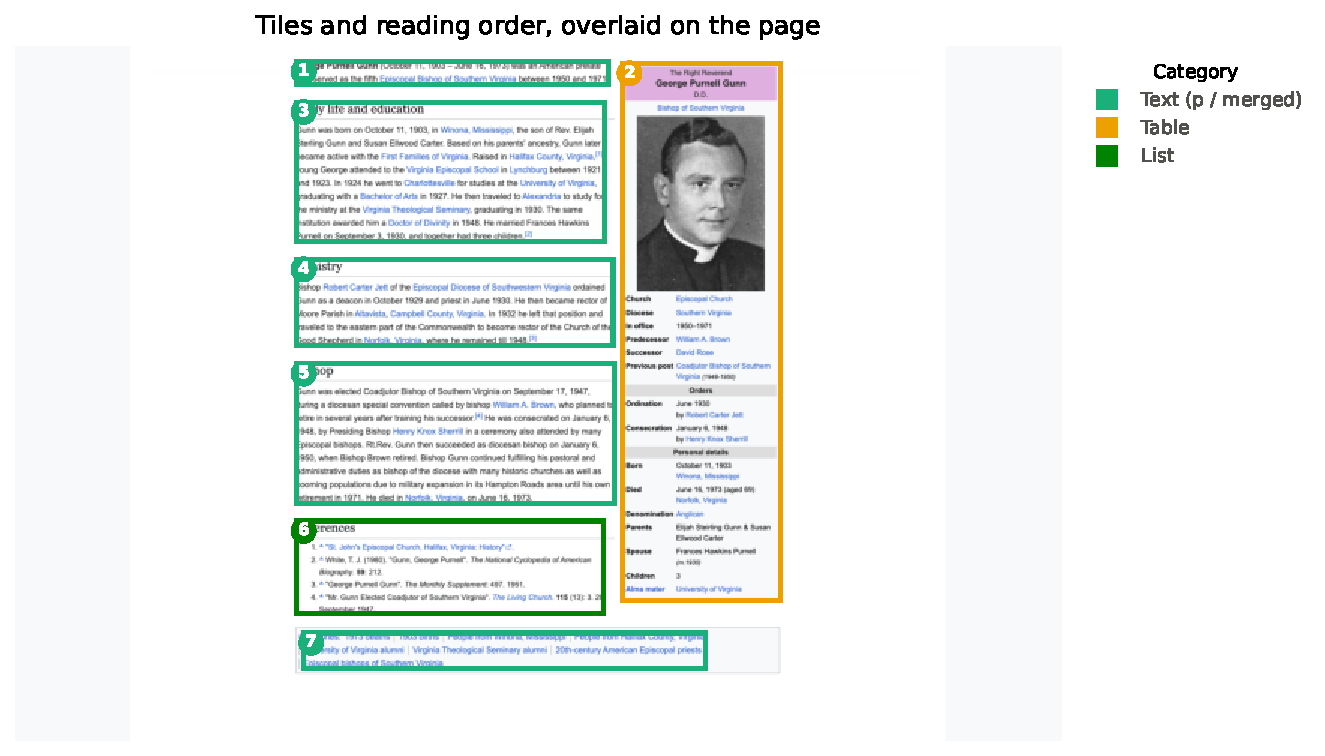
\includegraphics[trim=0 0 0 22pt, clip, width=\linewidth]{tiling_overlay.pdf}
  \caption{Tuilage guidé par le DOM}
  \label{fig-intro_teaser_dom}
\end{subfigure}
\hfill
\begin{subfigure}[b]{0.425\textwidth}
  \centering
  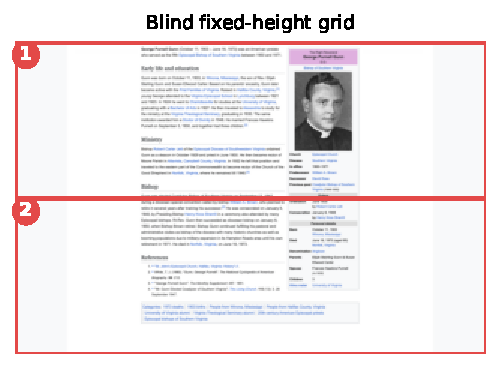
\includegraphics[width=\linewidth]{grid_overlay_illustrative.pdf}
  \caption{Grille de hauteur fixe}
  \label{fig-intro_teaser_grid}
\end{subfigure}
\caption[La même page rendue, tuilée de deux manières]{La même page Wikipédia
rendue (\code{en.wikipedia.org/wiki/George\_P.\_Gunn}), découpée de deux
manières. \textbf{(a)}~Tuilage guidé par le DOM (\cref{sec-tuilage})~:
\textbf{(b)}~Grille aveugle de hauteur fixe selon PixelRAG}
\label{fig-intro_teaser}
\end{figure}

\section*{Contribution personnelle}
\addcontentsline{toc}{section}{Contribution personnelle}

L'intégralité du système décrit dans ce rapport, avec la conception du tuilage,
la construction du graphe, l'entraînement contrastif du lecteur, le contrôleur
budgété, ainsi que le code, les jeux de données synthétiques et les
évaluations qui les accompagnent ont été conçues et implémentées par l'auteur
dans le cadre de ce projet de master. Les deux seuls emprunts à des travaux
tiers, explicitement identifiés comme tels tout au long du rapport, sont
l'architecture de graphe et de contrôleur de MAGE-RAG~\citep{magerag2026},
dont ce travail généralise le contrôleur à des frontières inter-documents
qu'il ne traite pas, et le protocole de grille de PixelRAG~\citep{pixelrag2026},
reproduit à l'identique dans un module indépendant pour servir de condition de
référence à l'\cref{sec-res_ablation_a}. Tout le reste est une contribution
originale de ce projet.

Une version antérieure et condensée des \cref{chap-methodologie,chap-resultats}
a été soumise en double aveugle, sous le titre \emph{\og DOM-Graph RAG:
DOM-Guided Adaptive Tiling and Budgeted Online Evidence Control for
Multimodal Web-Page RAG\fg{}}~\citep{domgraphrag2026}, à l'atelier
\emph{DocInsights 2026}, associé à EMNLP~2026. Le présent rapport en constitue
la version longue~: il ajoute le contexte scientifique complet
(\cref{chap-etat_de_lart}), le détail d'implémentation et d'ingénierie
nécessaire à la reproduction, et l'analyse critique
des quatre évaluations du \cref{chap-resultats}, dont la version courte ne
pouvait rapporter que les résultats les plus saillants.

\section*{Objectifs et contributions}
\addcontentsline{toc}{section}{Objectifs et contributions}

L'objectif de ce projet de master est de transformer l'observation ci-dessus en
un système complet et de mesurer ce qu'elle apporte réellement. Cela suppose de construire quatre composants et de
les évaluer séparément puis ensemble. Les contributions de ce travail sont les
suivantes.

\begin{enumerate}
\item \textbf{Un tuilage adaptatif guidé par le DOM} (\cref{sec-tuilage}) qui
remplace la grille de pixels aveugle de PixelRAG~: chaque élément est recadré
sur sa propre boîte englobante, les éléments trop petits sont fusionnés avec
leurs voisins, ceux trop grands sont subdivisés, et les titres sont
systématiquement appariés avec leur contenu. Le point technique le plus
délicat est la mesure de la boîte englobante des balises de
texte coulant, dont la boîte CSS s'étend sur toute la largeur du conteneur
même lorsque le texte s'enroule autour d'un élément flottant. C'est cette
étape, formalisée en détail au \cref{chap-methodologie}, qui porte
la recherche centrale de ce travail~: aligner la grille de \anglais{patches}
que consomme le modèle vision-langage sur les frontières sémantiques du DOM
plutôt que sur une géométrie arbitraire, de sorte que chaque unité visuelle
soumise à l'encodeur porte un contenu homogène et complet.

\item \textbf{Un graphe de preuves multigranulaire} (\cref{sec-graphe})
organisant les tuiles en deux niveaux (page et élément) et instanciant les cinq
relations du graphe de MAGE-RAG~\citep{magerag2026}, augmentées de deux
relations propres à notre contexte~: \code{links\_to}, qui suit les liens
hypertextes pour relier plusieurs pages, et \code{continues}, qui chaîne les
sections d'une page trop longue pour être traitée d'un bloc.

\item \textbf{Un lecteur vision-langage entraîné par contraste}
(\cref{sec-contrastif}) sur des paires (question, tuile) générées
synthétiquement avec négatifs difficiles minés, adapté par LoRA sur le décodeur
et la tour de vision, via une tête d'encodage de type
PromptEOL~\citep{prompteol2024}.

\item \textbf{Un contrôleur de preuves en ligne budgété} (\cref{sec-controleur})
qui fait évoluer l'état de chaque nœud du graphe selon une politique
best-first sous budget, généralisant l'algorithme de contrôle de MAGE-RAG à des
frontières qui franchissent les limites de document.
\end{enumerate}

À ces contributions logicielles s'ajoute une contribution expérimentale~:
\textbf{quatre évaluations} (\cref{chap-resultats}) qui isolent chaque
composant puis mesurent le système assemblé, avec une attention particulière
portée à la comparabilité des métriques. Nous montrons notamment que le
Recall@$k$ brut n'est pas comparable entre conditions de tuilage, puisqu'un
vivier de candidats plus petit le gonfle mécaniquement, et nous utilisons à la
place un rang percentile invariant à la taille du vivier.

\section*{Résultats principaux}
\addcontentsline{toc}{section}{Résultats principaux}

Deux résultats sont nets. Le tuilage guidé par le DOM double presque la
proportion de questions dont la réponse survit dans une unité récupérable
(\SI{51.8}{\percent} contre \SI{26.4}{\percent} pour la grille de PixelRAG),
tout en consommant \num{2.7} fois moins de pixels par page~; ces deux effets
vont dans le même sens, ce qui est contre-intuitif puisque notre tuilage
produit cinq fois plus de tuiles. L'entraînement contrastif du lecteur fait
presque doubler le Recall@1 sur un partitionnement par article strictement
disjoint ($\num{0.433} \rightarrow \num{0.785}$).

Les composants en aval donnent des résultats plus nuancés, que nous analysons
en détail plutôt que de les minimiser. L'avantage de classement du tuilage DOM
sur la grille est réel mais modeste, et il s'inverse face à un découpage
textuel plat sur le sous-ensemble strictement apparié~: nous montrons que ce
résultat est cohérent avec le scoreur lexical employé, qui n'exploite aucune
information spatiale, et non avec un défaut du tuilage lui-même. Le contrôleur
budgété n'établit pas encore de supériorité sur une sélection top-$k$
statique~; nous en diagnostiquons une cause architecturale identifiable, la
corrigeons, mesurons le gain, et documentons ce qui reste à faire. Enfin,
l'évaluation bout-en-bout montre que le système assemblé échoue par
abstention plutôt que par fabulation, ce qui désigne le sous-rappel de
preuves comme le verrou restant et pointe vers un correctif précis et
déjà instrumenté dans le code.

\section*{Organisation du rapport}
\addcontentsline{toc}{section}{Organisation du rapport}

Le rapport suit une progression en trois chapitres.

Le \textbf{\cref{chap-etat_de_lart}} situe brièvement DOM-Graph RAG dans son
contexte scientifique avec la formulation du problème de récupération et de ses
métriques, le prétraitement des documents visuellement riches, les modèles
vision-langage et la famille du RAG visuel, le RAG structuré par graphe, et
les techniques d'apprentissage contrastif mobilisées ensuite. Il reste volontairement
concis et se clôt sur l'identification précise du
verrou et le positionnement de ce travail face à PixelRAG et MAGE-RAG.

Le \textbf{\cref{chap-methodologie}} constitue le cœur de ce rapport. Il ouvre
sur ce que le navigateur expose réellement de la géométrie d'une page rendue puis
suit l'ordre du pipeline~: rendu et extraction géométrique, tuilage adaptatif
formalisé en détail, construction du graphe, entraînement contrastif du
lecteur et contrôleur en ligne. Chaque étape est explicitée par ses choix de
conception, sa formalisation mathématique, les cas limites rencontrés sur des
pages réelles, et les décisions d'ingénierie qui rendent le pipeline exécutable
sur du matériel modeste.

Le \textbf{\cref{chap-resultats}} présente les quatre évaluations, leur
analyse critique, les coûts de calcul observés, et une discussion structurée des
limites du travail et des directions qu'elles ouvrent.

Un chapitre de conclusion synthétise l'apport et les enseignements du projet,
et les annexes rassemblent les hyperparamètres, l'organisation du dépôt, les
invites utilisées et les protocoles de reproduction.

% =====================================================================
\chapter{État de l'art}
\label{chap-etat_de_lart}
% =====================================================================

Ce chapitre situe DOM-Graph RAG dans son contexte scientifique et se limite à ce qui est strictement nécessaire pour situer les choix de conception~:
le problème du découpage documentaire et ses métriques
(\cref{sec-eda_rag}), le prétraitement des documents visuellement riches
(\cref{sec-eda_docvisuel}), la famille du RAG visuel et son représentant le
plus proche, PixelRAG (\cref{sec-eda_ragvisuel}), le RAG structuré par graphe
et son ancêtre direct, MAGE-RAG (\cref{sec-eda_graphe}), et l'apprentissage
contrastif mobilisé par le lecteur (\cref{sec-eda_contrastif}). Il se clôt sur
le positionnement précis de ce travail (\cref{sec-eda_synthese}).

% =====================================================================
\section{Génération augmentée par récupération et découpage}
\label{sec-eda_rag}
% =====================================================================

La \cref{fig-eda_rag_chaine} donne les trois opérateurs qu'enchaîne un système
RAG. Le découpeur $C : \mathcal{D} \mapsto \mathcal{U}$ transforme une
collection de documents en unités récupérables. Le récupérateur
$R : q \mapsto \mathcal{U}_k \subseteq \mathcal{U}$ sélectionne les $k$ unités
les plus pertinentes pour une question $q$ selon un score $s(q,u)$. Le
générateur $G : (q, \mathcal{U}_k) \mapsto a$ répond à partir de la question
et de ces unités.

\begin{figure}[H]
\centering
\begin{tikzpicture}[
  every node/.style={font=\small},
  op/.style={draw, rounded corners=2pt, minimum width=1.75cm, minimum height=1.0cm,
             align=center, fill=codebg, draw=rulegray, line width=0.7pt},
  focus/.style={op, fill=accent!8, draw=accent, line width=1pt},
  arr/.style={-{Stealth[length=2.0mm]}, thick, draw=black!55},
  lbl/.style={font=\scriptsize, text=black!60, align=center}
]
\node (D) {$\mathcal{D}$};
\node[focus, right=0.5cm of D] (C) {$C$\\[-4pt]{\scriptsize découpeur}};
\node[right=0.5cm of C] (U) {$\mathcal{U}$};
\node[op, right=0.5cm of U] (R) {$R$\\[-4pt]{\scriptsize récupérateur}};
\node[right=0.5cm of R] (Uk) {$\mathcal{U}_k$};
\node[op, right=0.5cm of Uk] (G) {$G$\\[-4pt]{\scriptsize générateur}};
\node[right=0.5cm of G] (a) {$a$};

\draw[arr] (D) -- (C);
\draw[arr] (C) -- (U);
\draw[arr] (U) -- (R);
\draw[arr] (R) -- (Uk);
\draw[arr] (Uk) -- (G);
\draw[arr] (G) -- (a);

\node[lbl, below=1.15cm of Uk] (q) {question $q$};
\draw[arr] (q) -| (R.south);
\draw[arr] (q) -| (G.south);

\node[draw=black!35, dashed, rounded corners=3pt, inner sep=5pt,
      fit=(R)(Uk)(G)] (box) {};
\node[lbl, above=1pt of box.north] {optimisés par la littérature parcourue};
\node[lbl, above=0.30cm of C] {objet de ce travail};
\node[lbl, below=0.28cm of C, text width=2.9cm]
  {fixe le plafond mesuré en \cref{sec-eda_pool}};
\end{tikzpicture}
\caption[Les trois opérateurs d'un système RAG]{Les trois opérateurs d'un
système RAG. La composition impose un ordre de dépendance, car $R$ ne peut
sélectionner que des unités produites par $C$, et $G$ ne peut répondre qu'à
partir de ce que $R$ transmet.}
\label{fig-eda_rag_chaine}
\end{figure}
\citet{rag2020} ont formalisé cette architecture et montré qu'affiner
conjointement l'encodeur de requête et le générateur améliore les tâches à
forte intensité de connaissances~; \citet{fid2021} ont montré qu'encoder
chaque passage séparément avant de les fusionner dans le décodeur permet d'en
traiter un grand nombre sans coût quadratique. \citet{ragsurvey2023} recensent
ces variantes sans qu'aucune ne s'impose.

Le score $s(q,u)$ oppose deux familles. Les approches lexicales
(TF-IDF, BM25~\citep{bm25_2009}) ne demandent aucun entraînement et restent
compétitives~: le \anglais{benchmark} BEIR~\citep{beir2021} établit qu'en
transfert zéro-coup BM25 n'est pas systématiquement dépassé par les
récupérateurs denses, et la \cref{sec-res_ablation_b} retrouve ce constat.
Leur limite est le décalage de vocabulaire. Les approches denses
projettent question et unité dans un espace vectoriel commun appris par
contraste~\citep{sbert2019, simcse2021}~; \citet{dpr2020} en tirent la recette
de référence pour la récupération de passages, et ColBERT~\citep{colbert2020}
en conserve un vecteur par token plutôt qu'un vecteur unique, une idée qui
réapparaît dans le RAG visuel (\cref{sec-eda_ragvisuel}).

Cette littérature suppose $C$ donné, alors qu'il fixe un plafond que ni $R$ ni
$G$ ne peuvent franchir. Si la réponse à $q$ est répartie sur deux unités
distinctes, ou noyée dans une unité majoritairement hors sujet, aucun score ne
peut compenser. Les stratégies de découpage textuel, fenêtres de taille fixe, découpage guidé
par la structure du document ou découpage sémantique aux points de rupture de
similarité entre plongements~\citep{semchunk2025}, sont recensées par
\citet{ragsurvey2023} sans que leur effet sur ce plafond soit mesuré. Toutes
opèrent sur du texte déjà extrait, où les frontières de mise en page ont été
détruites, alors qu'un moteur de rendu les calcule sans coût additionnel sur le
web (\cref{sec-rendu_dom}). Toutes mesurent aussi la qualité du classement en
supposant l'attachement de la réponse acquis, ce que ne fait ni la
\cref{sec-eda_pool} ni la \cref{sec-res_a_attach}.

\subsection{Le biais de taille de vivier}
\label{sec-eda_pool}

Comparer deux stratégies de découpage produisant des viviers de candidats de
tailles différentes pose un piège méthodologique peu discuté~: sur une même
page en \num{5} bandes contre \num{25} tuiles, un classement aléatoire place
la bonne unité au premier rang avec une probabilité de \SI{20}{\percent} dans
le premier cas et de \SI{4}{\percent} dans le second, de sorte que comparer
des Recall@1 bruts revient en partie à comparer des tailles de vivier. Le rang
percentile

\begin{equation}
\mathrm{pct}(u^{+}) = 1 - \frac{\mathrm{rang}(u^{+}) - 1}{n_{\text{items}} - 1},
\label{eq-pctrank}
\end{equation}

vaut $0{,}5$ en espérance sous classement aléatoire quelle que soit la taille
du vivier, et constitue la métrique de comparaison entre conditions de
tuilage employée en \cref{sec-res_ablation_a}, aux côtés du taux
d'attachement qui représente la proportion de questions dont la réponse survit au
découpage, absente des protocoles usuels alors qu'elle détermine le plafond
que ni $R$ ni $G$ ne peuvent franchir.

% =====================================================================
\section{Documents visuellement riches et prétraitement}
\label{sec-eda_docvisuel}
% =====================================================================

Un document est dit visuellement riche lorsque sa mise en page porte de
l'information sémantique, comme un tableau, une facture ou une page à encadrés.
Pour un tel document, la chaîne de prétraitement classique enchaîne trois
étapes à perte, détaillées par la \cref{fig-eda_pertes}. Le résultat cumulé est
qu'une question du type \og quelle est la valeur de la colonne revenus pour la
ligne \num{2024}\fg{} devient difficile à satisfaire, non parce que le
récupérateur est mauvais, mais parce que la correspondance ligne-colonne a été
détruite en amont.

\begin{figure}[H]
\centering
\begin{tikzpicture}[
  every node/.style={font=\small},
  stage/.style={draw, rounded corners=2pt, minimum width=2.55cm, minimum height=0.95cm,
                align=center, fill=codebg, draw=rulegray, line width=0.7pt,
                font=\scriptsize},
  arr/.style={-{Stealth[length=2.0mm]}, thick, draw=black!55},
  etape/.style={font=\scriptsize\itshape, text=black!60, align=center},
  loss/.style={font=\scriptsize, text=black!60, align=center, text width=2.75cm}
]
\node[stage] (doc) {Document\\mis en page};
\node[stage, right=1.6cm of doc] (seq) {Séquence de\\caractères};
\node[stage, right=1.6cm of seq] (ord) {Texte\\réordonné};
\node[stage, right=1.6cm of ord] (unit) {Unités\\récupérables $\mathcal{U}$};

\draw[arr] (doc) -- node[etape, above, text width=1.7cm] {extraction\\ou OCR} (seq);
\draw[arr] (seq) -- node[etape, above, text width=1.7cm] {ordre de\\lecture} (ord);
\draw[arr] (ord) -- node[etape, above, text width=1.7cm] {découpage\\$C$} (unit);

\node[loss, anchor=north] at ($(doc.south)!0.5!(seq.south)+(0,-0.35)$)
  {la structure 2D devient linéaire~; l'OCR y ajoute des erreurs de caractères};
\node[loss, anchor=north] at ($(seq.south)!0.5!(ord.south)+(0,-0.35)$)
  {l'ordre du fichier n'est pas l'ordre de lecture~; heuristiques à taux
   d'erreur non nul};
\node[loss, anchor=north] at ($(ord.south)!0.5!(unit.south)+(0,-0.35)$)
  {frontières d'unité fixées sans égard aux frontières de contenu
   (\cref{sec-eda_rag})};
\end{tikzpicture}
\caption[Les trois pertes de la chaîne de prétraitement classique]{Les trois
étapes à perte de la chaîne de prétraitement classique et l'information détruite
à chacune. Les modèles sensibles à la mise en page réinjectent la géométrie en
aval de la première étape~; les modèles sans OCR suppriment les deux premières.}
\label{fig-eda_pertes}
\end{figure}

Une première réponse injecte la géométrie dans la représentation.
LayoutLM~\citep{layoutlm2020} ajoute aux plongements de tokens des positions 2D
dérivées de la boîte englobante de chaque mot~; LayoutLMv2~\citep{layoutlmv2_2021}
et LayoutLMv3~\citep{layoutlmv3_2022} l'intègrent au pré-entraînement (\num{92.1}
de $F_1$ sur FUNSD, \num{83.4} d'ANLS sur DocVQA~\citep{docvqa2021})~; MarkupLM~\citep{markuplm2022}
transpose l'idée au web en encodant le chemin XPath de chaque token. Ces
modèles reçoivent tous des mots et boîtes déjà produits par un OCR en amont, et
la structure y est apprise, donc coûteuse à ré-entraîner sur un type de
document non couvert~; surtout, elle sert la représentation d'une unité déjà
découpée, non la décision de découpage~: MarkupLM sait que deux tokens
partagent un ancêtre DOM, il ne décide pas où couper la page.

Une seconde réponse supprime l'OCR~: Donut~\citep{donut2022} produit du texte
structuré directement depuis l'image d'un document, et
Pix2Struct~\citep{pix2struct2023} porte l'idée au web en pré-entraînant sur
\num{80} millions de captures d'écran, avec pour cible un HTML simplifié dérivé
du DOM rendu. Cela permet ainsi d'établir que le DOM porte la structure dont un
modèle visuel a besoin, mais il l'exploite comme cible de supervision apprise,
quand ce travail l'emploie comme décision de découpage à l'inférence, sans
apprentissage.

% =====================================================================
\section{Modèles vision-langage et RAG visuel}
\label{sec-eda_ragvisuel}
% =====================================================================

Les modèles vision-langage contemporains combinent une tour de vision de type
\anglais{Vision Transformer}~\citep{vit2021}, qui découpe l'image en
\anglais{patches} traités par auto-attention~\citep{transformer2017}, et un
modèle de langue décodeur consommant une séquence mixte de tokens visuels et
textuels, sur la base des représentations image-texte alignées par
contraste~\citep{clip2021}. Qwen2-VL~\citep{qwen2vl2024}, employé au
\cref{chap-methodologie}, apporte le support de la résolution dynamique~: le
nombre de tokens visuels y est proportionnel à l'aire réelle de l'image, une
propriété dont le \cref{sec-eda_cout_visuel} tire les conséquences pour ce
travail.

Si un tel modèle produit un plongement d'image aligné sur le langage, on peut
indexer des images de pages entières et récupérer dessus~: \anglais{Document
Screenshot Embedding}~\citep{dse2024} le fait sans extraction de contenu
préalable, et ColPali~\citep{colpali2024} porte le mécanisme d'interaction
tardive de ColBERT aux \anglais{patches} visuels.

\subsection{PixelRAG et le découpage aveugle}
\label{sec-eda_pixelrag}

Le travail le plus directement relié est PixelRAG~\citep{pixelrag2026}, qui
applique cette approche à l'échelle du web~: les pages sont rendues, découpées
en bandes et indexées avec un encodeur vision-langage, et les auteurs
rapportent égaler ou dépasser la récupération textuelle sur plusieurs bancs
d'essai, avec une réduction du coût en tokens allant jusqu'à un facteur trois
par sous-échantillonnage de la résolution. C'est son découpage qui nous
intéresse~: une grille de hauteur fixe, la page rendue tranchée en bandes de
$\num{875} \times \num{1024}$ pixels indépendamment de leur contenu. La
décision est simple et sans dépendance au type de document, mais son défaut
est celui de la fenêtre de taille fixe qui crée une bande coupant là où elle tombe,
au milieu d'un tableau comme d'un paragraphe. C'est cette condition qui est
réimplémentée (\cref{sec-protocole_grille}) et mesurée
(\cref{sec-res_ablation_a}).

% =====================================================================
\section{RAG structuré par graphe}
\label{sec-eda_graphe}
% =====================================================================

Traiter $\mathcal{U}$ comme un sac plat empêche de récupérer une unité peu
pertinente lexicalement mais indispensable contextuellement, et interdit le
raisonnement multi-sauts. Deux issues coexistent~: itérer la récupération ou
structurer les preuves en amont. La première voie est celle de
ReAct~\citep{react2023}, IRCoT~\citep{ircot2023}, FLARE~\citep{flare2023} et
Self-RAG~\citep{selfrag2024}, qui entrelacent raisonnement et appels de
récupération, au prix d'appels au modèle en série. Dans la seconde,
\citet{graphrag2024} construisent un graphe de connaissances
sur des entités extraites par un modèle de langue, ce qui répond à des
questions globales sur un corpus qu'aucune récupération locale ne
satisferait~; le graphe porte sur des entités, non sur la structure
documentaire.

\subsection{MAGE-RAG}
\label{sec-eda_magerag}

\citet{magerag2026} construisent au contraire un graphe de la structure
du document, et c'est l'ancêtre direct de l'architecture proposée ici~: des
nœuds de niveau page et de niveau élément, reliés par cinq relations
(\code{contains}, \code{reading\_order}, \code{layout\_adjacency},
\code{section\_hierarchy}, \code{semantic\_neighbor}), que parcourt à la
requête un contrôleur budgété décidant quels nœuds le modèle lecteur ouvre
réellement. L'\cref{sec-controleur} en généralise l'algorithme. La
différence tient à la provenance du graphe~: MAGE-RAG le construit hors ligne,
à partir d'un document déjà segmenté et d'un ordre de lecture déjà
déterminé, quand celui construit ici l'est depuis le DOM d'une page rendue, qui
fournit sans coût additionnel frontières exactes et types d'éléments
(\cref{sec-rendu_dom}). Deux relations que le contexte web rend
nécessaires s'y ajoutent, \code{links\_to} et \code{continues}
(\cref{tab-graphe_relations}). MAGE-RAG est évalué sur LongDocURL et
MMLongBench-Doc, deux jeux de données constitués de PDF déjà analysés~; ces
chiffres sont rapportés au \cref{chap-resultats} comme référence de
l'architecture, non comme comparaison numérique, faute d'un DOM à exploiter
sur un PDF.

% =====================================================================
\section{Apprentissage contrastif et adaptation efficace}
\label{sec-eda_contrastif}
% =====================================================================

\subsection{InfoNCE et la qualité des négatifs}
\label{sec-eda_contrastif_infonce}

Entraîner un récupérateur revient à apprendre une similarité $s(q,u)$ qui
place la bonne unité plus près de la question que les mauvaises. L'objectif
standard, InfoNCE~\citep{cpc2018}, largement repris en vision~\citep{simclr2020},
s'écrit pour une question de plongement $\mathbf{z}_q$, une unité positive
$u^+$ et des négatifs $\{u_1^-,\dots,u_K^-\}$~:

\begin{equation}
\mathcal{L}_{\text{InfoNCE}}
= -\log
\frac{\exp\!\big(\mathrm{sim}(\mathbf{z}_q, \mathbf{z}_{u^{+}}) / \tau\big)}
     {\exp\!\big(\mathrm{sim}(\mathbf{z}_q, \mathbf{z}_{u^{+}}) / \tau\big)
      + \sum_{i=1}^{K}
      \exp\!\big(\mathrm{sim}(\mathbf{z}_q, \mathbf{z}_{u^{-}_i}) / \tau\big)},
\label{eq-infonce}
\end{equation}

où $\tau$ est une température qui concentre le gradient sur les négatifs
proches du positif à mesure qu'elle diminue. Tout dépend des négatifs~: les
\anglais{in-batch negatives}~\citep{dpr2020} réutilisent gratuitement les
positifs des autres exemples du lot, tandis que les négatifs difficiles sont
minés délibérément. Le \cref{sec-contrastif} reprend cette équation, l'étend
au lot entier, et l'analyse plus en détail. La génération synthétique de
paires question-passage, établie par InPars~\citep{inpars2022} et
Promptagator~\citep{promptagator2022}, est transposée ici à des tuiles
d'image.

\subsection{Adaptation efficace d'un modèle génératif en encodeur}
\label{sec-eda_contrastif_adaptation}

Affiner intégralement un modèle de plusieurs milliards de paramètres est hors
de portée d'une infrastructure académique modeste. LoRA~\citep{lora2021} gèle
les poids pré-entraînés et n'apprend, pour chaque matrice ciblée, qu'une mise à
jour de rang faible~; QLoRA~\citep{qlora2023} y ajoute la quantification du
modèle gelé. Dans le cas multimodal, LoRA peut cibler le décodeur seul ou
aussi la tour de vision puisque la tâche traitée au \cref{sec-contrastif_lora}
exige les deux. Un second obstacle est que ces modèles sont génératifs et
n'exposent aucun vecteur de représentation~; PromptEOL~\citep{prompteol2024}
fait suivre l'entrée d'une amorce à compléter et prend l'état caché du
dernier token comme plongement, un procédé appliqué à l'identique à une
question textuelle et à une image de tuile au \cref{sec-contrastif_encodeur}.

% =====================================================================
\section{Synthèse et positionnement}
\label{sec-eda_synthese}
% =====================================================================

Trois constats délimitent une lacune précise, que le
\cref{tab-eda_positionnement} résume.

\begin{table}[H]
\centering
\small
\caption[Positionnement de DOM-Graph RAG]{Origine des frontières de l'unité
récupérable chez les travaux les plus proches. Elles sont soit arbitraires,
fenêtre ou grille, soit héritées d'un découpage effectué ailleurs, format du
fichier source ou corpus déjà segmenté en amont.}
\label{tab-eda_positionnement}
\begin{tabular}{@{}ll@{}}
\toprule
\textbf{Travail} & \textbf{Origine des frontières} \\
\midrule
\multicolumn{2}{@{}l}{\emph{Récupération textuelle}} \\
\quad DPR~\citep{dpr2020} & fenêtre fixe \\
\quad GraphRAG~\citep{graphrag2024} & fenêtre fixe \\[3pt]
\multicolumn{2}{@{}l}{\emph{Modèles sensibles à la mise en page}} \\
\quad LayoutLM~\citep{layoutlm2020} & corpus segmenté en amont \\
\quad MarkupLM~\citep{markuplm2022} & corpus segmenté en amont \\[3pt]
\multicolumn{2}{@{}l}{\emph{RAG visuel, lecture des pixels}} \\
\quad DSE~\citep{dse2024} & format du fichier source, la page \\
\quad ColPali~\citep{colpali2024} & format du fichier source, la page \\
\quad PixelRAG~\citep{pixelrag2026} & grille de hauteur fixe \\[3pt]
\multicolumn{2}{@{}l}{\emph{RAG par graphe de structure}} \\
\quad MAGE-RAG~\citep{magerag2026} & corpus segmenté en amont \\
\midrule
\textbf{Ce travail}, pixels et graphe & \textbf{boîtes englobantes du DOM rendu} \\
\bottomrule
\end{tabular}
\end{table}
Premièrement, le RAG visuel démontre que lire les pixels préserve une
information que l'extraction textuelle détruit, mais ne traite pas le
découpage~: soit il l'évite en travaillant à l'échelle de la page, soit il le tranche à
l'aveugle, comme PixelRAG. Deuxièmement, les modèles sensibles à la
mise en page exploitent la structure, mais en l'apprenant à grands frais et
pour représenter des unités déjà découpées. Enfin, MAGE-RAG
démontre qu'un contrôleur de graphe budgété surpasse une sélection top-$k$
statique, mais suppose les éléments du document déjà constitués en amont de
son propre pipeline, c'est-à-dire l'artefact que PixelRAG jette au rendu et que
ce travail restitue.

La thèse défendue est que, pour une page web sémantiquement balisée, la
segmentation dont le RAG visuel a besoin est déjà disponible et exacte dans le
DOM de la page rendue, et qu'il est donc inutile de la reconstruire depuis les
pixels ou de la contourner par une grille. Le \cref{chap-methodologie} formalise
et met à l'épreuve cette thèse, en commençant précisément là où PixelRAG
s'arrête~: par ce qu'un navigateur expose de la géométrie d'une page rendue.
% =====================================================================
\chapter{Méthodologie}
\label{chap-methodologie}
% =====================================================================

Ce chapitre décrit le système construit pour mettre à l'épreuve la thèse formulée
au chapitre précédent, et en détaille la formalisation mathématique. Il commence
par établir ce qu'un navigateur expose réellement de la géométrie d'une page
rendue (\cref{sec-rendu_dom}) représentant le préalable technique dont dépendent tous les
choix qui suivent, puis suit l'ordre de la chaîne de traitement~: une page est
rendue une fois par un navigateur sans interface graphique et sa géométrie est
mesurée (\cref{sec-rendu})~; cette géométrie pilote un tuilage adaptatif, dont
la \cref{sec-tuilage} formalise les règles et le modèle de coût
(\cref{sec-tuilage})~; les tuiles sont organisées en un graphe à deux niveaux,
éventuellement étendu à plusieurs pages liées (\cref{sec-graphe})~; un lecteur
vision-langage est entraîné par contraste, hors ligne, à évaluer la pertinence
d'une paire (question, tuile) (\cref{sec-contrastif})~; enfin, à la requête, un
contrôleur en ligne parcourt le graphe sous budget pour décider quels nœuds le
lecteur ouvre réellement (\cref{sec-controleur}). La \cref{sec-implementation}
détaille les choix d'ingénierie qui rendent l'ensemble exécutable, et la
\cref{sec-protocole} la construction des jeux de données évalués au
\cref{chap-resultats}.

\begin{figure}[H]
\centering
\begin{tikzpicture}[
  node distance=0.62cm,
  every node/.style={font=\small},
  stage/.style={draw, rounded corners=2pt, minimum width=7.2cm, minimum height=0.86cm,
                align=center, fill=codebg, draw=rulegray, line width=0.7pt},
  online/.style={stage, fill=accent!6, draw=accent, line width=0.9pt},
  offline/.style={stage},
  arr/.style={-{Stealth[length=2.2mm]}, thick, draw=black!55},
  tag/.style={font=\scriptsize\itshape, text=black!55, align=left}
]
\node[offline] (render) {Rendu de page et extraction géométrique\\[-2pt]
  {\scriptsize Playwright, retrait du bruit d'interface, boîtes englobantes}};
\node[offline, below=of render] (tiling) {Tuilage adaptatif et découpe\\[-2pt]
  {\scriptsize appariement des titres, fusion, chevauchements}};
\node[offline, below=of tiling] (graph) {Graphe multigranulaire\\[-2pt]
  {\scriptsize 1 nœud page $+$ $N$ nœuds élément, 7 relations, corpus multi-pages}};
\node[offline, below=of graph] (train) {Lecteur entraîné par contraste\\[-2pt]
  {\scriptsize QA synthétique, négatifs difficiles, LoRA sur ViT $+$ décodeur}};
\node[online, below=of train] (ctrl) {Contrôleur de preuves budgété\\[-2pt]
  {\scriptsize \anglais{best-first} sous budget, machine à quatre états}};
\node[online, below=of ctrl] (answer) {Synthèse de la réponse\\[-2pt]
  {\scriptsize lecture des tuiles ouvertes, puis génération}};

\draw[arr] (render) -- (tiling);
\draw[arr] (tiling) -- (graph);
\draw[arr] (graph) -- (train);
\draw[arr] (train) -- (ctrl);
\draw[arr] (ctrl) -- (answer);

\node[tag, right=0.3cm of render.east, anchor=west] {\cref{sec-rendu}};
\node[tag, right=0.3cm of tiling.east, anchor=west] {\cref{sec-tuilage}};
\node[tag, right=0.3cm of graph.east, anchor=west] {\cref{sec-graphe}};
\node[tag, right=0.3cm of train.east, anchor=west] {\cref{sec-contrastif}};
\node[tag, right=0.3cm of ctrl.east, anchor=west] {\cref{sec-controleur}};

\node[rotate=90, anchor=south, font=\scriptsize\bfseries, text=black!55]
  at ([xshift=-0.55cm]$(render.west)!0.5!(train.west)$)
  {hors ligne, une fois par page};
\node[rotate=90, anchor=south, font=\scriptsize\bfseries, text=accent]
  at ([xshift=-0.55cm]$(ctrl.west)!0.5!(answer.west)$)
  {en ligne, par requête};
\end{tikzpicture}
\caption[Vue d'ensemble de la chaîne de traitement]{Vue d'ensemble de la chaîne
DOM-Graph RAG}
\label{fig-pipeline}
\end{figure}

% =====================================================================
\section{Préliminaires géométriques : le DOM et le moteur de rendu}
\label{sec-rendu_dom}
% =====================================================================

L'hypothèse centrale de ce travail est que la segmentation nécessaire au RAG
visuel est déjà présente dans le DOM d'une page rendue. Cette section établit
quelle information le navigateur expose, où se situent les pièges, et pose la
notation reprise par le reste du chapitre.

\subsection{Du balisage à la mise en page, et le modèle de boîtes}
\label{sec-rendu_boites}

Le traitement d'une page par un navigateur enchaîne quatre étapes. L'analyse du
HTML produit le DOM, un arbre $T = (V, E)$ dont chaque nœud $v \in V$
correspond à un élément ou à un nœud texte. La cascade attribue ensuite à chaque
élément ses valeurs de propriétés calculées. La mise en forme (\anglais{reflow})
détermine la position et les dimensions exactes de chaque boîte dans un repère
absolu. La peinture produit enfin les pixels.

La mise en forme se termine intégralement avant que le premier pixel ne soit
peint, si bien que la géométrie de tout élément est déjà connue au moment de la
peinture. Un système qui recadre des régions
dans l'image peinte travaille donc en aval d'une source de vérité géométrique
qu'il n'a jamais consultée.

La fonction $\mathcal{B} : V \to \mathbb{R}_{\geq 0}^4$ associe à un élément
rendu sa boîte $\mathcal{B}(v) = (x_v, y_v, w_v, h_v)$ dans le repère absolu du
document, où $(x_v, y_v)$ est le coin supérieur gauche et $(w_v, h_v)$ la
largeur et la hauteur. C'est elle qu'exploite le tuilage de la
\cref{sec-tuilage}, aucune partie de la chaîne ne redérivant une géométrie que
le navigateur a déjà calculée.

Une boîte est faite de quatre régions concentriques, contenu,
\anglais{padding}, bordure et marge. Les API de géométrie rapportent par défaut
celle qui correspond visuellement à l'élément, et $\mathcal{B}$ désigne
implicitement cette région.

Le type d'affichage détermine le comportement de $\mathcal{B}$. Un élément de
type \textbf{bloc} (\code{<p>}, \code{<div>}, \code{<h1>}--\code{<h6>},
\code{<ul>}) a par défaut \code{width: auto}, donc $w_v = w_{\op{parent}(v)}$
quel que soit son contenu. Un titre de trois mots dans une colonne de
\SI{1200}{\pixel} a ainsi une boîte de \SI{1200}{\pixel} de large. Un élément de
type \textbf{en ligne} (\code{<span>}, \code{<a>}, \code{<em>}) ne forme pas une
boîte unique mais autant de rectangles que de fragments de ligne. Un
\code{<table>}, enfin, s'ajuste à son contenu au lieu de remplir son conteneur.
La difficulté décrite ci-dessous ne frappe donc que les blocs de texte.

\subsection{Éléments flottants : l'écart entre boîte de bloc et lignes réelles}
\label{sec-eda_dom_float}

Le cas déterminant pour la mesure des tuiles est celui des éléments flottants.
Un élément déclaré \code{float: right} est retiré du flux normal et poussé sur
le bord droit de son conteneur, et le contenu en ligne des blocs qui le suivent
s'enroule autour de lui. L'effet est asymétrique. Pour un bloc $v$ qui suit un
flottant, $\mathcal{B}(v)$ n'est pas réduite et continue de s'étendre sur
$w_{\op{parent}(v)}$ en passant sous le flottant, alors que seules les lignes de
texte à l'intérieur de $v$ sont raccourcies. La \cref{fig-eda_float} met les
deux géométries en regard.

\begin{figure}[H]
\centering
\begin{subfigure}[b]{0.50\textwidth}
\centering
\begin{tikzpicture}[scale=0.88, every node/.style={font=\scriptsize}]
\draw[draw=rulegray, line width=0.8pt, fill=codebg] (0,0) rectangle (7.0,4.9);
\node[anchor=north west, text=black!55] at (0.08,4.84) {conteneur};
\draw[draw=black!45, fill=black!12, line width=0.7pt] (4.75,2.30) rectangle (6.85,4.50);
\node[align=center, text=black!60] at (5.80,3.40) {élément\\flottant};
\draw[draw=accent, dashed, line width=1.0pt] (0.18,0.52) rectangle (6.85,4.16);
\foreach \y in {3.94,3.60,3.26,2.92,2.58}{
  \draw[draw=codestr, line width=0.8pt, fill=codestr!12] (0.32,\y-0.12) rectangle (4.55,\y+0.12);
}
\foreach \y in {2.10,1.76,1.42,1.08}{
  \draw[draw=codestr, line width=0.8pt, fill=codestr!12] (0.32,\y-0.12) rectangle (6.68,\y+0.12);
}
\draw[draw=codestr, line width=0.8pt, fill=codestr!12] (0.32,0.62) rectangle (2.60,0.86);
\draw[draw=accent, dashed, line width=1.0pt] (0.20,-0.65) -- (0.95,-0.65);
\node[anchor=west, text=black!65] at (1.05,-0.65) {\code{getBoundingClientRect}};
\draw[draw=codestr, line width=0.8pt, fill=codestr!12] (0.20,-1.32) rectangle (0.95,-1.10);
\node[anchor=west, text=black!65] at (1.05,-1.21) {\code{getClientRects}, nœuds texte};
\end{tikzpicture}
\caption{Les deux géométries d'un même bloc}
\label{fig-eda_float_schema}
\end{subfigure}
\hfill
\begin{subfigure}[b]{0.455\textwidth}
\centering
\begin{tikzpicture}
\node[anchor=south west, inner sep=0] (img)
  {\includegraphics[height=6.0cm, trim=179 38 180 2, clip]{extracted-000.png}};
\begin{scope}[x={(img.south east)}, y={(img.north west)}]
  \draw[draw=accent, dashed, line width=0.9pt] (0.024,0.102) rectangle (0.982,0.239);
  \draw[draw=codestr, line width=0.9pt] (0.038,0.105) rectangle (0.655,0.236);
\end{scope}
\end{tikzpicture}
\caption{La liste de références d'une page réelle}
\label{fig-eda_float_reel}
\end{subfigure}
\caption[Boîte de bloc et rectangles de lignes]{\textbf{(a)}~Un élément flottant à droite raccourcit les
lignes des blocs qui le suivent sans réduire leur boîte de bloc, laquelle
continue de passer sous lui. \textbf{(b)}~La boîte de bloc de la liste de références, en tirets,
s'étend sous l'infoboîte, alors que l'union de ses rectangles de lignes s'arrête à son bord}
\label{fig-eda_float}
\end{figure}

La correction employée en \cref{sec-rendu_textflow} se formalise ainsi. Soit $v$
un élément de texte coulant et $N_1, \dots, N_k$ ses nœuds texte descendants.
\code{getClientRects}, appliqué à un objet \code{Range} construit sur chaque
$N_i$, retourne les rectangles de ligne effectivement rendus
$\{r_{i,1}, \dots, r_{i,m_i}\}$. Chaque $r$ est un quadruplet
$(x^{(0)}, y^{(0)}, x^{(1)}, y^{(1)})$ de coordonnées de coins. La boîte serrée
est l'enveloppe rectangulaire de leur union.
\begin{equation}
\mathcal{B}_{\text{serré}}(v) = \Big[
  \min_{i,j} x^{(0)}_{i,j},\;
  \min_{i,j} y^{(0)}_{i,j},\;
  \max_{i,j} x^{(1)}_{i,j} - \min_{i,j} x^{(0)}_{i,j},\;
  \max_{i,j} y^{(1)}_{i,j} - \min_{i,j} y^{(0)}_{i,j}
\Big].
\label{eq-boite_serree}
\end{equation}
Le \code{Range} doit être construit sur les nœuds texte et non sur
l'élément lui-même. Un \code{Range} englobant tout $v$ retournerait en plus le
rectangle de sa boîte pleine largeur, ce qui ramènerait l'union à
$\mathcal{B}(v)$. Un nœud texte n'a par construction aucune boîte propre, et ses
rectangles ne peuvent donc être que des lignes réellement rendues.

En l'absence de flottant, $\mathcal{B}_{\text{serré}}(v) = \mathcal{B}(v)$, les
lignes remplissant la largeur du bloc. En présence d'un flottant qui intersecte
les rangées de $v$, la boîte serrée est strictement plus étroite, et l'écart
d'aire
\begin{equation}
\Delta A(v) = \op{aire}\big(\mathcal{B}(v)\big) - \op{aire}\big(\mathcal{B}_{\text{serré}}(v)\big) \;\geq\; 0
\label{eq-aire_perdue}
\end{equation}
mesure le fond blanc qu'un recadrage sur $\mathcal{B}(v)$ soumettrait en pure
perte à l'encodeur visuel. C'est ce terme, sommé sur toutes les balises de texte
coulant d'une page, que la mesure serrée de la \cref{sec-rendu_textflow}
élimine, et dont la \cref{sec-res_a_pixels} rapporte l'effet agrégé sur le
pixels par page.

Pour un \code{<table>}, un \code{<figure>} ou un \code{<img>}, en revanche,
bordure, fond et marge intérieure font partie du contenu visuel. La boîte brute
$\mathcal{B}(v)$ y reste la mesure correcte, et $\Delta A(v) = 0$ par
convention.

\subsection{Les deux API de géométrie et le repère absolu}
\label{sec-eda_dom_api}

Le navigateur expose deux méthodes de mesure. \code{getBoundingClientRect}
retourne $\mathcal{B}(v)$, et \code{getClientRects} la liste des rectangles
effectivement occupés, base de $\mathcal{B}_{\text{serré}}$ ci-dessus. Toutes
deux sont relatives au \anglais{viewport} et non au document, alors que le
recadrage d'une capture pleine page exige le repère absolu. Le décalage de
défilement courant $(s_x, s_y)$ leur est donc ajouté.
\begin{equation}
\mathcal{B}_{\text{abs}}(v) = \mathcal{B}_{\text{viewport}}(v) + (s_x, s_y, 0, 0).
\label{eq-repere_absolu}
\end{equation}
Cette conversion est appliquée systématiquement à l'extraction
(\cref{sec-rendu}). La profondeur d'un nœud dans $T$ fournit par ailleurs un
ordre de traitement commode pour résoudre l'imbrication
(\cref{sec-tuilage_elagage}), un parent étant toujours à une profondeur
strictement inférieure à celle de ses descendants.

\subsection{Ordre du DOM et ordre visuel}
\label{sec-eda_dom_ordre}

L'ordre des nœuds dans $T$ est celui dans lequel l'auteur a écrit le balisage,
et non l'ordre de lecture visuel, le positionnement CSS pouvant faire diverger
les deux arbitrairement. Le déduire du parcours de $T$ produirait, sur une mise
en page non triviale, une séquence qui ne correspond pas à ce qu'un lecteur
humain suit. La relation d'ordre de lecture
(\cref{sec-graphe_ordre}) est donc calculée par une heuristique spatiale sur les
coordonnées $\mathcal{B}_{\text{abs}}$ plutôt que par un parcours de $T$. Le DOM
fournit $\mathcal{B}$ et les types d'éléments, pas un ordre de lecture total.

% =====================================================================
\section{Rendu de page et extraction géométrique}
\label{sec-rendu}
% =====================================================================

\subsection{Rendu sans interface graphique}

La page est chargée sans interface graphique, via Playwright, avec une largeur
de fenêtre d'affichage de \SI{2048}{\pixel} et un facteur d'échelle de
périphérique de \num{1}. La hauteur de la fenêtre, fixée à \SI{1000}{\pixel},
est sans effet, la capture pleine page produisant une image de la hauteur totale
du document rendu, soit plusieurs dizaines de milliers de pixels sur les
articles les plus longs (\cref{sec-tuilage_sections}).

La largeur de \SI{2048}{\pixel} égale la hauteur maximale de tuile
(\cref{sec-tuilage_regles}), de sorte que la plus grande unité produite est un
carré de \num{2048} pixels de côté et qu'un seul paramètre borne l'aire maximale
soumise à l'encodeur. Elle n'améliore en revanche pas la résolution du texte, la
taille en pixels d'un caractère ne dépendant pas de la largeur de fenêtre à
facteur d'échelle constant. Élargir le rendu ajoute de la marge, non de la
définition.

Cette marge n'est pas neutre pour le \cref{chap-resultats}. La colonne de
contenu occupe environ \SI{40}{\percent} de la largeur de rendu
(\cref{fig-tuiles_reelles}), si bien qu'une bande de grille est majoritairement
du fond blanc là où une tuile mesurée serrée (\cref{sec-rendu_textflow}) ne
l'est pas. Le rapport de budget de pixels de la \cref{sec-res_a_pixels} est
mesuré à cette largeur et décroît avec elle.

\paragraph{Ordre des opérations.} Le chargement attend la condition
\code{networkidle}, et l'extraction géométrique est évaluée après la capture
pleine page, la condition d'attente étant réévaluée entre les deux. La capture
fait en effet défiler le document et déclenche le chargement différé des images,
qui modifie la hauteur des blocs qui les contiennent. Une mesure prise avant ce
défilement décrirait une mise en page antérieure au chargement, et les
recadrages seraient décalés d'autant sans qu'aucune métrique ne le signale.

\subsection{Retrait du bruit d'interface}

Avant la capture, un ensemble de sélecteurs CSS retire du document le bruit
d'interface, c'est-à-dire les barres de navigation, pieds de page, panneaux
latéraux du logiciel de wiki, bandeaux d'avertissement, liens d'édition de
section et boîtes de navigation. Ces éléments ne portent aucune information sur
le sujet de la page et produiraient des tuiles coûteuses en pixels et
systématiquement non pertinentes.

{\sloppy
La liste combine des sélecteurs génériques (\code{nav}, \code{footer},
\code{header}, \code{script}, \code{style}) et des sélecteurs propres à MediaWiki
(\code{\#mw-navigation}, \code{.vector-header}, \code{.navbox},
\code{.mw-editsection}, \code{.noprint}). Cette seconde catégorie est une
dépendance explicite au type de site et constitue la principale limite de portée
des résultats quantitatifs (\cref{sec-res_limites}). Elle porte sur le nettoyage
et non sur la logique de tuilage.
\par}

\subsection{Extraction des boîtes englobantes}

L'extraction est un unique appel de fonction JavaScript évalué dans le contexte
de la page. Pour un ensemble configurable de balises (\code{h1} à \code{h4},
\code{p}, \code{table}, \code{figure}, \code{img}, \code{ul}, \code{ol},
\code{blockquote}, \code{pre}), le script relève, pour chaque élément
correspondant, sa position absolue au sens de l'\cref{eq-repere_absolu}, ses
dimensions, un aperçu de son texte, sa profondeur dans l'arbre DOM et, le cas
échéant, les liens hypertextes qu'il contient.

\paragraph{Extraction sélective des liens.} Les liens ne sont relevés que pour
les éléments \code{p}. Une page encyclopédique porte quelques dizaines de liens
dans son texte et plusieurs centaines dans ses tableaux, boîtes de navigation et
listes de références, dont le suivi ferait croître le coût du parcours de corpus
(\cref{sec-graphe_corpus}) sans apporter de contenu pertinent. Les liens
conservés sont résolus en URL absolue via \code{document.baseURI}, les ancres
internes et les schémas non HTTP étant écartés.

\subsection{Mesure serrée des balises de texte coulant}
\label{sec-rendu_textflow}

Recadrer sur $\mathcal{B}$ plutôt que sur $\mathcal{B}_{\text{serré}}$ produit
deux défauts mesurables, l'un et l'autre conséquences de l'asymétrie formalisée
en \cref{sec-eda_dom_float}.

Le premier est un double comptage. Recadrer sur $\mathcal{B}(v)$ capture les
pixels de l'élément flottant voisin en plus du contenu visé, et ces pixels
apparaissent alors dans deux unités de récupération, celle du bloc et celle de
l'infoboîte. Le budget est payé deux fois, et les scores de pertinence de deux
tuiles sont alimentés par le même contenu.

Le second est un coût. Une tuile de texte recadrée sur $\mathcal{B}(v)$ consomme
la même surface qu'une bande de grille quel que soit son contenu réel, soit
\num{2058000} pixels en moyenne contre \num{157170} pour une tuile recadrée sur
$\mathcal{B}_{\text{serré}}(v)$ (\cref{sec-res_a_pixels}). Le cas dominant est
la liste de références en fin d'article, rendue en \code{<ol>}, dont la boîte
traverse toute la largeur du conteneur alors que ses lignes occupent une colonne
étroite (\cref{fig-eda_float_reel}).

Le tuilage recadre donc sur $\mathcal{B}_{\text{serré}}(v)$ pour les balises
dont la boîte de bloc est structurellement plus large que leur contenu
(\code{h1} à \code{h4}, \code{p}, \code{blockquote}, \code{ul}, \code{ol}),
désignées balises de texte coulant et configurables. Un \code{TreeWalker}
parcourt les nœuds texte non vides de $v$, un \code{Range} est construit sur le
contenu de chacun, et l'\cref{eq-boite_serree} est évaluée sur l'union des
rectangles retournés par \code{getClientRects}. La granularité du \code{Range}
est imposée par la contrainte établie en \cref{sec-eda_dom_float}. Les autres
balises conservent $\mathcal{B}(v)$, avec $\Delta A(v) = 0$.

% =====================================================================
\section{Tuilage adaptatif guidé par le DOM}
\label{sec-tuilage}
% =====================================================================

Le tuilage instancie pour le cas web le découpeur
$C : \mathcal{D} \mapsto \mathcal{U}$ de la \cref{sec-eda_rag}. La fonction
$C_{\text{DOM}}$ définie ci-dessous, construite à partir de $\mathcal{B}$ et
$\mathcal{B}_{\text{serré}}$ (\cref{sec-rendu_dom}), remplace la grille de
hauteur fixe de PixelRAG. Elle transforme une liste d'éléments géolocalisés $E$
et une capture pleine page $I$ en une liste de tuiles
$T = C_{\text{DOM}}(E, I)$, chacune formée d'un recadrage d'image accompagné de
ses coordonnées, de la balise DOM d'origine, d'un aperçu textuel, des
identifiants des éléments sources et des liens agrégés.

Le nombre de tuiles retenues par unité de page est borné à \num{25}. Cette
borne est héritée du coût de génération des paires question-réponse
(\cref{sec-protocole}) et restreint la portée de l'évaluation~A
(\cref{sec-res_limites_plafond}). Trois traitements préparatoires précèdent le
tuilage proprement dit.

\subsection{Élagage des éléments imbriqués}
\label{sec-tuilage_elagage}

Les balises retenues s'imbriquent, un \code{<img>} dans un \code{<figure>}, un
\code{<p>} dans une cellule de \code{<table>}, une liste \code{<ul>} dans un
\code{<blockquote>}. Sans traitement, chaque niveau produirait sa propre tuile
et le contenu de l'enfant apparaîtrait deux fois.

L'élagage traite les éléments par profondeur DOM croissante et ne compare
chaque candidat qu'aux éléments déjà retenus. Le candidat est écarté si sa
boîte est entièrement contenue dans celle d'un élément retenu, à une tolérance
d'un pixel près qui absorbe les arrondis de rendu. L'ordre par profondeur
croissante garantit qu'un parent est examiné avant ses descendants, donc qu'un
enfant n'est jamais comparé à un autre enfant lui-même susceptible d'être
élagué.

\subsection{Résolution des chevauchements partiels}
\label{sec-tuilage_chevauchement}

L'élagage ne traite que les inclusions complètes. Deux éléments indépendants
peuvent se chevaucher sans que l'un contienne l'autre, même après la mesure
serrée de la \cref{sec-rendu_textflow}. Une infoboîte flottante et le bloc qui
partage sa rangée s'intersectent ainsi sur quelques lignes, là où le texte
reprend la pleine largeur sous l'élément flottant. Les deux sont conservés,
mais les tuiler séparément dupliquerait la région commune. Ils sont donc réunis
en un seul recadrage couvrant leur union. Le critère de regroupement est le
rapport de l'aire d'intersection à l'aire du plus petit des deux éléments,

\begin{equation}
\rho(a, b) = \frac{\op{aire}(B_a \cap B_b)}
                  {\min\!\big(\op{aire}(B_a),\, \op{aire}(B_b)\big)},
\label{eq-overlap}
\end{equation}

deux éléments étant regroupés dès que $\rho(a,b) \geq \num{0.15}$. Le seuil
strictement positif absorbe les recouvrements de quelques pixels dus aux marges
et aux bordures.

Le regroupement s'effectue par composantes connexes sur cette relation, au
moyen d'une structure \anglais{union-find}. La transitivité est nécessaire. Si
$a$ chevauche $b$ et $b$ chevauche $c$ sans que $a$ et $c$ ne se chevauchent,
les trois doivent finir dans le même groupe, faute de quoi la tuile de
$\{a,b\}$ et celle de $\{b,c\}$ partageraient les pixels de $b$.

Les titres sont exclus du regroupement, la règle d'appariement de la
\cref{sec-tuilage_regles} exigeant qu'ils restent des éléments isolés en
attente.

\subsection{Les trois règles de tuilage}
\label{sec-tuilage_regles}

Les groupes sont triés de haut en bas puis de gauche à droite et traités
séquentiellement selon trois règles.

\paragraph{Appariement des titres.} Un titre n'est pas une tuile autonome.
Celle d'un \code{<h2>} seul ne contiendrait que quelques mots sur un fond
blanc, coûteuse en unité de récupération et sémantiquement vide, puisqu'un
titre sans son contenu ne répond à aucune question. Un titre rencontré est donc
mis en attente, et le groupe suivant est fusionné avec lui dans une tuile
unique dont la balise composée (\code{h2+p}) enregistre la fusion, réutilisée
en \cref{sec-graphe_hierarchie}. Deux cas font exception et émettent un titre
seul, deux titres consécutifs et un titre en fin d'unité de page.

\paragraph{Fusion des éléments courts.} Un élément non titre dont la hauteur
est inférieure à \SI{80}{\pixel} est mis en tampon. Le tampon s'accumule
jusqu'à ce que l'étendue verticale de son union franchisse ce minimum, puis est
vidé en une tuile unique de balise \code{merged}. Sans cette règle, une
succession de courtes lignes de catégories en bas de page produirait une
avalanche de micro-tuiles quasi vides, consommant chacune une entrée d'index et
un appel de génération. La tuile~7 de la \cref{fig-tuiles_reelles} en donne le
résultat. Un groupe issu d'un chevauchement
(\cref{sec-tuilage_chevauchement}) échappe à cette règle et n'est jamais mis en
tampon, la non-duplication de pixels primant sur l'heuristique de fusion.

\paragraph{Découpe des éléments démesurés.} Un élément dont la hauteur dépasse
\SI{2048}{\pixel}, un très long tableau ou une liste de références étendue, est
tranché en $\lceil h / h_{\max} \rceil$ sous-tuiles de hauteur égale. C'est le
seul endroit où le tuilage recourt à une découpe indifférente au contenu, à
l'intérieur d'un unique élément DOM devenu trop grand pour l'encodeur. Cette
découpe est une version strictement plus étroite du mode de défaillance de la
grille aveugle, signalée comme telle en \cref{sec-res_limites}.

L'\cref{alg-tuilage} donne la procédure complète.

\begin{algorithm}[t]
\caption{Tuilage adaptatif guidé par le DOM}
\label{alg-tuilage}
\DontPrintSemicolon
\KwData{éléments $E$ avec boîtes englobantes, capture pleine page $I$,
        hauteurs $h_{\max}$ et $h_{\min}$, seuil $\rho_{\min}$}
\KwResult{liste de tuiles $T$}
$E \leftarrow \proc{ÉlaguerImbriqués}(E)$ \tcp*{profondeur DOM croissante}
$G \leftarrow \proc{GrouperChevauchements}(E, \rho_{\min})$ \tcp*{\anglais{union-find}}
trier $G$ par $(y, x)$ du premier membre\;
$T \leftarrow \varnothing$~; $\textit{tampon} \leftarrow \varnothing$~; $\textit{titre} \leftarrow \bot$\;
\ForEach{$g \in G$}{
  \If{$|g| = 1$ \textbf{et} $g_1$ est un titre}{
    \textsc{ViderTampon}()~; \textsc{ViderTitre}()\;
    $\textit{titre} \leftarrow g_1$
    \textbf{continuer}\;
  }
  \If{$\textit{titre} \neq \bot$}{
    $T \leftarrow T \cup \proc{RecadrerDécouper}(\{\textit{titre}\} \cup g)$\;
    $\textit{titre} \leftarrow \bot$~; \textbf{continuer}\;
  }
  \If{$|g| > 1$}{
    \textsc{ViderTampon}()\;
    $T \leftarrow T \cup \proc{RecadrerDécouper}(g)$
    \textbf{continuer}\;
  }
  \If{$\op{hauteur}(g_1) < h_{\min}$}{
    $\textit{tampon} \leftarrow \textit{tampon} \cup \{g_1\}$\;
    \If{$\op{étendue}(\textit{tampon}) \geq h_{\min}$}{\textsc{ViderTampon}()}
  }
  \Else{
    \textsc{ViderTampon}()\;
    $T \leftarrow T \cup \proc{RecadrerDécouper}(\{g_1\})$\;
  }
}
\textsc{ViderTampon}()~; \textsc{ViderTitre}()\;
\Return{$T$}\;
\end{algorithm}

\noindent
\textsc{RecadrerDécouper}$(S)$ recadre $I$ sur l'union des boîtes de $S$, puis
lui applique la découpe ci-dessus si la hauteur obtenue dépasse $h_{\max}$.
\textsc{ViderTampon} et \textsc{ViderTitre} émettent respectivement une tuile
fusionnée pour le tampon accumulé et, dans les deux cas d'exception ci-dessus,
une tuile pour un titre resté sans contenu suivant.

\paragraph{Complexité et comptages.} L'élagage compare chaque candidat aux
éléments déjà retenus et le regroupement examine toutes les paires, ce qui
place les deux étapes en $O(n^2)$ dans le pire cas, où $n$ est le nombre
d'éléments extraits. La page la plus dense du corpus en compte \num{278} avant
élagage. La chaîne des comptages médians par unité de page s'établit à
9 éléments extraits, 7 après
élagage, 7 groupes, pour 6 tuiles. Ces deux
étapes restent négligeables devant le rendu de page et, à plus forte raison,
devant les appels au modèle vision-langage (\cref{sec-res_couts}). Une
structure d'indexation spatiale serait l'optimisation naturelle sur des
documents d'un ordre de grandeur plus denses.

\subsection{Modèle de coût : tokenisation visuelle et effet du tuilage}
\label{sec-eda_cout_visuel}
 
Le tuilage guidé par le DOM produit davantage d'unités que la grille aveugle
(\cref{sec-res_a_pixels}), et rien ne garantit d'avance que cela coûte moins
cher à l'encodeur qui les consomme. Le modèle de coût qui suit tranche la
question.
 
Un modèle vision-langage à tour de vision de type \anglais{Vision
Transformer}~\citep{vit2021} découpe une image en \anglais{patches} carrés de
côté fixe $p$ et les traite comme une séquence de tokens par
auto-attention~\citep{transformer2017}. Pour une image de dimensions
$w \times h$, le nombre de tokens visuels produits est, à un facteur de
regroupement près,
\begin{equation}
n_{\text{tokens}}(w, h) \;\approx\; \frac{w \cdot h}{p^2} \;=\; \frac{\op{aire}(\mathcal{B})}{p^2},
\label{eq-tokens}
\end{equation}
soit une quantité proportionnelle à l'aire de la boîte recadrée et indifférente
à sa forme. Un recadrage deux fois plus étroit à hauteur égale coûte donc deux
fois moins de tokens. Chaque pixel de $\Delta A(v)$ épargné par la mesure serrée
est ainsi un token visuel que l'encodeur n'a jamais à calculer, sans perte
d'information puisque ce pixel était du fond blanc.
 
Cette proportionnalité n'est pas illimitée, le processeur d'image bornant
l'aire encodée entre un plancher $A_{\min}$ et un plafond $A_{\max}$. Le coût
réel suit donc une fonction d'écrêtage.
\begin{equation}
\begin{split}
    n_{\text{tokens}}^{\text{écrêté}}(\mathcal{B}) = \frac{\op{clamp}\big(\op{aire}(\mathcal{B});\, A_{\min},\, A_{\max}\big)}{p^2},\\
    \quad
    \op{clamp}(a; a_{\min}, a_{\max}) = \min\big(\max(a, a_{\min}), a_{\max}\big)
\end{split}
\label{eq-tokens_clamp}
\end{equation}
Comparer deux stratégies de découpage sur leur aire totale de pixels ne revient
à les comparer sur leur coût en tokens qu'à la condition que leurs unités
respectent $A_{\min} \leq \op{aire}(\mathcal{B}) \leq A_{\max}$. C'est une
condition à vérifier plutôt qu'une propriété acquise.
 
Pour une page découpée en tuiles $T = \{t_1, \dots, t_M\}$, le coût total
d'encodage vaut
$\mathcal{N}(T) = \sum_{i=1}^{M} n_{\text{tokens}}^{\text{écrêté}}(t_i)$. Deux
propriétés de cette somme rendent un découpage plus fin favorable sur cette
famille de modèles.
 
Tant qu'aucune unité n'atteint $A_{\max}$, $\mathcal{N}$ ne dépend que de
l'aire totale occupée, et non du nombre d'unités qui la composent. Produire
davantage d'unités plus petites ne coûte alors pas plus cher tant que l'aire
totale utile ne croît pas.
 
Tant qu'aucune unité ne descend sous $A_{\min}$, aucune ne paie de coût
plancher. Cette seconde propriété tient à la résolution dynamique de
Qwen2-VL~\citep{qwen2vl2024}, employé ici. Sous la résolution canonique fixe
des générations antérieures, chaque unité payait le même coût quelle que soit
sa taille réelle, si bien que le mécanisme exploité ici y serait inopérant.
 
Pour Qwen2-VL, le côté effectif de \anglais{patch} après regroupement vaut
\SI{28}{\pixel}, et le plafond a été porté à
$A_{\max} = \SI{12845056}{\pixel}$, douze fois le défaut de la bibliothèque
(\cref{annexe-hyperparams}). La plus grande unité que la chaîne puisse produire
est une tuile carrée de \num{2048} pixels de côté, soit \SI{4194304}{\pixel},
et la bande de grille en fait \SI{2097152}{\pixel}. Aucune n'atteint le
plafond, donc aucune n'est écrêtée et la condition ci-dessus est vérifiée. Le
\cref{tab-cout_tokens} applique les \cref{eq-tokens,eq-tokens_clamp} aux unités
des deux conditions.
 
\begin{table}[H]
\centering
\small
\caption[Aire et tokens visuels par unité]{Aire et nombre de tokens visuels des
unités produites par les deux conditions de l'évaluation~A}
\label{tab-cout_tokens}
\begin{tabular}{@{}l r r r@{}}
\toprule
 & & \multicolumn{2}{c}{Tokens visuels} \\
\cmidrule(l){3-4}
Unité & Aire (px) & sans écrêtage & sous \SI{1.00}{\mega\pixel} \\
\midrule
Tuile DOM, moyenne & \num{157170} & \num{200} & \num{200} \\
Bande de grille, $2048 \times 1024$ & \num{2097152} & \num{2675} & \num{1280} \\
Tuile DOM maximale, $2048^2$ & \num{4194304} & \num{5350} & \num{1280} \\
\midrule
Par page, tuilage DOM (\num{24.0} unités) & \num{3.79}\,M & \num{4810} & \num{4810} \\
Par page, grille (\num{4.9} unités) & \num{10.17}\,M & \num{13100} & \num{6270} \\
\midrule
\textbf{Rapport grille / DOM} & \textbf{\num{2.7}} & \textbf{\num{2.7}} & \textbf{\num{1.3}} \\
\bottomrule
\end{tabular}
\end{table}
 
Le facteur \num{2.7} de la \cref{sec-res_a_pixels} est donc un rapport de
tokens autant que de pixels. La dernière colonne montre ce qu'il deviendrait au
plafond par défaut, où la bande de grille serait écrêtée quand la tuile DOM ne
le serait pas, ce qui ramènerait le gain à \num{1.3}. L'amplitude du gain dépend donc d'un paramètre de
configuration, ce dont une reproduction doit tenir compte.

\subsection{Découpage en sections des pages démesurées}
\label{sec-tuilage_sections}

Une capture pleine page peut atteindre plusieurs dizaines de milliers de pixels
de hauteur, \num{46000} pour l'article consacré aux Beatles, dont la
discographie et la liste de récompenses dominent la page. À cette échelle, la
génération séquentielle de questions dépasse plusieurs heures par page, sans
point de reprise intermédiaire.

Exclure ces pages serait contraire à l'objectif du projet, qui vise les
documents longs. Elles sont donc découpées en amont du tuilage. Une page dont
la hauteur dépasse dix fois la hauteur maximale de tuile, soit
\SI{20480}{\pixel}, est scindée aux frontières de titres \code{h1} et
\code{h2}. Le contenu précédant le premier titre forme une section
\og préambule\fg{} sans titre. Une section restant trop haute à elle seule, un
\code{h2} suivi d'un tableau de discographie géant, est retranchée par un
budget de hauteur fixe de \SI{20480}{\pixel}. C'est le compromis de
la \cref{sec-tuilage_regles} appliqué un cran au-dessus, entre éléments plutôt
qu'à l'intérieur d'un seul.

Chaque section est ensuite traitée par le reste de la chaîne comme une page à
part entière, avec son propre nœud page et sa propre unité de travail
sauvegardée indépendamment. Le seuil est franchi par \num{12} des \num{19}
articles du corpus, qui produisent \num{185} unités de page
(\cref{tab-res_dataset}). Le découpage est donc le régime courant sur ce
corpus, non un filet de sécurité. L'évaluation~A le désactive et rend chaque
article comme une unité unique, faute de quoi les conditions comparées ne
porteraient pas sur la même étendue de document (\cref{sec-protocole_grille}).

\begin{figure}[H]
\centering
\includegraphics[width=\textwidth]{tiling_preview.png}
\caption[Tuiles et ordre de lecture sur une page réelle]{Tuiles produites sur
\code{en.wikipedia.org/wiki/George\_P.\_Gunn}, colorées par catégorie de contenu
et numérotées dans l'ordre de lecture calculé}
\label{fig-tuiles_reelles}
\end{figure}

% =====================================================================
\section{Construction du graphe multigranulaire}
\label{sec-graphe}
% =====================================================================
 
Les tuiles sont organisées en un graphe orienté multi-arêtes $G = (V, E)$, avec
$V = V_{\text{page}} \cup V_{\text{élém}}$ un nœud \code{page} et un nœud
\code{element} par tuile, et $E = \bigcup_{r \in \mathcal{R}} E_r$ l'union de
sept relations typées, $E_r \subseteq V \times V$. Cinq d'entre elles,
$\mathcal{R}_{\text{MAGE}} \subset \mathcal{R}$, reprennent le graphe de
MAGE-RAG~\citep{magerag2026}. Les deux autres,
$\{\code{links\_to}, \code{continues}\} = \mathcal{R} \setminus \mathcal{R}_{\text{MAGE}}$,
répondent à un besoin propre au contexte web (\cref{sec-graphe_interdoc}).
Le \cref{tab-graphe_relations} les récapitule.
{\sloppy
Le contrôleur ne propage que le long de trois d'entre
elles, $\mathcal{R}_{\text{parcourue}} = \{\code{reading\_order},
\code{links\_to}, \code{continues}\}$, ce que discutent la
\cref{sec-res_synthese} et la \cref{sec-res_limites}.
\par}

\begin{table}[t]
\centering
\small
\caption[Les sept relations du graphe]{Les sept relations du graphe
multigranulaire et leur densité mesurée \textit{(la dernière colonne donne la médiane des arêtes par unité de page)}}
\label{tab-graphe_relations}
\begin{tabularx}{\textwidth}{@{}l l X r@{}}
\toprule
\textbf{Relation} & \textbf{Domaine} & \textbf{Définition} & \textbf{Arêtes} \\
\midrule
\code{contains} & page $\to$ élém. & rattachement plat de chaque tuile à sa page & 6 \\
\code{reading\_order} & élém. $\to$ élém. & successeur dans l'ordre de lecture spatial & 5 \\
\code{layout\_adjacency} & élém. $\leftrightarrow$ élém. & voisinage 2D (gauche, droite, dessus, dessous) & 8\\
\code{section\_hierarchy} & titre $\to$ contenu & arbre des sections respectant l'imbrication \code{h1}--\code{h4} & 4\\
\code{semantic\_neighbor} & élém. $\leftrightarrow$ élém. & proximité lexicale TF-IDF au-delà d'un seuil \textit{(désactivée par défaut)} & \num{0} \\
\midrule
\code{links\_to} & élém. $\to$ page & lien hypertexte vers un autre document & 8 \\
\code{continues} & page $\to$ page & section suivante d'une page découpée & 1 \\
\bottomrule
\end{tabularx}
\end{table}

\subsection{Ordre de lecture spatial}
\label{sec-graphe_ordre}
 
L'ordre de lecture n'est pas l'ordre du DOM, pour la raison établie en
\cref{sec-eda_dom_ordre}. Il est calculé par une heuristique spatiale sur les
coordonnées mesurées, dans la lignée des travaux d'analyse de mise en page qui
traitent l'ordre de lecture comme une prédiction plutôt que comme une lecture de
l'arbre~\citep{layoutreader2021}. Les tuiles sont d'abord regroupées en rangées.
Partant de la tuile la plus haute non encore assignée, toutes les tuiles dont
l'ordonnée est à moins de \SI{20}{\pixel} de la sienne forment une rangée.
Chaque rangée est ensuite triée de gauche à droite, et les rangées sont
concaténées de haut en bas.
 
La tolérance de \SI{20}{\pixel} est le seul paramètre libre de l'heuristique.
Elle absorbe les décalages de ligne de base entre un titre et un élément
flottant voisin sans fusionner deux rangées distinctes.

\subsection{Voisinage de mise en page}
\label{sec-graphe_adjacence}
 
L'ordre de lecture aplatit la structure 2D en une chaîne, ce qui rend deux
tuiles côte à côte indiscernables de deux tuiles empilées. La relation
\code{layout\_adjacency} restitue ce voisinage en réutilisant le même
regroupement en rangées. Elle produit deux types d'arêtes.
 
\begin{itemize}
\item Les voisins gauche et droite, entre tuiles consécutives d'une même rangée.
\item Les voisins dessus et dessous, entre une tuile et la tuile de la rangée
suivante qui la recouvre horizontalement. En cas de plusieurs candidates, celle
dont le centre horizontal est le plus proche est retenue.
\end{itemize}
 
Chaque arête est insérée dans les deux sens, car la règle du centre le plus
proche appliquée en sens inverse ne désignerait pas nécessairement la même
voisine. La symétrie est une décision de construction et pas une propriété de la
règle.
 
Le second type capture les voisinages que l'ordre linéaire fait diverger. Le bas
d'une colonne de gauche et le haut de la colonne de droite sont consécutifs dans
l'ordre de lecture mais visuellement éloignés, et inversement.

\subsection{Arbre des sections}
\label{sec-graphe_hierarchie}

La relation \code{section\_hierarchy} construit un arbre de sections, distinct du
rattachement plat de \code{contains}. Un parcours de l'ordre de lecture maintient
une pile de titres ouverts, chacun associé à son niveau. À la rencontre d'un titre
de niveau $\ell$, la pile est dépilée jusqu'à ce que son sommet ait un niveau
strictement inférieur à $\ell$~; une arête est créée depuis ce sommet vers le
nouveau titre, qui est empilé. Une tuile de contenu est rattachée au sommet
courant. Un \code{h3} est ainsi rattaché au dernier \code{h2} ouvert, non au
dernier \code{h1}, et le contenu précédant le premier titre ne produit aucune
arête.

L'appariement de la \cref{sec-tuilage_regles} interagit avec ce parcours. Une tuile
de balise composée \code{h2+p} est traitée comme un titre de niveau~2 --- c'est le
premier composant qui porte le niveau --- et comme le contenu de cette même
section, qui n'engendre donc pas d'arête vers elle-même. En pratique l'arbre est
moins dense qu'avec des titres isolés~: la relation n'apparaît qu'entre titres, et
vers les tuiles de contenu qui suivent une section déjà ouverte sans porter
elles-mêmes de titre. La densité mesurée figure au
\cref{tab-graphe_relations}~; la \cref{sec-res_limites} discute ce que le
contrôleur en tire.

\subsection{Voisinage sémantique}
\label{sec-graphe_semantique}
 
La cinquième relation de MAGE-RAG relie des éléments proches sémantiquement,
indépendamment de leur position. Elle est implémentée par similarité cosinus sur
vecteurs TF-IDF entre les aperçus textuels des tuiles, avec un seuil de
\num{0.2}.
 
Deux garde-fous l'encadrent. Une sélection gloutonne borne le degré afin que les paires
au-delà du seuil soient triées par similarité décroissante, puis retenues tant
qu'aucune des deux tuiles n'a atteint trois voisins sémantiques. Cela évite un
graphe excessivement dense sur une page au contenu répétitif comme une
discographie ou un tableau de résultats sportifs. Cette relation est désactivée par défaut pour servir de condition d'ablation. Cette comparaison n'a pas été conduite ici
(\cref{sec-res_limites}), et toutes les mesures du \cref{chap-resultats} portent
donc sur des graphes à six relations sur sept. La relation inactive est celle
que ce travail hérite de MAGE-RAG. Les deux relations qui lui sont propres sont
actives, et ce sont elles qui produisent l'effet mesuré en
\cref{sec-res_ablation_c}.
 
\subsection{Relations inter-documents}
\label{sec-graphe_interdoc}
 
Les deux relations ajoutées répondent à un besoin que MAGE-RAG n'a pas,
puisqu'il opère sur un document unique déjà délimité.
 
\paragraph{\code{links\_to}.} Cette relation relie un nœud élément à une page
externe, à partir des liens extraits en \cref{sec-rendu}. Un second budget s'y
applique, puisque seules les $k_{\text{liens}} = 3$ premières tuiles porteuses
de liens, dans l'ordre de lecture de l'unité de page, voient leurs liens
conservés. Sur une page non découpée, l'ordre de lecture commence par
l'introduction de l'article, et ce budget retient donc les liens qui définissent
le sujet. Sur une section issue du découpage de la \cref{sec-tuilage_sections},
il retient les premiers liens de cette section, sans garantie de saillance
comparable. Au-delà, les liens sont ignorés pour borner le facteur de
branchement du parcours de corpus.
 
\paragraph{\code{continues}.} Cette relation chaîne les sections d'une page
découpée dans leur ordre d'origine. Elle est sémantiquement distincte de
\code{links\_to}, un lien menant à un autre document quand une continuation mène
à la suite du même. Le contrôleur les traite néanmoins symétriquement, puisque
dans les deux cas franchir l'arête signifie sortir du périmètre de la page
courante.
 
\subsection{Graphe de corpus multi-pages}
\label{sec-graphe_corpus}
 
À partir d'une page d'amorce, le système parcourt jusqu'à $m = 3$ pages
atteignables par ses arêtes \code{links\_to}. Le parcours est d'un seul saut et
non récursif, car suivre les liens de proche en proche ferait croître le nombre
de pages exponentiellement, pour un bénéfice incertain sur des questions qui
portent rarement à plus d'un saut du sujet (\cref{sec-res_limites}).
 
Chaque page est traitée indépendamment par la même chaîne, puis les graphes sont
fusionnés. Deux mécanismes rendent la fusion possible.
 
Le premier est le préfixage par espace de noms. Chaque page utilise
indépendamment les identifiants \code{page}, \code{tile\_0000} et suivants. Tous
les nœuds d'un sous-graphe sont donc préfixés avant fusion par un identifiant
court dérivé de son URL, ce qui garantit l'unicité sans coordination.
 
Le second est le point d'entrée. Le graphe d'une page expose un nœud
page canonique comme cible d'un lien entrant, le nœud unique si la page n'a pas
été découpée et la première section sinon. Lors de la fusion, chaque nœud
\code{external\_page} tenant lieu de substitut est remplacé par le point
d'entrée réel. Ce recâblage transforme une collection de graphes de pages en un
graphe de corpus navigable, et rend possible l'expansion inter-documents du
contrôleur (\cref{sec-controleur_expansion}).
 
\subsection{Rendu structuré pour le lecteur}
\label{sec-graphe_xml}
 
Un sous-graphe en portée pour une requête peut être sérialisé en XML, dans
l'esprit de l'étape de rendu structuré multimodal de MAGE-RAG. Un élément
\code{<page>} porte l'URL et le titre, et contient un élément \code{<element>}
par tuile directement rattachée, avec son identifiant, sa balise DOM, son état
courant et son texte. Ce format donne au modèle lecteur une vue structurée de
ce qui a été retenu et de ce qui a été écarté, plutôt qu'une concaténation de
fragments sans provenance. Il est employé par l'application de
démonstration (\cref{sec-implementation}), tandis que les quatre évaluations du
\cref{chap-resultats} transmettent les preuves sous la forme concaténée de la
\cref{sec-controleur_lecture}.
 
Les identifiants \code{tile\_NNNN} suivent l'ordre de production du tuilage, qui
trie les groupes par position. Il coïncide avec l'ordre de lecture de la
\cref{sec-graphe_ordre} sauf lorsque deux tuiles d'une même rangée visuelle ont
des ordonnées distinctes.
 
\begin{lstlisting}[float=t, language=XML, caption={Rendu XML d'un graphe de page
après passage du contrôleur pour la requête \og When and where was George Purnell
Gunn born?\fg{}},
label={lst-xml}, morekeywords={page,element,url,title,id,tag,state}]
<page url="en.wikipedia.org/wiki/George_P._Gunn" title="George P. Gunn">
  <element id="tile_0000" tag="merged" state="inactive">...</element>
  <element id="tile_0003" tag="p" state="opened">
    Gunn was born on October 11, 1903, in Winona, Mississippi, ...
  </element>
  <element id="tile_0004" tag="h2+p" state="pruned">...</element>
  ...
</page>
\end{lstlisting}

% =====================================================================
\section{Entraînement contrastif du lecteur}
\label{sec-contrastif}
% =====================================================================
 
Un modèle vision-langage générique sait décrire une tuile, mais rien ne le
prépare à juger si elle permet de répondre à une question donnée. Il y est
entraîné par contraste, en quatre temps. Les données sont d'abord construites,
par génération synthétique de paires question-tuile puis minage de négatifs
difficiles. Le modèle génératif est ensuite converti en encodeur, puis adapté
par LoRA. Une perte InfoNCE est enfin optimisée sur les plongements obtenus.
 
\subsection{Génération synthétique de paires question-tuile}
\label{sec-contrastif_qa}
 
Pour chaque tuile retenue, l'image seule est présentée au modèle vision-langage
d'inférence (\code{qwen3-vl}, \cref{annexe-hyperparams}), avec la consigne de
formuler une question factuelle et autonome dont la réponse est visible dans
cette image et uniquement dans cette image. L'invite exige une question
spécifique, portant sur un nombre, un nom, une date, une définition ou une
légende, et une réponse impossible à deviner sans avoir vu la tuile. Si la tuile
ne contient aucune information exploitable, le modèle répond exactement
\code{SKIP}. La réponse attendue est un objet JSON strict, ce qui rend l'analyse
syntaxique déterministe. L'invite complète figure en \cref{annexe-invites}.
 
C'est la transposition à des tuiles d'image de la recette de génération
synthétique de requêtes établie par InPars~\citep{inpars2022} et
Promptagator~\citep{promptagator2022}.
 
Toutes les tuiles retenues sont sauvegardées sur disque, y compris celles ayant
reçu \code{SKIP}, car une telle tuile reste un candidat valide comme négatif
difficile pour une question portant sur une autre tuile de la même page. Sur le
corpus, \num{67} tuiles sur \num{1784} reçoivent \code{SKIP}
(\cref{tab-res_dataset}).
 
\subsection{Minage de négatifs difficiles}
\label{sec-contrastif_mining}
 
Pour chaque question, toutes les autres tuiles de la même page sont classées par
similarité cosinus TF-IDF avec la question, et les $K = 2$ meilleures qui
franchissent un filtre anti-faux-négatif sont retenues. Le scoreur lexical est
choisi pour son coût, puisqu'il ne demande ni GPU ni modèle à charger alors que
le minage s'exécute sur des milliers de tuiles. Sa configuration est reportée en
\cref{annexe-hyperparams}.
 
Le filtre anti-faux-négatif opère en deux temps, de coût très différent.
 
Le premier est lexical et gratuit. Tout candidat dont l'aperçu textuel
contient déjà la réponse verbatim est rejeté, ce qui attrape les faux négatifs
littéraux, par exemple deux blocs mentionnant la même date.
 
Le second, optionnel, est un juge vision-langage. Le filtre lexical ne
détecte que les recouvrements textuels et laisse passer un candidat exprimant la
même information par un synonyme, ou visuellement, comme une couleur dans un
graphique, un logo ou une valeur lue sur un axe. L'image candidate est alors
soumise au modèle avec la question et la réponse attendue. Ce filtre coûte un
appel par candidat non écarté en amont. Il est désactivable, et les jeux de
données du \cref{chap-resultats} sont construits avec le filtre lexical seul.
 
Le minage conserve une question même lorsque moins de $K$ candidats franchissent
le filtre, et l'exigence de $K$ négatifs n'est appliquée qu'au chargement du jeu
de données pour l'entraînement. Sur les \num{1339} exemples construits,
\num{1282} portent les deux négatifs attendus, \num{27} n'en portent qu'un et
\num{30} aucun (\cref{tab-res_dataset}). Ces \num{57} derniers sont écartés au
chargement, après le partitionnement de la \cref{sec-contrastif_split}.
 
Le minage opère au sein d'une même page, les identifiants de tuiles n'étant
uniques qu'à cette échelle. L'étendre au corpus exigerait de reprendre en amont
le préfixage par espace de noms de la \cref{sec-graphe_corpus}. Cette extension
est mise en œuvre pour le chemin HotpotQA (\cref{sec-protocole_multihop}), où
les positifs proviennent de deux pages et où elle est obligatoire.
 
\subsection{Du modèle génératif à l'encodeur}
\label{sec-contrastif_encodeur}
 
Le modèle affiné, \code{Qwen2-VL-7B-Instruct}~\citep{qwen2vl2024}, est
génératif. Il transforme du texte et des images en texte et n'expose aucun
vecteur de représentation, alors qu'une perte contrastive en exige un.
 
La technique PromptEOL~\citep{prompteol2024} lève cet obstacle. L'entrée est
suivie d'une courte instruction fixe, reproduite en \cref{annexe-invites}, et
l'état caché de la dernière couche à la position du dernier token est pris comme
plongement. L'instruction contraint le modèle à comprimer le sens de l'entrée en
une position unique.
 
Le point qui rend la technique adaptée ici est qu'elle est indifférente à la
modalité. Le plongement d'une question textuelle et celui d'une image de tuile
sont calculés de la même manière, avec la même instruction, seule l'entrée qui
la précède changeant. Question et tuile vivent donc par construction dans le
même espace, sans tête de projection additionnelle à apprendre. En notant
$f_\theta$ cette fonction d'encodage, $\mathbf{z}_q = f_\theta(q)$ pour une
question et $\mathbf{z}_u = f_\theta(u)$ pour une tuile $u$, la perte
contrastive de la \cref{sec-contrastif_loss} porte exclusivement sur $\theta$, à
travers les LoRA appliqués aux deux tours (\cref{sec-contrastif_lora}).
 
\paragraph{Où se joue la compréhension visuelle.} La tour de vision de
$f_\theta$ reçoit une séquence de \anglais{patches} (\cref{eq-tokens}). Pour une
tuile issue de la grille aveugle, qui chevauche potentiellement plusieurs
sections hétérogènes (\cref{sec-res_a_attach}), cette séquence mélange les
\anglais{patches} de plusieurs entités sans qu'aucune limite ne les sépare, et
le gradient de l'\cref{eq-infonce} doit pousser $f_\theta$ à extraire un signal
discriminant d'une représentation dont une partie, potentiellement majoritaire,
est hors sujet. Pour une tuile issue du tuilage guidé, chaque \anglais{patch}
appartient par construction à l'unique élément sur lequel porte la question, et
le signal à amplifier occupe toute la séquence. $f_\theta$ reste un Qwen2-VL
générique, sans mécanisme d'attention ni architecture d'encodeur nouvelle. C'est
la frontière de recadrage, déplacée en amont de l'encodeur, qui change la nature
de la difficulté, de juger un mélange de contenus à juger un contenu homogène.
La \cref{sec-res_ablation_b} mesure l'effet de l'entraînement contrastif sur des
tuiles ainsi alignées, mais ce travail ne mesure pas séparément ce que
l'alignement DOM apporte à l'entraînement lui-même, faute d'un entraînement
identique mené sur des tuiles de grille.
 
\paragraph{Chemin d'exécution et modèle affiné.} L'affinage n'emprunte pas le
chemin utilisé pour la génération de questions et la lecture des tuiles
(\cref{sec-contrastif_qa,sec-controleur_lecture}), qui s'adresse à un serveur
Ollama n'exposant qu'une API de génération, sans accès aux poids ni aux
gradients. Il charge le modèle via \code{transformers} et \code{peft}, ce qui
exige un accès complet aux poids et un GPU loué. Le modèle affiné n'est donc pas
celui de l'inférence, et \code{Qwen2-VL-7B-Instruct} a été retenu pour la
stabilité de sa classe \code{peft} au moment de ce travail, quand Qwen2.5-VL et
Qwen3-VL l'étaient moins pour l'affinage par LoRA. C'est un choix d'outillage,
non une revendication d'équivalence entre les deux modèles. Cette proximité de
famille sans identité est reprise en \cref{sec-res_limites_famille} comme risque
de biais à contrôler.
 
\subsection{Adaptation LoRA sur la tour de vision et le décodeur}
\label{sec-contrastif_lora}
 
L'adaptation utilise LoRA~\citep{lora2021} avec un rang $r = 16$, un facteur
d'échelle $\alpha = 32$ et un \anglais{dropout} de \num{0.05}, soit
\num{44 302 336} paramètres entraînables sur les sept milliards du
modèle de base.
 
\paragraph{Cibler les deux tours.} LoRA est appliqué aux projections d'attention
du décodeur (\code{q\_proj}, \code{k\_proj}, \code{v\_proj}, \code{o\_proj}) et à
celles de la tour de vision (\code{qkv}, \code{proj}). Juger si une tuile répond
à une question exige d'affiner simultanément ce qui est vu dans l'image et ce qui
est compris de la question. Geler la tour de vision reviendrait à demander au
décodeur de compenser seul une représentation visuelle inadaptée à la tâche de
récupération. La \cref{sec-eda_contrastif_adaptation} situe ce choix dans les
variantes multimodales de LoRA.
 
\paragraph{Découvrir les modules cibles par introspection.} Les noms de modules
internes de Qwen2-VL varient d'une version de \code{transformers} à l'autre.
Seuls des suffixes sont donc spécifiés, et le code parcourt le modèle chargé pour
découvrir les modules linéaires correspondants. LoRA n'est appliqué qu'aux
modules effectivement trouvés, ce qui rend l'adaptation robuste aux changements
d'architecture interne mais impose de journaliser la liste obtenue à chaque
exécution.
 
\subsection{La perte contrastive}
\label{sec-contrastif_loss}
 
Soit un lot de $B = 4$ questions, chacune accompagnée d'une tuile positive et de
$K = 2$ négatifs difficiles minés. Les plongements des $B$ questions et des
$B(1+K)$ tuiles sont calculés, et la perte minimisée est l'InfoNCE de
l'\cref{eq-infonce} étendue au lot entier,
 
\begin{equation}
\mathcal{L} = -\frac{1}{B}\sum_{i=1}^{B} \log
\frac{\exp\!\big(\mathrm{sim}(\mathbf{z}_{q_i}, \mathbf{z}_{u_i^{+}})/\tau\big)}
     {\displaystyle\sum_{j=1}^{B}\Big[
       \exp\!\big(\mathrm{sim}(\mathbf{z}_{q_i}, \mathbf{z}_{u_j^{+}})/\tau\big)
       + \sum_{l=1}^{K}
       \exp\!\big(\mathrm{sim}(\mathbf{z}_{q_i}, \mathbf{z}_{u_{j,l}^{-}})/\tau\big)
     \Big]},
\label{eq-infonce_lot}
\end{equation}
 
avec une température $\tau = \num{0.05}$. Le dénominateur porte sur les $B(1+K)$
tuiles du lot et non sur les $1+K$ tuiles associées à la question courante, si
bien que chaque positif entre en compétition à la fois avec ses propres négatifs
minés et avec les tuiles de toutes les autres questions du lot, les
\anglais{in-batch negatives} de la \cref{sec-eda_contrastif_infonce}. À $B = 4$
et $K = 2$, le nombre de négatifs effectifs par question,
\begin{equation}
N_{\text{eff}} = B(1+K) - 1 = 11,
\label{eq-negatifs_effectifs}
\end{equation}
passe de \num{2}, les seuls négatifs minés si l'on entraînait avec $B = 1$, à
\num{11}, sans plongement supplémentaire à calculer. Le coût du lot croît
linéairement en $B$, le nombre de comparaisons quadratiquement.
 
\paragraph{Lecture de l'\cref{eq-infonce_lot} comme classification.} Pour une
question $q_i$ fixée, notons $\mathbf{s}_i \in \mathbb{R}^{B(1+K)}$ le vecteur
des similarités $\mathrm{sim}(\mathbf{z}_{q_i}, \cdot)/\tau$ contre les $B(1+K)$
tuiles du lot, et $y_i$ l'indice de la tuile positive $u_i^+$ dans ce vecteur. Le
terme sommé de l'\cref{eq-infonce_lot} est alors exactement l'entropie croisée
catégorielle $-\log \op{softmax}(\mathbf{s}_i)_{y_i}$. Apprendre par contraste
revient donc à résoudre, pour chaque question du lot, un problème de
classification à $B(1+K)$ classes dont une seule est correcte. Le gradient par
rapport à $\mathbf{z}_{q_i}$ se décompose en une force qui rapproche
$\mathbf{z}_{q_i}$ de $\mathbf{z}_{u_i^+}$ et des forces qui l'éloignent de
chaque négatif $u$, chacune pondérée par la probabilité
$\op{softmax}(\mathbf{s}_i)_u$ que le modèle attribue déjà à ce négatif. Un
négatif que le modèle confond encore avec le positif reçoit ainsi un gradient
plus grand qu'un négatif déjà écarté avec confiance.
 
La température $\tau$ contrôle l'acuité de cette pondération. En la faisant
tendre vers $0$, le softmax se concentre sur l'argument maximal et le gradient
se resserre presque entièrement sur le négatif le plus proche du positif, ce qui
accélère l'apprentissage sur les cas difficiles mais amplifie d'autant l'effet
d'un faux négatif introduit par le minage (\cref{sec-contrastif_mining}). À
$\tau = \num{0.05}$, ce compromis penche délibérément du côté de la
discrimination fine, cohérent avec l'objectif de la \cref{sec-contrastif_qa} de
produire des questions dont la réponse n'est visible que dans une tuile précise.
 
\subsection{Contraintes mémoire}
\label{sec-contrastif_memoire}
 
Sur une carte de \SI{80}{\giga\byte}, le chemin de calcul par lots des
plongements a d'abord échoué sur un dépassement de mémoire GPU, avec
\SI{79.16}{\giga\byte} occupés sur les \SI{79.25}{\giga\byte} disponibles.
L'usage est réel et non fragmenté, puisqu'un lot pousse $B(1+K) = 12$ tuiles à
travers le modèle simultanément, soit environ \num{64 000} tokens
visuels au total. Aucune de ces tuiles n'étant écrêtée
(\cref{sec-eda_cout_visuel}), cette longueur croît proportionnellement à l'aire
cumulée du lot.
 
L'activation du \anglais{gradient checkpointing}, qui recalcule les activations
lors de la passe arrière plutôt que de les conserver, résout le problème au prix
de \SIrange{20}{30}{\percent} de temps de calcul supplémentaire. C'est le réglage
par défaut retenu à cette résolution de tuile.
 
\subsection{Partitionnement pour l'évaluation}
\label{sec-contrastif_split}
 
Un partitionnement au niveau des exemples serait trompeur, car deux tuiles
voisines d'une même page produisent des questions fortement corrélées, et un
modèle ayant vu l'une en entraînement bénéficierait indûment sur l'autre en
validation.
 
Le partitionnement est donc au niveau de l'\textbf{article}, en proportion
\num{80}/\num{20} visée puis arrondie à l'article entier, avec des articles
strictement disjoints entre les deux parties. Aucune tuile et aucune question quasi dupliquée ne peut traverser la
frontière. L'adaptateur évalué en \cref{sec-res_ablation_b} est entraîné sur la
seule partie d'entraînement.

% =====================================================================
\section{Contrôleur de preuves en ligne}
\label{sec-controleur}
% =====================================================================
 
À la requête, le contrôleur décide quels nœuds élément le lecteur ouvre
réellement, plutôt que de lui présenter la page entière ou une sélection
top-$k$ figée. Il généralise l'algorithme de contrôle de MAGE-RAG.
 
\subsection{Machine à états}
\label{sec-controleur_etats}
 
Chaque nœud élément porte un attribut d'état, initialisé à \etat{inactive} lors
de la construction du graphe, que le contrôleur fait évoluer à travers la machine
à quatre états de la \cref{fig-etats}. Un nœud \etat{inactive} n'appartient pas
à la frontière courante. Un nœud \etat{active} est candidat à l'ouverture. Un
nœud \etat{opened} a été lu et son contenu fait partie des preuves. Un nœud
\etat{pruned} a été jugé non pertinent, ou laissé de côté faute de budget.
 
\begin{figure}[t]
\centering
\begin{tikzpicture}[
  node distance=1.1cm and 1.9cm,
  st/.style={draw, rounded corners=2pt, minimum width=2.2cm, minimum height=0.75cm,
             align=center, font=\small, draw=rulegray, line width=0.8pt, fill=codebg},
  stf/.style={st, fill=accent!8, draw=accent},
  arr/.style={-{Stealth[length=2.2mm]}, thick, draw=black!60}
]
\node[st] (inactive) {\etat{inactive}};
\node[st, right=of inactive] (active) {\etat{active}};
\node[stf, above right=0.62cm and 2.55cm of active] (opened) {\etat{opened}};
\node[st, below right=0.62cm and 2.55cm of active] (pruned) {\etat{pruned}};
\draw[arr] (inactive) -- node[above, font=\scriptsize]{activation} (active);
\draw[arr] (active) -- node[above, sloped, font=\scriptsize, pos=0.42]{ouverture ($-1$~budget)} (opened);
\draw[arr] (active) -- node[below, sloped, font=\scriptsize, pos=0.42]{élagage (gratuit)} (pruned);
\end{tikzpicture}
\caption[Machine à états du contrôleur]{Machine à états du contrôleur.
L'ouverture d'un nœud consomme une unité de budget et peut activer ses voisins
encore inactifs, le long de \code{reading\_order} sur la même page ou en
franchissant une frontière de document via \code{links\_to} et \code{continues}.
L'élagage est gratuit et s'applique à un nœud actif dont le score est sous le seuil
d'ouverture, puis à tout nœud resté actif lorsque le budget est épuisé. Un nœud
jamais activé reste \etat{inactive}.}
\label{fig-etats}
\end{figure}
 
\subsection{Politique \anglais{best-first} budgétée}
\label{sec-controleur_politique}
 
Le contrôleur cherche un sous-ensemble $O \subseteq V_{\text{élém}}$ de nœuds à
ouvrir sous la contrainte de budget $|O| \leq B$, où $B$ désigne ici le nombre
d'ouvertures autorisées et non la taille de lot de la \cref{sec-contrastif_loss}.
Il maximise informellement la pertinence cumulée $\sum_{n \in O}
\mathrm{score}(n)$ tout en respectant une contrainte d'accessibilité, un nœud ne
pouvant entrer dans $O$ que s'il a d'abord été rendu \etat{active} par
l'ouverture d'un voisin déjà dans $O$, ou par l'amorçage initial.
 
C'est un problème de sélection sous contrainte de cardinalité et de connexité,
pour lequel l'\cref{alg-controleur} implémente une heuristique \anglais{best-first}
gloutonne plutôt qu'une optimisation exacte. Rien ne garantit que $O$ maximise
$\sum \mathrm{score}(n)$ sur les sous-graphes connexes de cardinalité $B$
atteignables depuis l'amorce, seulement que chaque décision locale est
rationnelle au moment où elle est prise. Ce choix reprend celui de MAGE-RAG et
privilégie le calcul en une passe.
 
La politique comporte trois phases. L'amorçage active les
$k_{\text{seed}}$ nœuds inactifs les mieux notés pour la requête, seule phase où
la sélection est globale. La boucle principale prend répétitivement le
nœud actif le mieux noté, l'élague sans consommer de budget si son score est sous
le seuil d'ouverture, et sinon l'ouvre, ce qui consomme une unité de budget et
rend actifs ses voisins encore inactifs qui franchissent le seuil d'activation.
La finalisation élague tout nœud resté actif une fois le budget épuisé,
de sorte qu'aucun nœud ne subsiste dans un état transitoire.
 
\begin{algorithm}[t]
\caption{Contrôle de preuves \anglais{best-first} sous budget}
\label{alg-controleur}
\DontPrintSemicolon
\KwData{graphe $G$, requête $q$, budget $B$, amorce $k_{\text{seed}}$,
        seuils $\theta_{\text{ouv}}$ et $\theta_{\text{act}}$}
\KwResult{liste des nœuds \etat{opened}, en ordre de lecture}
\ForEach{nœud élément $n$ de $G$}{
  $\mathrm{score}(n) \leftarrow \mathrm{sim}\big(q, \operatorname{texte}(n)\big)$ \tcp*{TF-IDF}
}
activer les $k_{\text{seed}}$ nœuds inactifs de plus haut score\;
$b \leftarrow 0$\;
\While{$b < B$ \textbf{et} il existe un nœud \etat{active}}{
  $n \leftarrow \arg\max \mathrm{score}$ parmi les nœuds \etat{active}\;
  \If{$\mathrm{score}(n) < \theta_{\text{ouv}}$}{
    $n \leftarrow \etat{pruned}$ \tcp*{gratuit}
    \textbf{continuer}\;
  }
  $n \leftarrow \etat{opened}$~; $b \leftarrow b + 1$\;
  $N \leftarrow \proc{VoisinsOrdreDeLecture}(n) \cup \proc{VoisinsInterDocuments}(n)$\;
  \ForEach{$n' \in N$ tel que $n'$ est \etat{inactive}}{
    \If{$\mathrm{score}(n') \geq \theta_{\text{act}}$}{$n' \leftarrow \etat{active}$}
  }
}
élaguer tout nœud encore \etat{active}\;
\Return{les nœuds \etat{opened}, triés par ordre de lecture}\;
\end{algorithm}
 
Ce qui distingue cette politique d'une sélection top-$k$ n'est ni le score ni le
budget, identiques, mais le fait que les voisins ne sont considérés qu'après
l'ouverture de leur nœud. La frontière est conditionnée par ce qui s'est déjà
révélé pertinent plutôt que par un classement global figé.
 
\paragraph{Effet de l'égalité des deux seuils.} Les deux seuils valent \num{0.05}
(\cref{annexe-hyperparams}), et leur égalité restreint l'élagage gratuit. Un
nœud activé par un voisin a franchi $\theta_{\text{act}}$, donc son score atteint
aussi $\theta_{\text{ouv}}$ et il ne peut pas être élagué gratuitement. Seules
les amorces, activées sans test de seuil, le peuvent. Le contrôleur n'ouvre donc
moins de $B$ nœuds que pour deux raisons, l'élagage d'une amorce ou l'épuisement
de la frontière, et la \cref{sec-res_c_analyse} mesure \num{4.86} ouvertures en
moyenne pour un budget de \num{5}.
 
\subsection{Expansion inter-documents}
\label{sec-controleur_expansion}
 
Le contrôleur de MAGE-RAG, et la première implémentation à sa suite, ne propagent
l'activation que le long de \code{reading\_order}, relation qui ne franchit
jamais une frontière de page. Un nœud ouvert près de la fin d'une page ne peut
donc activer aucun nœud d'une page liée ni de la section suivante, alors même que
les deux arêtes existent. Sur une question multi-sauts dont les preuves sont
réparties sur deux articles, le second n'est atteignable que si l'amorce globale
y a déjà placé un nœud, c'est-à-dire exactement ce que fait une sélection top-$k$
statique, et moins bien dès que l'amorce en manque un.
 
Ce point est la cause diagnostiquée de l'incapacité du contrôleur à dépasser la
référence statique sur les questions inter-pages (\cref{sec-res_c_avant}). À
l'ouverture d'un nœud, en plus de ses voisins d'ordre de lecture, sont désormais
rendus candidats
 
\begin{itemize}
\item tous les éléments de toute page atteignable depuis ce nœud par une arête
\code{links\_to}, la page cible étant, grâce au recâblage de la
\cref{sec-graphe_corpus}, une page réellement construite et non un substitut,
\item et tous les éléments de toute page atteignable depuis sa page conteneuse
par une arête \code{continues}.
\end{itemize}
 
Dans les deux cas, franchir la porte n'entraîne aucune activation automatique,
chaque élément candidat devant franchir le même seuil $\theta_{\text{act}}$ qu'un
voisin d'ordre de lecture. Le mécanisme est strictement symétrique à celui qui
existait déjà, seul le voisinage considéré s'élargit, et il reste limité à trois
des sept relations du graphe (\cref{sec-graphe}). La \cref{sec-res_ablation_c}
mesure l'effet de ce correctif.
 
\subsection{Score de pertinence et point d'extension}
\label{sec-controleur_scoreur}
 
Par défaut, la pertinence est mesurée par similarité cosinus TF-IDF entre la
requête et le texte de chaque nœud, avec le même scoreur et la même configuration
que le minage de négatifs (\cref{sec-contrastif_mining}). C'est un substitut
destiné à être remplacé.
 
Le contrôleur expose à cet effet un paramètre de scores précalculés. Si un
dictionnaire de scores est fourni, il remplace intégralement le scoreur lexical,
un nœud absent recevant un score nul. Ce point d'extension est conçu pour y
brancher la similarité du lecteur affiné de la \cref{sec-contrastif}, sans
toucher à la politique. Le calcul de ces scores, un passage avant du modèle par
tuile candidate, reste hors de ce module. La \cref{sec-res_limites} explique
pourquoi ce branchement n'a pas été effectué et pourquoi il constitue la
modification la plus prometteuse restant à faire.
 
\subsection{Lecture des tuiles retenues}
\label{sec-controleur_lecture}
 
L'\cref{alg-controleur} retourne une liste de nœuds, non des preuves. Les tuiles
ouvertes sont ensuite relues par le modèle vision-langage, qui en extrait les
informations utiles à la requête. Les preuves finales sont la concaténation, en
ordre de lecture, de ces extractions, et remplacent donc l'aperçu textuel qui a
servi au scorage.
 
La politique a une propriété structurelle que la \cref{sec-impl_concurrence}
exploite. Quel nœud est ouvert ne dépend jamais du contenu lu par le modèle, mais
uniquement des scores figés en amont. La simulation complète de la machine à
états peut donc être déroulée sans aucun appel au modèle, les lectures n'étant
effectuées qu'ensuite, sur une liste déjà connue.
 
% =====================================================================
\section{Implémentation et ingénierie}
\label{sec-implementation}
% =====================================================================
 
\subsection{Architecture modulaire}
 
Le système est écrit en Python, avec un module par étage. Le rendu et l'extraction
reposent sur Playwright, le tuilage sur des recadrages Pillow, le graphe sur
\code{networkx}. Le client vision-langage s'adresse à un serveur Ollama, ce qui
permet de démarrer avec un seul téléchargement de modèle et sans dépendance à
\code{torch}. Le module d'affinage, seul à dépendre de \code{torch},
\code{transformers} et \code{peft}, n'est pas importé par le reste du système et ne
charge ces bibliothèques qu'à l'exécution. La cartographie des modules figure en
\cref{annexe-depot}.
 
Une application web expose la chaîne complète derrière un formulaire
\og URL plus question\fg{}. La requête déclenche l'exécution en direct, puis
affiche la réponse synthétisée, le graphe interactif (catégorie de contenu par
couleur, état du contrôleur par bordure, arêtes filtrables par relation) et les
pages liées, avec un marqueur sur celles portées par une tuile retenue comme
preuve. C'est le seul consommateur du rendu XML de la \cref{sec-graphe_xml}. Chaque
requête recalcule tout, sans corpus préconstruit, et le temps de réponse va de
quelques dizaines de secondes à plusieurs minutes selon la page et le budget.
 
\subsection{Reproductibilité des appels au modèle}
\label{sec-impl_repro}
 
\paragraph{Décodage glouton.} Aucune température n'étant fixée, le serveur
échantillonnait avec ses réglages par défaut, donc à température strictement
positive. Deux appels sur la même image et la même invite pouvaient produire des
réponses différentes, y compris une réponse correcte et une abstention sans aucune
différence dans les tuiles ouvertes. La température est fixée à zéro, et à entrée
fixée la sortie est déterministe.
 
\paragraph{Fenêtre de contexte.} Le modèle d'inférence raisonne avant de répondre,
sur \numrange{1500}{2500} tokens pour une extraction factuelle sur une tuile. Ce
raisonnement s'ajoute à l'invite et aux tokens visuels de la tuile, soit \num{200}
en moyenne et jusqu'à \num{5350} pour une tuile de taille maximale
(\cref{tab-cout_tokens}). Avec la fenêtre de contexte par défaut du serveur, fixée
à \num{4096} tokens, la somme épuisait la fenêtre avant l'émission de la réponse
finale, et le résultat était un contenu vide, silencieusement interprété comme
\code{SKIP} par l'analyseur de réponses. La fenêtre est portée à \num{8192} tokens,
ce qui laisse peu de marge dans le cas le plus défavorable. Cette classe d'erreurs,
une défaillance d'infrastructure qui se déguise en résultat de modèle légitime, est
celle contre laquelle la journalisation des longueurs de séquence protège le mieux.
 
\paragraph{Cache sur disque.} Chaque appel au modèle est mis en cache sur disque,
indexé par un condensat du triplet (image, invite, configuration de décodage). Le
décodage étant glouton, un appel déjà effectué se rejoue sans coût. Ce cache rend
praticable l'itération sur le code d'évaluation, puisque relancer un script après
correction d'un défaut ne repaie pas les heures d'appels déjà effectuées.
 
\subsection{Sauvegarde par unité de travail}
 
L'état est sauvegardé par unité de page, une unité étant une page ou une section
d'une page découpée. Ce grain répond directement au cas de la
\cref{sec-tuilage_sections}, un échec en cours de traitement d'une page démesurée
ne coûtant plus que la section en vol.
 
\subsection{Concurrence}
\label{sec-impl_concurrence}
 
Deux étapes exploitent la concurrence, avec au plus \num{4} appels au modèle
simultanés, et dans les deux cas la légitimité du parallélisme découle d'une
propriété du système.
 
La génération de questions émet ses appels en parallèle au sein d'une page. Ces
appels sont indépendants, chacun ne recevant qu'une image et une invite fixe.
 
La lecture des tuiles ouvertes fait de même, et c'est ici que la propriété de la
\cref{sec-controleur_lecture} devient opérationnelle. Puisque la trajectoire
d'états ne dépend jamais du contenu lu, la liste des tuiles à lire est entièrement
connue avant la première lecture, et ces lectures sont donc mutuellement
indépendantes. Un unique client est réutilisé entre fils d'exécution, chaque appel
étant une requête HTTP indépendante sans état mutable partagé à protéger.
 
\subsection{Tests}
 
La stratégie de test suit une séparation par dépendances, détaillée en
\cref{annexe-depot}. Les tests sans dépendance lourde couvrent la logique
géométrique, la construction du graphe, le minage de négatifs, l'assemblage du jeu
de données, le cache et la concurrence du client, et la compression d'images. Ils
s'exécutent sur des cas synthétiques, sans réseau, sans modèle et sans GPU.
 
Les tests adossés à Playwright vérifient l'extraction DOM de bout en bout contre
une page HTML locale fournie avec le dépôt. Deux cas y sont verrouillés. Un élément
flottant partageant sa rangée avec du texte fixe le comportement de la mesure
serrée de la \cref{sec-rendu_textflow}. Deux éléments en chevauchement partiel,
tous deux conservés, détectent une régression de la \cref{sec-tuilage_elagage} vers
un élagage trop agressif.


%  =====================================================================
\section{Protocole expérimental}
\label{sec-protocole}
% =====================================================================
 
\subsection{Construction du jeu de données synthétique}
 
Un script pilote la chaîne sur une liste de pages, avec reprise sur échec du
téléchargement. Son unité de travail est l'unité de page, et chaque unité est
sauvegardée indépendamment dans un fichier au format JSON lignes. Trois fichiers
en résultent, un manifeste associant chaque identifiant de tuile à son image, les
paires question-réponse générées, et les exemples contrastifs assemblés avec leurs
négatifs. Cette reprise ne couvre pas un échec survenant après la génération
des questions, dont l'\cref{sec-res_limites_dataset} rapporte l'effet.
 
Le plafond de \num{25} tuiles par unité de page (\cref{sec-tuilage}) borne le coût
de génération. Il borne aussi la portée de l'évaluation~A, ce qu'analyse
l'\cref{sec-res_limites_plafond}.
 
\subsection{Reproduction de la référence en grille}
\label{sec-protocole_grille}
 
Pour l'ablation du tuilage (\cref{sec-res_ablation_a}), un module réimplémente la
référence en grille aveugle indépendamment du module de tuilage. La page rendue est
tranchée en bandes de \SI{1024}{\pixel} de haut à la largeur de rendu, ce qui
reproduit la hauteur de tuile documentée par PixelRAG mais non sa largeur, plus
étroite (\cref{sec-eda_pixelrag}). Cet écart de largeur est à porter au compte de
la comparaison de budget de pixels, pour la raison exposée en \cref{sec-rendu}. Une
troisième condition découpe le texte extrait de la même région de page en fenêtres
plates de \num{400} caractères, sans aucune notion de frontière d'élément. C'est la
référence textuelle standard que l'introduction critique et que ni PixelRAG ni
MAGE-RAG ne mesurent directement.
 
Les trois conditions sont construites sur des articles rendus avec un seuil de
découpage en sections relâché par rapport à celui de la
\cref{sec-tuilage_sections}. Cette évaluation retient une hauteur de page maximale
de \num{25} fois la hauteur maximale de tuile plutôt que \num{10}, soit
\SI{51200}{\pixel} contre \SI{20480}{\pixel} pour le reste du corpus. Ce seuil
propre à l'évaluation, indépendant de celui qui protège des coûts de génération le
corpus principal, suffit à ce que chaque article soit traité comme une unité de
page unique, de sorte que les trois conditions portent sur la même étendue de
document. La \cref{sec-res_ablation_a} précise l'exception rencontrée en pratique
sur l'article le plus long du corpus.
 
L'indépendance de ce module vis-à-vis du module de tuilage est un choix
méthodologique, puisqu'elle garantit qu'une modification du tuilage guidé ne peut
pas altérer silencieusement la référence à laquelle on le compare.
 
\subsection{Ablation de résolution}
\label{sec-protocole_resolution}
 
PixelRAG documente la résolution d'image comme levier d'efficacité, sans préciser
ni le filtre de ré-échantillonnage ni les résolutions testées. Un couple pleine
résolution et résolution réduite est donc construit sur les tuiles de ce travail,
par sous-échantillonnage Lanczos à un facteur d'échelle linéaire de \num{0.5}, soit
quatre fois moins de pixels. Les images compressées sont écrites sous les mêmes
noms dans un dossier miroir, de sorte que le manifeste et les exemples contrastifs
restent réutilisables tels quels, seul le dossier racine des images changeant entre
les deux expériences.
 
\subsection{Questions multi-sauts issues de HotpotQA}
\label{sec-protocole_multihop}
 
La génération synthétique de la \cref{sec-contrastif_qa} a un biais structurel,
puisqu'elle demande une question dont la réponse est visible dans une seule tuile.
Un contrôleur omniscient pourrait donc répondre à n'importe laquelle de ces
questions depuis un unique nœud, ce qui ne sollicite jamais le graphe.
 
Cet écart est comblé avec HotpotQA~\citep{hotpotqa2018}, dont chaque question
nomme, via ses phrases de support, deux articles Wikipédia et les phrases exactes
nécessaires dans chacun. Ce signal annoté par des humains est réutilisé plutôt que
régénéré, selon la procédure suivante.
 
\begin{enumerate}
\item Les titres d'articles cités sont convertis en URL Wikipédia et rendus par la
chaîne existante, inchangée.
\item Pour chaque article, les tuiles dont le texte recouvre une phrase de support
sont retenues comme positives. Une même question peut donc avoir des tuiles
positives sur deux pages distinctes.
\item Les négatifs difficiles sont minés sur le vivier réunissant les tuiles des
deux articles, l'extension inter-pages que la \cref{sec-contrastif_mining} laissait
de côté étant ici obligatoire.
\end{enumerate}
 
Une question est abandonnée dans deux cas, plutôt que de produire un exemple
incomplet. Le premier est un article qui ne se rend plus, renommé ou supprimé
depuis le \anglais{dump} Wikipédia de 2017 sur lequel HotpotQA est construit. Le
second est une phrase de support introuvable dans le rendu actuel, l'article ayant
été réécrit.
 
L'attribution d'une phrase de support à une tuile se fait par recouvrement de
tokens filtrés des mots vides, et non par correspondance de sous-chaîne exacte.
Celle-ci survit rarement à une décennie de modifications éditoriales, et l'exiger
ferait chuter le taux de conservation pour une raison sans rapport avec ce qui est
mesuré.
% =====================================================================
\chapter{Résultats et limites}
\label{chap-resultats}
% =====================================================================

Ce chapitre rapporte les deux résultats solidement étayés du système décrit au
\cref{chap-methodologie}~: le gain de trouvabilité et de coût du tuilage
guidé par le DOM (\cref{sec-res_ablation_a}), et le gain de l'entraînement
contrastif du lecteur (\cref{sec-res_ablation_b}). Les composants en aval ---
contrôleur budgété, système assemblé bout-en-bout ---, les coûts de calcul
observés et la discussion complète des limites et des directions de travail
sont rapportés en détail dans le \nameref{annexe-resultats}
(\cref{annexe-resultats})~; ce chapitre n'en retient que la conclusion.

MAGE-RAG est évalué sur LongDocURL~\citep{longdocurl2024} et
MMLongBench-Doc~\citep{mmlongbenchdoc2024}, deux jeux de données constitués de
PDF déjà analysés. Ils ne peuvent solliciter un tuilage guidé par le DOM ---
un PDF n'expose ni boîtes englobantes, ni sélecteurs CSS, ni frontières de
titres HTML --- et ne sont donc pas repris ici comme comparaison numérique.
Toutes nos évaluations portent sur des pages web réelles.

% =====================================================================
\section{Jeu de données}
\label{sec-res_donnees}
% =====================================================================

\Cref{tab-res_dataset} récapitule les volumes construits par le protocole de la \cref{sec-protocole}.

\begin{table}[t]
\centering
\small
\caption[Volumes du jeu de données]{Volumes du jeu de données utilisé par les
évaluations. Les tuiles sans question exploitable sont celles pour
lesquelles le modèle a répondu \code{SKIP}~; elles restent disponibles comme
négatifs difficiles (\cref{sec-contrastif_qa}).}
\label{tab-res_dataset}
\begin{tabular}{@{}l r@{}}
\toprule
Grandeur & Valeur \\
\midrule
Articles Wikipédia distincts & \num{19} \\
\quad dont découpés en sections (\cref{sec-tuilage_sections}) & \num{12} \\
Unités de page (articles $+$ sections) & \num{185} \\
Tuiles extraites & \num{1784} \\
Paires question-réponse générées & \num{1717} \\
\quad tuiles sans question exploitable (\code{SKIP}) & \num{67} \enspace(\SI{3.8}{\percent}) \\
Exemples contrastifs (question $+$ négatifs difficiles) & \num{1339} \\
\quad questions perdues entre génération et minage & \num{378} \enspace(\num{16} unités) \\
\quad exemples portant les $K = 2$ négatifs attendus & \num{1282} \\
\midrule
Questions inter-pages construites depuis HotpotQA & \num{91} / \num{150} échantillonnées \\
\bottomrule
\end{tabular}
\end{table}

Le taux de \code{SKIP} (\SI{3.8}{\percent}) est un premier signal indirect en
faveur du tuilage~: une tuile guidée par une frontière d'élément contient
presque toujours du contenu exploitable. Les \num{378} questions qui ne
produisent pas d'exemple contrastif proviennent de seize unités de page absentes
du jeu construit, et non d'un filtrage par question
(\cref{sec-res_limites_dataset}). Le taux de conservation des
questions HotpotQA (\SI{61}{\percent}, \num{91}/\num{150}) reflète
principalement la dérive éditoriale de Wikipédia depuis le \anglais{dump} de
2017 sur lequel HotpotQA est construit, plutôt qu'une défaillance du
pipeline~; les deux causes d'abandon sont détaillées en
\cref{sec-protocole_multihop}.

% =====================================================================
\section{Le tuilage guidé par le DOM double la trouvabilité, à moindre coût}
\label{sec-res_ablation_a}
% =====================================================================

\subsection{Protocole}

Cette évaluation compare trois représentations du \emph{même} contenu de
page~: nos \textbf{tuiles DOM} (\cref{sec-tuilage}), une \textbf{grille
aveugle} de bandes de \SI{1024}{\pixel} reproduisant la hauteur documentée par
PixelRAG~\citep{pixelrag2026} (\cref{sec-protocole_grille}), et un
\textbf{texte plat} découpé en fenêtres de \num{400} caractères sans notion de
frontière d'élément. Dix-huit des dix-neuf articles du corpus sont rendus comme
unité de page unique~; les trois représentations sont construites sur cette
unité, et \num{409} questions --- celles dont la page n'a pas été découpée en
sections --- sont classées contre chacune par similarité cosinus TF-IDF, le
\emph{même} scoreur dans les trois conditions, pour isoler l'effet du
découpage. Le dix-neuvième article (Beatles, le plus long du corpus) est exclu
pour une raison opérationnelle~: rendu comme page unique il dépasse la mémoire
disponible au traitement. Une question n'est évaluée dans une condition que si
sa réponse apparaît verbatim dans l'une de ses unités~; c'est ce qui produit le
\emph{taux d'attachement} ci-dessous. Le protocole complet --- notamment le
plafond de \num{25} tuiles par page et la restriction des trois conditions à
une région de page identique, nécessaires à la validité de la comparaison ---
est détaillé en \cref{sec-res_a_protocole}.

Les trois viviers de candidats diffèrent fortement en taille (\num{24.0}
tuiles DOM par page en moyenne, contre \num{4.9} bandes de grille et
\num{12.3} fenêtres de texte)~: le Recall@$k$ brut y est donc gonflé
mécaniquement par un vivier plus petit (\cref{sec-eda_pool}), et la
comparaison de classement qui suit en \cref{sec-res_a_classement} utilise
le rang percentile invariant à la taille du vivier plutôt que le Recall brut.

\subsection{Résultat 1 : le taux d'attachement}
\label{sec-res_a_attach}

\begin{center}
\begin{minipage}{0.9\textwidth}
\itshape
Le tuilage guidé par le DOM porte la réponse dans une unité récupérable pour
\SI{51.8}{\percent} des questions (\num{212} sur \num{409}), contre
\SI{26.4}{\percent} pour la grille aveugle (\num{108} sur \num{409}) --- soit
\emph{presque le double}.
\end{minipage}
\end{center}

L'explication est mécanique. Une bande de \SI{1024}{\pixel} découpée sans
égard au contenu agrège plusieurs sections hétérogènes~; une réponse courte ---
une date, un nombre, un nom propre --- s'y trouve noyée dans un volume de
texte sans rapport, au point que le critère d'attribution ne la retrouve
plus. Une tuile alignée sur une frontière d'élément contient au contraire une
unité de sens complète et délimitée. Ce résultat détermine un \emph{plafond}~:
une question dont la réponse ne survit dans aucune unité est perdue quelle que
soit la qualité du récupérateur en aval, et doubler le taux d'attachement
double donc le nombre de questions auxquelles le système a la
\emph{possibilité} de répondre. Le texte plat obtient un taux encore
légèrement supérieur, \SI{56.7}{\percent} --- attendu, puisque le critère
d'attribution est lui-même une correspondance de chaîne exacte, structurellement
plus favorable à une condition qui manipule le texte directement
(\cref{sec-res_a_classement}).

\subsection{Résultat 2 : le budget de pixels}
\label{sec-res_a_pixels}

Notre tuilage produit environ cinq fois \emph{plus} d'unités que la grille
(\num{24.0} contre \num{4.9} par page). On attendrait un coût de représentation
supérieur~; c'est l'inverse qui se produit.

\begin{center}
\begin{minipage}{0.9\textwidth}
\itshape
Le total des pixels par page est de \num{3.79} millions pour le tuilage DOM
contre \num{10.17} millions pour la grille, soit \textbf{\num{2.7} fois
moins}, alors même que le tuilage DOM produit cinq fois plus d'unités.
\end{minipage}
\end{center}

\begin{figure}[t]
\centering
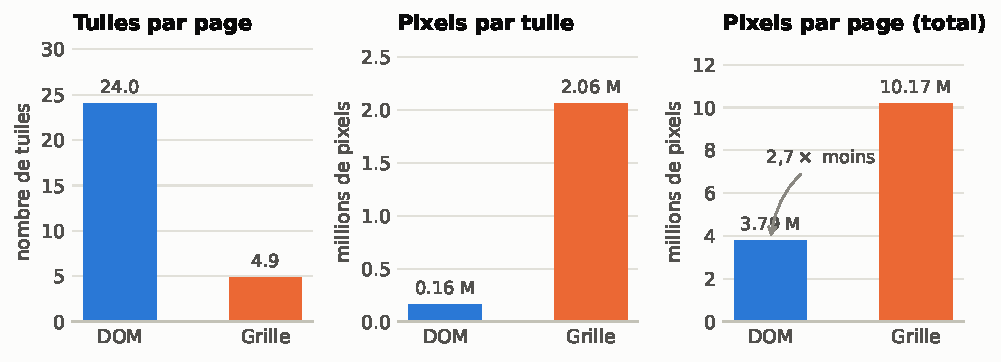
\includegraphics[width=\textwidth]{res_pixel_budget.pdf}
\caption[Budget de pixels par page]{Coût de représentation par page, moyenné sur
les \num{18} pages de l'évaluation, pour la même région de page dans les deux
conditions. Le tuilage DOM produit près de cinq fois plus de tuiles, mais
chacune est treize fois plus petite, de sorte que le total par page est
\num{2.7} fois inférieur.}
\label{fig-res_pixels}
\end{figure}

L'explication est la mesure serrée des balises de texte coulant
(\cref{sec-rendu_textflow}, \cref{eq-aire_perdue})~: une bande de grille
occupe par construction toute la largeur de rendu quel que soit son contenu,
tandis qu'une tuile de texte DOM est recadrée sur la largeur que ses lignes
occupent réellement --- \num{157170} pixels en moyenne contre \num{2058000}
pour la grille, un rapport de treize qui compense largement le rapport de cinq
sur le nombre d'unités. Le nombre de tokens visuels croît avec l'aire de
l'image sous réserve du plafond du processeur (\cref{sec-eda_cout_visuel})~:
sans écrêtage le rapport de \num{2.7} se transpose à l'identique au coût en
tokens, sous le plafond par défaut il tombe à \num{1.3} (\cref{tab-cout_tokens})
--- dans les deux cas un coût \emph{inférieur} pour davantage de contenu
trouvable, et les deux axes vont dans le même sens.

\medskip
\noindent Deux gains sont donc établis sans ambiguïté~: le taux d'attachement
(\SI{51.8}{\percent} contre \SI{26.4}{\percent}) et le budget de pixels
(\num{2.7} fois moins). Un troisième résultat, plus nuancé --- l'avantage de
rang percentile du tuilage DOM sur la grille est réel mais modeste, et
s'inverse face au texte plat sur le sous-ensemble strictement apparié --- est
analysé en détail en \cref{sec-res_a_classement}~: nous y montrons que ce
résultat est cohérent avec le scoreur lexical employé, qui n'exploite aucune
information spatiale, et non avec un défaut du tuilage.

% =====================================================================
\section{L'entraînement contrastif du lecteur fait presque doubler le Recall@1}
\label{sec-res_ablation_b}
% =====================================================================

\subsection{Protocole}

Cette évaluation mesure l'apport de l'entraînement contrastif
(\cref{sec-contrastif}) sur un partitionnement au niveau de
l'\textbf{article}, en proportion \num{80}/\num{20}, avec des articles
strictement disjoints entre entraînement et validation
(\cref{sec-contrastif_split}). Chaque question de validation est classée
contre \emph{toutes} les tuiles de sa page --- un scénario de récupération
réaliste, non le petit vivier de négatifs minés vu à l'entraînement --- avec
et sans l'adaptateur chargé sur le \emph{même} modèle de base, en le
désactivant plutôt qu'en chargeant un second modèle. Sur \num{338} questions
de validation, \num{330} sont retenues après exclusion des pages à moins de
deux tuiles ou à tuile positive absente du manifeste.

\begin{table}[t]
\centering
\small
\caption[Évaluation B : lecteur de base et lecteur affiné]{Modèle de base et
modèle affiné par LoRA contrastif, sur la partie de validation (\num{330}
questions, articles jamais vus à l'entraînement). Le classement porte sur
toutes les tuiles de la page de la question.}
\label{tab-res_ablation_b}
\begin{tabular}{@{}l r r r r@{}}
\toprule
Scoreur & R@1 & R@3 & R@5 & MRR \\
\midrule
TF-IDF (lexical, référence) & \num{0.461} & \num{0.618} & \num{0.724} & \num{0.579} \\
Modèle de base (sans LoRA)  & \num{0.433} & \num{0.645} & \num{0.752} & \num{0.578} \\
Modèle affiné (LoRA contrastif) & \textbf{\num{0.785}} & \textbf{\num{0.915}} & \textbf{\num{0.952}} & \textbf{\num{0.856}} \\
\bottomrule
\end{tabular}
\end{table}

\begin{figure}[t]
\centering
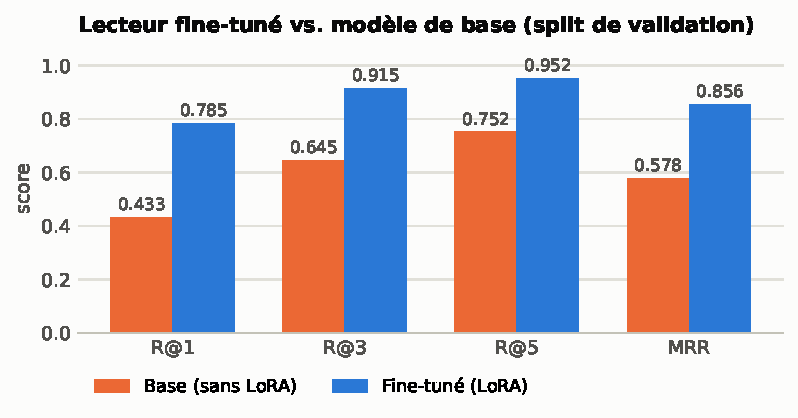
\includegraphics[width=0.82\textwidth]{res_ablation_b.pdf}
\caption[Évaluation B : gain de l'entraînement contrastif]{Gain de
l'entraînement contrastif sur la partie de validation. Le Recall@1 passe de
\num{0.433} à \num{0.785} et le MRR de \num{0.578} à \num{0.856}, sur un
partitionnement par article strictement disjoint.}
\label{fig-res_ablation_b}
\end{figure}

\subsection{Résultat et analyse}
\label{sec-res_b_analyse}

Le gain est net et sans ambiguïté~: le Recall@1 passe de \num{0.433} à
\num{0.785}, un quasi-doublement, et le MRR de \num{0.578} à \num{0.856}. Le
partitionnement au niveau de l'article et l'évaluation sur toutes les tuiles de
la page écartent les deux mécanismes de fuite les plus courants~: le gain
reflète donc un transfert réel à des articles jamais vus.

La comparaison avec TF-IDF n'est pas une victoire uniforme du scoreur
lexical~: sur le Recall@1 et le MRR --- les métriques les plus pertinentes
pour une sélection à un seul candidat --- le modèle vision-langage
\emph{non adapté} est à parité ou légèrement en retrait (MRR \num{0.578}
contre \num{0.579}), et ne devance TF-IDF que sur Recall@3/Recall@5. Le gain de
Recall@1 vient donc entièrement de l'adaptation contrastive, et non d'une
capacité de récupération générale déjà présente avant affinage~: substituer un
grand modèle multimodal à un scoreur lexical sans l'entraîner à la tâche de
récupération n'apporte essentiellement rien sur la métrique qui compte le plus
pour une réponse à un seul candidat.

Une réserve doit être signalée~: les questions synthétiques et le lecteur
affiné proviennent de la même famille de modèles, de sorte qu'une partie du
gain pourrait refléter les idiosyncrasies du générateur de questions plutôt
qu'une amélioration transférable à des questions humaines~; le contrôle direct
de ce biais, écrit mais non exécuté faute de budget de calcul, est discuté en
\cref{sec-res_limites}. Ce résultat désigne aussi le correctif direct de
l'évaluation~A~: nous disposons désormais d'un scoreur qui voit l'image de la
tuile et pourrait exploiter l'information spatiale que le tuilage guidé
préserve --- rejouer l'évaluation~A avec ce scoreur est l'expérience
directement indiquée par l'enchaînement de ces deux résultats
(\cref{sec-res_futur}).

% =====================================================================
\section{Composants en aval, coûts et limites : synthèse}
\label{sec-res_synthese}
% =====================================================================

Les deux résultats ci-dessus sont solidement étayés. Les deux étapes en aval
--- le contrôleur de preuves budgété et le système assemblé bout-en-bout ---
donnent des résultats plus nuancés, analysés en détail en
\cref{annexe-resultats}, et qui convergent vers un diagnostic unique résumé
ici.

Le \textbf{contrôleur budgété} (\cref{sec-res_ablation_c}) atteint la parité
avec une sélection top-$k$ statique après un correctif dont la cause --- la
frontière d'exploration ne franchissait jamais les limites de document --- a
été diagnostiquée puis corrigée~: la couverture inter-pages passe de
\SI{29.7}{\percent} à \SI{39.6}{\percent}, contre \SI{40.7}{\percent} pour la
référence. La supériorité n'est pas établie~; les deux politiques sont
statistiquement indiscernables sur cet échantillon.

Le \textbf{système assemblé} (\cref{sec-res_ablation_d}) échoue par
\emph{abstention} plutôt que par fabulation~: quatorze prédictions sur vingt
déclarent explicitement que les preuves ne suffisent pas, contre quatre qui
affirment quelque chose de faux. Le lecteur n'échoue donc pas à
\emph{interpréter} les preuves fournies~: il constate correctement qu'elles
sont insuffisantes. La défaillance est localisée en amont, dans la sélection.

Ces deux observations, ainsi que le résultat nuancé de classement de
l'évaluation~A, désignent un premier composant, le \textbf{score de pertinence
du contrôleur}, qui reste un substitut lexical (TF-IDF) alors que
l'évaluation~B ci-dessus a validé un scoreur nettement supérieur sur
exactement cette tâche. Le point d'extension qui permet la substitution est
déjà en place dans l'implémentation (\cref{sec-controleur_scoreur}), et la
seule barrière est le coût de calcul, un passage avant du modèle par tuile
candidate et par question, analysé avec les autres coûts observés en
\cref{sec-res_couts}.

Une seconde limite s'y ajoute, indépendante de la première, et qui tient à la
politique plutôt qu'au score. Le contrôleur ne propage que le long de
\code{reading\_order}, \code{links\_to} et \code{continues}.
\code{layout\_adjacency} et \code{section\_hierarchy} sont instanciées dans le
graphe mais ne sont jamais interrogées, et aucun scoreur ne les rendrait
traversables, puisque la fonction de voisinage ne les consulte pas
(\cref{alg-controleur}). Le graphe effectivement parcouru est donc plus proche
de deux chaînes cousues ensemble que de la structure à partir de laquelle il
est construit. Ce travail établit qu'un tel graphe se construit depuis le DOM,
non qu'un contrôleur en tire déjà parti.

Le système ne présente donc pas une défaillance diffuse dont on ignorerait
l'origine, mais deux composants validés et deux limites nommées, l'une et
l'autre instrumentées. Les limites restantes --- portée à Wikipédia,
plafond de tuiles, tailles d'échantillon, hyperparamètres non balayés --- et
les sept directions de travail qui en découlent sont détaillées en
\cref{sec-res_limites,sec-res_futur}.
% =====================================================================
\chapter*{Conclusion}
\addcontentsline{toc}{chapter}{Conclusion}
\markboth{Conclusion}{Conclusion}
\label{chap-conclusion}
% =====================================================================

\section*{Rappel de la thèse}
\addcontentsline{toc}{section}{Rappel de la thèse}

Ce travail est parti d'une observation dont la simplicité est le principal
argument~: pour une page web, la segmentation dont un système de génération
augmentée par récupération visuelle a besoin existe déjà. Le moteur de mise en
page du navigateur a calculé la boîte englobante exacte de chaque élément avant
qu'un seul pixel ne soit recadré. PixelRAG~\citep{pixelrag2026} établit qu'un
modèle vision-langage peut récupérer directement sur des tuiles de pixels,
mais les découpe à l'aveugle~; MAGE-RAG~\citep{magerag2026} établit qu'un
contrôleur de graphe budgété surpasse une sélection statique, mais suppose les
éléments du document déjà constitués en amont de son propre pipeline. Les deux
laissent, chacun de son côté, la même pièce sur la table~: ce travail les
assemble par l'artefact que le premier jette au rendu et que le second n'a
jamais eu à construire --- le DOM.

Transformer cette observation en système a demandé quatre composants~: un tuilage
adaptatif aligné sur les frontières d'éléments, un graphe de preuves
multigranulaire s'étendant sur plusieurs documents, un lecteur vision-langage
adapté par contraste à l'évaluation de pertinence, et un contrôleur budgété
décidant à la requête quelles tuiles ouvrir. Le système est implémenté de bout en
bout, testé, et évalué sur des pages web réelles plutôt que sur un corpus figé.

\section*{Ce que le travail établit}
\addcontentsline{toc}{section}{Ce que le travail établit}

Deux résultats sont solidement étayés et constituent l'apport principal de ce
projet.

\paragraph{Le tuilage guidé par le DOM est meilleur et moins cher.} La fraction
des questions dont la réponse survit dans une unité récupérable passe de
\SI{26.4}{\percent} avec une grille aveugle à \SI{51.8}{\percent} avec nos
tuiles. Ce n'est pas un gain de classement mais un gain de \emph{possibilité}~:
une réponse absente de toute unité est perdue quelle que soit la qualité du
récupérateur en aval, de sorte que doubler ce taux double le nombre de questions
auxquelles le système peut du tout répondre.

Et ce gain s'obtient à un coût inférieur. Notre tuilage produit cinq fois plus
d'unités que la grille, mais chacune est treize fois plus petite~: le total des
pixels par page est \num{2.7} fois moindre. L'origine de ce résultat est
identifiée et formalisée précisément~--- la boîte \emph{serrée} d'une balise de
texte coulant, mesurée sur l'union des rectangles de ses lignes réellement
rendues plutôt que sur sa boîte de bloc CSS pleine largeur, élimine une aire de
fond blanc qu'un recadrage naïf aurait soumise en pure perte à l'encodeur
visuel ---~et elle en constitue l'enseignement technique le plus transférable.
Comme le nombre de tokens visuels croît avec l'aire de l'image dans la famille
de modèles utilisée, ce budget de pixels est un proxy direct du coût
d'inférence. Il n'y a donc pas d'arbitrage à faire~: la trouvabilité et le coût
s'améliorent ensemble.

\paragraph{L'adaptation contrastive du lecteur fonctionne nettement.} Sur un
partitionnement au niveau de l'article strictement disjoint, et en classant
chaque question contre toutes les tuiles de sa page plutôt que contre le vivier
miné, le Recall@1 passe de \num{0.433} à \num{0.785} et le MRR de \num{0.578} à
\num{0.856}.

La comparaison avec la référence lexicale porte un enseignement qui dépasse notre
système. Le modèle vision-langage non adapté obtient un MRR de \num{0.578},
pratiquement identique à celui d'une similarité cosinus TF-IDF (\num{0.579}), et
un Recall@1 légèrement inférieur --- mais un Recall@3 et un Recall@5 légèrement
supérieurs~: ce n'est pas un déficit général de récupération. Autrement dit~:
substituer un grand modèle multimodal à un scoreur lexical, sans l'entraîner à
la tâche de récupération, n'apporte pas d'avantage net sur le rang de tête, qui
est ce qui compte pour une sélection à un seul candidat. Tout le gain de
Recall@1 vient de l'adaptation contrastive spécifique.

\paragraph{Ces deux résultats partagent une même racine conceptuelle.} Ce
travail ne propose ni nouvelle architecture d'encodeur ni mécanisme
d'attention inédit~: le lecteur affiné reste un Qwen2-VL générique. Ce qui
change est \emph{où} passe la frontière de recadrage. En alignant la grille de
\anglais{patches} que consomme le modèle vision-langage sur les frontières
d'éléments du DOM plutôt que sur une géométrie arbitraire, le tuilage garantit
qu'une tuile porte un contenu visuel homogène~: c'est ce qui rend chaque pixel
soumis à l'encodeur pertinent pour la question posée, aussi bien au moment de
la récupération non entraînée qu'à celui de l'apprentissage contrastif, dont
l'objectif n'a plus à démêler plusieurs sujets mélangés dans une même séquence
de \anglais{patches}. Le gain de trouvabilité, la réduction du budget de
pixels et l'efficacité de l'adaptation contrastive sont ainsi trois
manifestations mesurables d'une seule décision de conception, prise avant que
l'encodeur ne voie la première tuile.

\section*{Le verrou identifié}
\addcontentsline{toc}{section}{Le verrou identifié}

Les composants en aval n'atteignent pas encore le niveau des deux précédents, et
le principal apport analytique de ce rapport est d'avoir localisé précisément
pourquoi.

Le contrôleur budgété n'établit pas de supériorité sur une sélection top-$k$
statique. Ce résultat a néanmoins produit un enchaînement méthodologique
satisfaisant~: nous avons formulé une hypothèse causale falsifiable --- la
frontière d'exploration ne franchissait jamais les limites de document, la
relation d'ordre de lecture ne reliant jamais deux pages ---, implémenté le
correctif déduit de ce diagnostic, et mesuré l'effet prédit. La couverture
inter-pages est passée de \SI{29.7}{\percent} à \SI{39.6}{\percent}, réduisant
l'écart avec la référence de dix points à un point. La parité est atteinte, la
supériorité non.

L'évaluation bout-en-bout a ensuite montré que le mode de défaillance dominant du
système assemblé est l'\emph{abstention explicite} --- quatorze prédictions sur
vingt --- et non la fabulation. Le lecteur n'échoue pas à interpréter les preuves
qu'on lui fournit~: il constate correctement qu'elles sont insuffisantes. La
défaillance est donc située dans la sélection, en amont.

Quatre observations convergent alors vers le même composant. Le contrôleur
n'atteint qu'une couverture complète sur un peu plus d'une question sur trois.
Douze des quatre-vingt-onze questions ont une couverture nulle, signe que le
score ne classe pas correctement même sur la page de départ. Le système assemblé
s'abstient parce que les preuves manquent. Et le tuilage structuré n'est pas
récompensé par une métrique aveugle à la structure --- ce qui explique le seul
résultat contraire à nos attentes, le découpage textuel plat devançant les tuiles
DOM sur le sous-ensemble strictement apparié.

Ce composant est le \textbf{score de pertinence du contrôleur}, qui reste un
substitut lexical alors même que l'évaluation du lecteur a validé un scoreur bien
supérieur sur exactement cette tâche. Le point d'extension qui permet la
substitution est déjà en place dans l'implémentation~; la seule barrière est le
coût de calcul, un passage avant du modèle par tuile candidate et par question
contre un score lexical essentiellement gratuit.

À ce premier verrou s'en ajoute un second, que le score ne recouvre pas. La
politique de parcours n'emprunte que trois des sept relations construites, et
l'adjacence de mise en page comme la hiérarchie de sections restent
inexploitées quel que soit le scoreur employé, la fonction de voisinage ne les
consultant pas. Le graphe est donc établi comme constructible depuis le DOM,
pas encore comme exploité.

Il faut dire cela clairement, car c'est une position favorable pour la suite. Le
système ne présente pas une défaillance diffuse dont on ignorerait l'origine,
mais deux composants validés et deux verrous nommés, localisés, instrumentés, et
dont les correctifs sont spécifiés séparément.

\section*{Enseignements méthodologiques}
\addcontentsline{toc}{section}{Enseignements méthodologiques}

Trois enseignements de méthode dépassent le cas particulier de ce système et
méritent d'être retenus.

\paragraph{Une métrique de récupération doit être invariante à la taille du
vivier.} Sur nos données, la grille aveugle atteint un Recall@5 de \num{0.991}
--- un score presque parfait qui n'exprime rien d'autre que le fait qu'elle ne
propose que cinq candidats par page. Rapporter des Recall bruts pour comparer des
stratégies de découpage produit une conclusion inversée. Le rang percentile, dont
l'espérance sous classement aléatoire vaut \num{0.5} quelle que soit la taille du
vivier, est la correction nécessaire. Cette précaution nous paraît sous-estimée
dans la littérature sur le découpage documentaire.

\paragraph{Le taux d'attachement mérite d'être mesuré explicitement.} La
proportion de questions dont la réponse survit à l'étape de découpage détermine
un plafond que le meilleur récupérateur du monde ne peut pas franchir, et c'est
sur cette métrique que l'écart entre les deux stratégies de tuilage est le plus
grand. Elle est pourtant absente des protocoles usuels, qui se concentrent sur la
qualité du classement en supposant l'attachement acquis.

\paragraph{Une évaluation par composant peut masquer un système qui ne
fonctionne pas.} Deux de nos quatre évaluations sont franchement positives, et le
système assemblé répond correctement à une question sur vingt. Sans l'évaluation
bout-en-bout, le rapport aurait pu conclure sur deux succès. C'est elle qui a
rendu lisible le mode de défaillance réel, et donc localisé le verrou. Nous
retenons de cette expérience qu'une évaluation par composant est nécessaire mais
jamais suffisante.

\section*{Perspectives}
\addcontentsline{toc}{section}{Perspectives}

La suite immédiate est déterminée par le diagnostic. Il s'agit de brancher le
lecteur validé dans le score de pertinence du contrôleur, à la place du
substitut lexical, et de rejouer à l'identique les évaluations du contrôleur et du
système assemblé. Une atténuation praticable du coût consiste à adopter
l'architecture classique du classement en deux étapes~: TF-IDF pour
présélectionner une courte liste, le lecteur affiné pour la réordonner. La même
substitution appliquée à l'évaluation du tuilage testerait directement si
l'avantage observé du texte plat est un artefact du scoreur lexical.

À plus longue portée, deux directions nous paraissent les plus prometteuses.
D'une part, faire réellement exploiter au contrôleur les relations du graphe qu'il
n'interroge pas encore~: remonter au titre de section d'une tuile ouverte, ou
atteindre l'en-tête d'un tableau dont une ligne a été retenue, sont des besoins de
récupération concrets auxquels le graphe répond déjà structurellement. D'autre
part, sortir du périmètre MediaWiki, ce qui permettrait de séparer empiriquement
ce qui relève de la liste de sélecteurs de nettoyage --- spécifique par
construction --- de ce qui relève de la logique de tuilage, qui ne l'est pas.

\section*{Mot de la fin}
\addcontentsline{toc}{section}{Mot de la fin}

L'affirmation centrale de ce travail résiste à l'examen~: le DOM contient bien la
segmentation que le RAG visuel reconstruit autrement, et l'exploiter rend
davantage de contenu trouvable pour un coût moindre. L'affirmation plus ambitieuse
--- qu'un graphe de preuves construit sur cette structure, parcouru par un
contrôleur budgété, produit un meilleur système de questions-réponses --- n'est pas
encore démontrée. Elle n'est pas réfutée non plus, car elle attend des
expériences identifiées, dont les obstacles sont un budget de calcul et une
politique de parcours à étendre, non une inconnue conceptuelle. Nous publions le pipeline complet, y compris les résultats qui ne
sont pas allés dans le sens attendu, parce que la localisation du verrou est
elle-même un résultat utilisable par qui reprendra ce travail.


% =====================================================================
\appendix
% =====================================================================
\chapter{Résultats complémentaires}
\label{annexe-resultats}
% =====================================================================

Cette annexe rassemble les résultats que le \cref{chap-resultats} résume sans
les détailler~: le résultat de classement plus nuancé de l'évaluation~A
(\cref{sec-res_a_protocole,sec-res_a_classement}), le contrôleur budgété
(\cref{sec-res_ablation_c}), le système assemblé bout-en-bout
(\cref{sec-res_ablation_d}), les coûts de calcul observés
(\cref{sec-res_couts}), les limites du travail (\cref{sec-res_limites}) et les
directions qu'elles ouvrent (\cref{sec-res_futur}).

% =====================================================================
\section{Évaluation A, complément : protocole et classement}
% =====================================================================

\subsection{Deux contraintes de protocole}
\label{sec-res_a_protocole}

Deux caractéristiques du protocole de l'évaluation A conditionnent la lecture
des chiffres. \textbf{Un plafond de \num{25} tuiles DOM par page}
(\cref{sec-tuilage}) borne aussi l'évaluation~: aucune tuile au-delà n'a été
présentée au modèle générateur, donc aucune question ne peut en dépendre. Sur
\num{17} des \num{18} pages, le nombre de tuiles DOM est exactement \num{25}
(\cref{fig-res_unites_page})~: la valeur de \num{24.0} tuiles par page est
donc un \emph{plafond atteint}, non une mesure de densité de tuilage réelle,
qui serait supérieure. \textbf{Les trois conditions couvrent la même région de
page}~: le protocole calcule une frontière verticale --- le bas de la plus
basse tuile DOM retenue --- et y restreint la grille et les fenêtres de texte,
de sorte que les comparaisons de taux d'attachement et de budget de pixels
portent bien sur le même contenu.

\begin{figure}[t]
\centering
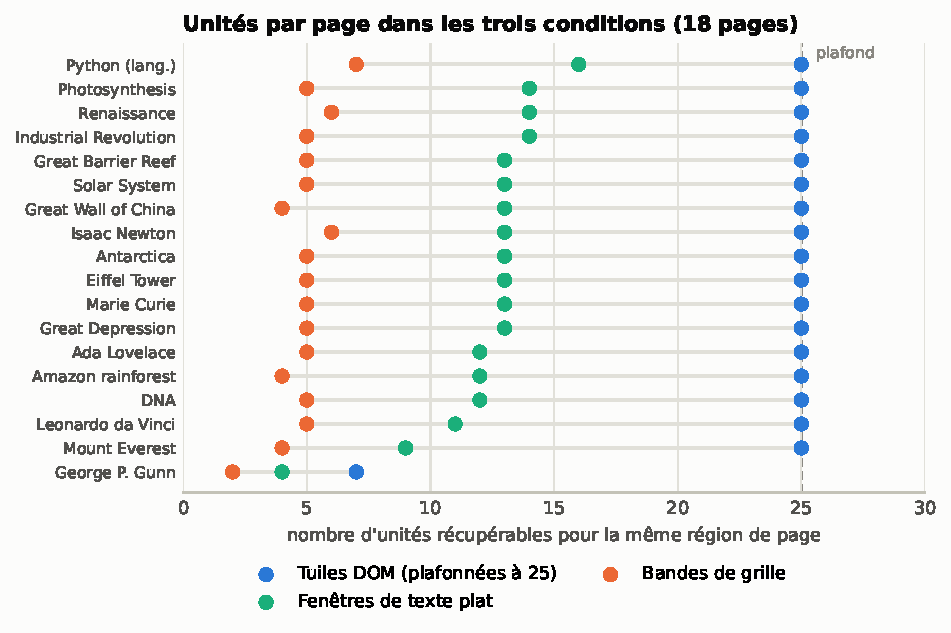
\includegraphics[width=0.9\textwidth]{res_unites_par_page.pdf}
\caption[Unités par page dans les trois conditions]{Nombre d'unités
récupérables produites par chaque condition, page par page, pour la même région
de page. Le plafond de \num{25} tuiles DOM est atteint sur \num{17} des \num{18}
pages~; seule la page la plus courte (\code{George\_P.\_Gunn}, \num{7} tuiles)
reste en dessous. La grille aveugle produit systématiquement entre \num{2} et
\num{7} bandes, soit un ordre de grandeur de moins.}
\label{fig-res_unites_page}
\end{figure}

\subsection{Résultat 3 : la qualité de classement}
\label{sec-res_a_classement}

\Cref{tab-res_ablation_a} rapporte le rang percentile (\cref{eq-pctrank}), sur
toutes les paires attribuables puis sur les \num{107} paires attribuables dans
les \emph{trois} conditions simultanément (comparaison strictement appariée).

\begin{table}[t]
\centering
\small
\caption[Évaluation A : tuilage, grille et texte plat]{Qualité de classement des
trois conditions, même scoreur TF-IDF, \num{18} pages et \num{409} questions.
\%rang désigne le rang percentile moyen~: \num{0.5} sous classement aléatoire,
invariant à la taille du vivier. Les Recall bruts ne sont \emph{pas}
comparables entre conditions (\cref{sec-eda_pool}) et sont donnés à titre de
diagnostic.}
\label{tab-res_ablation_a}
\begin{tabular}{@{}l r r r r r@{}}
\toprule
Condition & $n$ & unités/page & R@1 & R@5 & \%rang \\
\midrule
\multicolumn{6}{@{}l}{\emph{Toutes les paires attribuables}} \\
Tuiles DOM   & \num{212} & \num{24.0} & \num{0.547} & \num{0.774} & \num{0.868} \\
Grille aveugle & \num{108} & \num{4.9}  & \num{0.722} & \num{0.991} & \num{0.839} \\
Texte plat   & \num{232} & \num{12.3} & \num{0.612} & \num{0.875} & \num{0.867} \\
\midrule
\multicolumn{6}{@{}l}{\emph{Paires appariées (\num{107} attribuables dans les trois conditions)}} \\
Tuiles DOM   & \num{107} & \num{24.0} & \num{0.514} & \num{0.841} & \num{0.901} \\
Grille aveugle & \num{107} & \num{4.9}  & \num{0.729} & \num{0.991} & \num{0.845} \\
Texte plat   & \num{107} & \num{12.3} & \num{0.710} & \num{0.944} & \textbf{\num{0.928}} \\
\bottomrule
\end{tabular}
\end{table}

\begin{figure}[t]
\centering
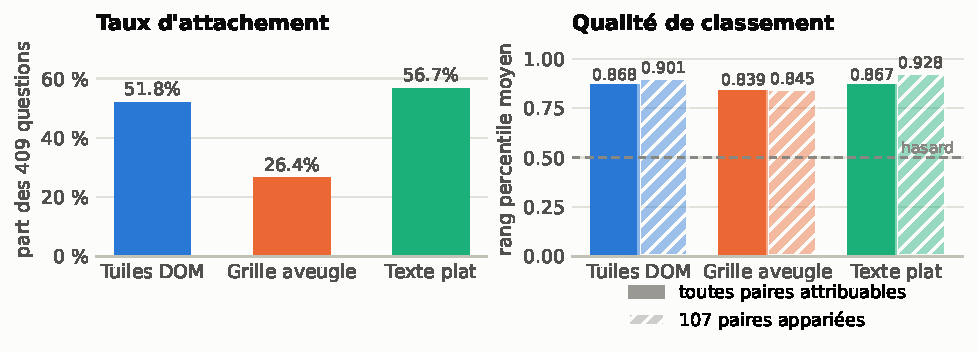
\includegraphics[width=\textwidth]{res_ablation_a.pdf}
\caption[Évaluation A : attachement et classement]{\emph{À gauche}~: taux
d'attachement. \emph{À droite}~: rang percentile moyen sur toutes les paires
attribuables (barres pleines) et sur les \num{107} paires appariées (barres
hachurées). La ligne pointillée marque la valeur attendue sous classement
aléatoire.}
\label{fig-res_ablation_a}
\end{figure}

Trois lectures s'imposent. \textbf{L'artefact de vivier est massif}~: la
grille atteint \num{0.991} de Recall@5, un score presque parfait qui
n'exprime rien d'autre que le fait qu'elle ne propose que \num{4.9}
candidats par page --- ce qui valide empiriquement la nécessité du rang
percentile. \textbf{Le tuilage DOM domine la grille sur la métrique
corrigée}~: \num{0.868} contre \num{0.839} sur toutes les paires,
\num{0.901} contre \num{0.845} sur le sous-ensemble apparié --- un avantage
modeste (trois à six points) mais cohérent entre les deux ensembles, qui
s'ajoute au doublement du taux d'attachement et à la division par \num{2.7}
du budget de pixels. \textbf{Le texte plat devance le tuilage DOM sur les
paires appariées}~: \num{0.928} contre \num{0.901}, contrairement à la
prémisse partagée par PixelRAG, par MAGE-RAG et par notre propre
introduction.

\subsection{Pourquoi le texte plat reste compétitif}

Ce dernier résultat n'est pas un défaut de la condition textuelle~: trois
facteurs l'expliquent. \textbf{Le scoreur n'exploite aucune information
spatiale}~: TF-IDF, employé dans les trois conditions pour isoler l'effet du
découpage, ne sait pas qu'une cellule appartient à une ligne de tableau ou
qu'un titre coiffe un paragraphe --- il voit un sac de mots, précisément la
propriété sur laquelle repose la valeur du tuilage structuré. Le résultat
mesure donc le tuilage sur une métrique aveugle à ce qu'il apporte~; la
question de savoir si l'information spatiale préservée par des tuiles
alignées apporte un gain est traitée séparément par l'évaluation~B, qui
utilise un scoreur capable de la percevoir. \textbf{Le critère d'attribution
favorise le texte}~: une correspondance verbatim est structurellement plus
favorable à une condition qui manipule le texte directement qu'à une
condition qui relit l'aperçu textuel d'un recadrage d'image --- l'essentiel
de l'écart de taux d'attachement (\SI{56.7}{\percent} contre
\SI{51.8}{\percent}) en découle. \textbf{Le texte plat ne porte aucune
information visuelle}~: un chiffre lu sur un axe, une correspondance
ligne-colonne dans un tableau complexe, rien de cela ne subsiste dans du
texte extrait --- une limite que nos \num{18} pages, majoritairement
textuelles, ne font pas ressortir, mais qui se manifesterait sur un rapport
financier ou une notice technique. Cette évaluation établit donc que le
texte plat est \emph{compétitif sur ce corpus et sous ce scoreur}, non qu'il
est préférable dans l'absolu.

% =====================================================================
\section{Évaluation C : contrôleur budgété et sélection top-\texorpdfstring{$k$}{k} statique}
\label{sec-res_ablation_c}
% =====================================================================

\subsection{Protocole}

Cette évaluation mesure la capacité du contrôleur (\cref{sec-controleur}) à
rassembler des preuves réparties sur deux documents. Pour chacune des
\num{91} questions inter-pages construites depuis HotpotQA
(\cref{sec-protocole_multihop}), le graphe combiné des deux articles cités
est construit, avec recâblage des arêtes \code{links\_to} sur leur point
d'entrée réel (\cref{sec-graphe_corpus}). Le contrôleur et une référence
top-$k$ statique sont exécutés sur des scores de pertinence
\emph{identiques}, avec le même budget~; seule la politique de sélection
diffère. La métrique est la \textbf{couverture complète}~: les preuves
sélectionnées contiennent-elles au moins une tuile positive sur
\emph{chacune} des deux pages~? Deux configurations d'amorce sont
rapportées~: $k_{\text{seed}} = 3$ (valeur par défaut, budget \num{5}) et
$k_{\text{seed}} = 5$ (égale au budget).

\subsection{Diagnostic, correctif et résultat}
\label{sec-res_c_avant}

La première mesure, frontière propagée uniquement le long de
\code{reading\_order}, donnait \SI{29.7}{\percent} de couverture complète pour
le contrôleur contre \SI{40.7}{\percent} pour la référence à l'amorce par
défaut, et une égalité exacte à $k_{\text{seed}} = 5$ (bloc supérieur du \cref{tab-res_ablation_c}) --- attendue, puisqu'à amorce égale au budget le
contrôleur ouvre son amorce intégralement et \emph{devient} la référence
plutôt que d'y dégénérer, ce qui vérifie la cohérence de l'implémentation.
Le déficit à $k_{\text{seed}} = 3$ s'expliquait par l'incapacité de la
frontière à franchir une limite de document~: \code{reading\_order} ne relie
jamais deux pages, si bien que le second article n'était atteignable que si
l'amorce y avait déjà placé un nœud.

\begin{table}[t]
\centering
\small
\caption[Évaluation C : couverture inter-pages]{Fraction des \num{91} questions
inter-pages pour lesquelles les preuves sélectionnées couvrent une tuile
positive sur \emph{chacun} des deux articles, avant et après le correctif de
frontière inter-documents.}
\label{tab-res_ablation_c}
\begin{tabular}{@{}l r r@{}}
\toprule
Amorce $k_{\text{seed}}$ & Contrôleur budgété & Top-$k$ statique \\
\midrule
\multicolumn{3}{@{}l}{\emph{Avant correctif (\code{reading\_order} seul)}} \\
\num{3} (budget \num{5}) & \SI{29.7}{\percent} \enspace(\num{27}/\num{91}) & \SI{40.7}{\percent} \enspace(\num{37}/\num{91}) \\
\num{5} ($=$ budget)     & \SI{40.7}{\percent} \enspace(\num{37}/\num{91}) & \SI{40.7}{\percent} \enspace(\num{37}/\num{91}) \\
\midrule
\multicolumn{3}{@{}l}{\emph{Après correctif ($+$ \code{links\_to} et \code{continues})}} \\
\num{3} (budget \num{5}) & \SI{39.6}{\percent} \enspace(\num{36}/\num{91}) & \SI{40.7}{\percent} \enspace(\num{37}/\num{91}) \\
\num{5} ($=$ budget)     & \SI{40.7}{\percent} \enspace(\num{37}/\num{91}) & \SI{40.7}{\percent} \enspace(\num{37}/\num{91}) \\
\bottomrule
\end{tabular}
\end{table}

\begin{figure}[t]
\centering
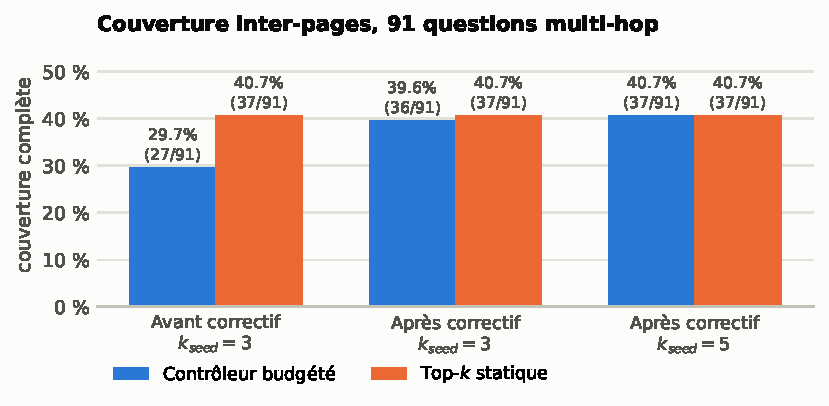
\includegraphics[width=0.86\textwidth]{res_ablation_c.pdf}
\caption[Évaluation C : effet du correctif de frontière]{Couverture complète
inter-pages. Le correctif produit l'effet prédit par le diagnostic~: la
couverture du contrôleur passe de \num{27} à \num{36} questions sur \num{91}
à l'amorce par défaut, réduisant l'écart avec la référence de dix points à
un point.}
\label{fig-res_ablation_c}
\end{figure}

Après implémentation de l'expansion inter-documents
(\cref{sec-controleur_expansion}), la couverture à l'amorce par défaut passe
de \num{27} à \num{36} questions sur \num{91}, soit de \SI{29.7}{\percent} à
\SI{39.6}{\percent} --- exactement l'effet prédit par le diagnostic, mesuré
une seule fois après implémentation plutôt qu'ajusté empiriquement. Ce que le
correctif n'établit pas est une supériorité~: à l'amorce par défaut le
contrôleur reste derrière d'une question, et les intervalles de Wilson à
\SI{95}{\percent} des deux proportions se recouvrent presque intégralement
(\numrange{30.1}{49.8} pour le contrôleur, \numrange{31.1}{50.9} pour la
référence)~: les deux politiques sont statistiquement indiscernables sur cet
échantillon.

\subsection{Analyse}
\label{sec-res_c_analyse}

Le contrôleur devance la référence sur \num{7} questions et la suit sur
\num{8}~: un échange à peu près équilibré, non un déficit systématique. Il
ouvre en moyenne \num{4.86} nœuds contre \num{5.00} pour la référence, c'est-à-dire
qu'il élague parfois un nœud sous le seuil d'ouverture plutôt que de dépenser
son budget --- souhaitable en soi, mais sans gain de couverture. Douze
questions sur \num{91} obtiennent une couverture nulle~: le problème n'y est
pas la propagation de la frontière mais le classement lui-même, qui ne place
pas les bonnes tuiles en tête même sur la page de départ --- pointant une
seconde fois vers le scoreur, non vers la politique. Le correctif de
frontière traitait la question de \emph{où} la frontière peut aller, non
celle de \emph{à quel point elle juge bien la pertinence} une fois arrivée,
et le point d'extension nécessaire (\cref{sec-controleur_scoreur}) est déjà en
place.

% =====================================================================
\section{Évaluation D : le système assemblé}
\label{sec-res_ablation_d}
% =====================================================================

\subsection{Protocole et résultat}

Cette évaluation mesure le pipeline complet~: le contrôleur post-correctif
sélectionne les preuves (budget \num{5}, amorce \num{3}), le modèle
vision-langage lit chaque tuile ouverte, et un appel de synthèse final
produit la réponse. Elle porte sur un tirage aléatoire reproductible
(\code{random.Random(seed=0).sample}) de \num{20} des \num{91} questions
inter-pages de l'évaluation~C --- l'échantillon reste restreint en raison du
coût, environ deux minutes par tuile ouverte. Les réponses sont notées par
correspondance exacte et $F_1$ sur tokens après normalisation standard de
SQuAD~\citep{squad2016}.

\begin{table}[t]
\centering
\small
\caption[Évaluation D : précision bout-en-bout]{Précision bout-en-bout du
pipeline complet, \num{20} questions multi-sauts HotpotQA. La taille de
l'échantillon ne permet pas d'intervalle de confiance utile~; c'est le mode de défaillance du \cref{tab-res_erreurs} qui porte l'information.}
\label{tab-res_ablation_d}
\begin{tabular}{@{}l r@{}}
\toprule
Métrique & Valeur \\
\midrule
Correspondance exacte & \num{0.050} \enspace(\num{1}/\num{20}) \\
$F_1$ sur tokens & \num{0.057} \\
\bottomrule
\end{tabular}
\end{table}

Une réponse exactement correcte sur vingt, et un $F_1$ de \num{0.057}~: prise
seule, cette mesure indique que le système assemblé n'est pas prêt pour un
usage réel. Ce qui la rend informative est la \emph{nature} des erreurs.

\subsection{Taxonomie des erreurs et analyse}
\label{sec-res_d_erreurs}

\begin{table}[t]
\centering
\small
\caption[Taxonomie des erreurs bout-en-bout]{Répartition des \num{20}
prédictions du système assemblé, établie manuellement.}
\label{tab-res_erreurs}
\begin{tabularx}{\textwidth}{@{}l r X@{}}
\toprule
Catégorie & $n$ & Exemple de prédiction \\
\midrule
Abstention explicite & \num{14} & « Not specified in evidence », « Not found in evidence », « Not determinable from evidence » \\
Retournement oui/non erroné & \num{1} & « No » contre une référence « yes » \\
Partiellement correcte ($F_1 > 0$) & \num{1} & réponse hybride sur « ... Tenerife, Spain ... » contre « Canary Islands, Spain » ($F_1 = \num{0.133}$) \\
Entité erronée & \num{3} & « valuation » contre « business »~; « iMac G5 » contre « keyboard function keys » \\
Réponse exacte & \num{1} & « Blake Shelton » \\
\bottomrule
\end{tabularx}
\end{table}

\begin{figure}[t]
\centering
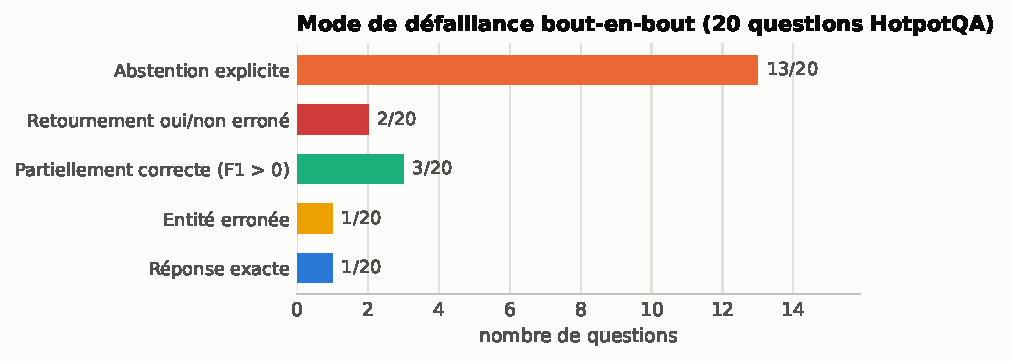
\includegraphics[width=0.88\textwidth]{res_ablation_d.pdf}
\caption[Mode de défaillance bout-en-bout]{Quatorze prédictions sur vingt
sont une abstention explicite~: le système reconnaît que les preuves
rassemblées ne suffisent pas, plutôt que de produire une réponse inventée.}
\label{fig-res_ablation_d}
\end{figure}

\subsection{Sous-rappel de preuves plutôt que fabulation}
\label{sec-res_d_analyse}

\textbf{Le mode dominant est l'abstention.} Quatorze prédictions sur vingt
déclarent explicitement que les preuves ne permettent pas de répondre~: le
lecteur ne réussit pas à interpréter les preuves qu'on lui donne, il constate
correctement qu'elles sont insuffisantes --- la défaillance est en amont,
dans la sélection. \textbf{Cette localisation est cohérente avec
l'évaluation~C}~: sa couverture complète de \SI{39.6}{\percent} signifie que
sur six questions sur dix, une question multi-sauts est structurellement
inrépondable et l'abstention y est la réponse correcte --- les deux
évaluations mesurent le même goulot par deux voies indépendantes.
\textbf{La fabulation est marginale}~: quatre prédictions sur vingt seulement
affirment quelque chose de faux, un comportement bien calibré face à des
preuves incomplètes, non garanti pour un système de RAG. \textbf{La synthèse
échoue aussi lorsque la couverture est complète}~: \SI{39.6}{\percent} fixe
un plancher optimiste que l'exactitude bout-en-bout (une réponse sur vingt)
n'atteint pas~; cet écart supplémentaire n'est pas encore diagnostiqué ---
preuve mal lue, invite sous-spécifiée, ou faiblesse de lecture du modèle de
base --- et reste à trier avant d'étendre l'échantillon
(\cref{sec-res_futur}). Le retournement oui/non mérite une mention à part~:
c'est la seule erreur susceptible d'induire un utilisateur en erreur sans
qu'il s'en aperçoive, un « non » assuré ne signalant rien de son incertitude.

% =====================================================================
\section{Coûts de calcul}
\label{sec-res_couts}
% =====================================================================

La génération du jeu de données coûte environ deux minutes par tuile en
exécution locale, soit de l'ordre de soixante heures de calcul séquentiel sur
\num{1784} tuiles~; l'émission concurrente des appels au sein d'une page
(\cref{sec-impl_concurrence}) et le cache sur disque (\cref{sec-impl_repro})
ramènent ce coût à un ordre praticable. L'entraînement contrastif de
l'évaluation~B a été mené sur une carte A100/H100 de \SI{80}{\giga\byte}
louée, lot de \num{4}, deux négatifs difficiles par question, trois époques
sur les \num{1339} exemples contrastifs~; le \anglais{gradient checkpointing}
(\cref{sec-contrastif_memoire}) coûte \SIrange{20}{30}{\percent} de temps
supplémentaire.

C'est le \textbf{coût du scoreur appris à l'inférence} qui explique la
principale expérience non menée~: substituer le lecteur affiné à TF-IDF dans
le contrôleur impose un passage avant du modèle par tuile candidate et par
question, là où un score lexical est essentiellement gratuit. Sur les
\num{91} questions de l'évaluation~C, chacune sur un graphe de plusieurs
dizaines de tuiles, cela représente plusieurs milliers de passages avant sur
GPU loué --- pour une seule configuration d'amorce. Ce coût, non une
difficulté d'implémentation, est ce qui a placé l'expérience hors de portée
du projet. À l'inverse, le rendu et le tuilage sont négligeables~: quelques
secondes par page, dominées par l'attente réseau, et la complexité
quadratique de l'élagage et du regroupement (\cref{sec-tuilage_regles}) ne se
manifeste jamais aux tailles de page réelles --- le tuilage guidé par le DOM
est en pratique gratuit, ce qui renforce le résultat de la \cref{sec-res_a_pixels}~: il ne s'agit pas d'échanger du temps de calcul
contre des tokens économisés, mais d'économiser les deux.

% =====================================================================
\section{Limites}
\label{sec-res_limites}
% =====================================================================

\paragraph{Les deux limites du contrôleur sont indépendantes.} Établies en
\cref{sec-res_synthese}. Le scoreur reste lexical alors que le lecteur affiné
de l'évaluation~B est une fonction de similarité bien meilleure, et la cause de
cette non-substitution est le coût de calcul (\cref{sec-res_couts}). La
politique, elle, n'emprunte que trois des sept relations instanciées
(\cref{tab-graphe_relations}), de sorte que la richesse du graphe reste
inexploitée quel que soit le scoreur employé. Les deux correctifs sont
distincts et peuvent être conduits séparément.

\paragraph{Confusion de famille de modèles.}
\label{sec-res_limites_famille}
Les questions synthétiques et le lecteur affiné proviennent de la même
famille Qwen --- une contrainte d'infrastructure (\cref{sec-contrastif_encodeur}),
Ollama n'exposant aucun accès aux poids pour l'affinage. Une partie du gain de
l'évaluation~B pourrait donc refléter les idiosyncrasies du générateur de
questions plutôt qu'une amélioration transférable à des questions humaines. Un
contrôle direct --- la même mesure de récupération sur les questions humaines
de HotpotQA --- est implémenté mais n'a pas été exécuté faute de budget de
calcul. Le seul indice disponible est la précision bout-en-bout de
\SI{5}{\percent} de l'évaluation~D, nettement inférieure aux chiffres de
l'évaluation~B et cohérente avec un déficit de généralisation, sans le
démontrer~: l'évaluation~D change aussi la tâche (pipeline complet, questions
inter-pages, mesure de réponse plutôt que de rang).

\paragraph{Le jeu contrastif ne couvre pas tout le corpus.}
\label{sec-res_limites_dataset}
Seize unités de page dont les paires question-réponse ont été générées ne
figurent pas dans le jeu contrastif, leur minage de négatifs n'ayant pas abouti
lors de la construction. Ces unités portent \num{378} des \num{1717} questions,
soit \SI{22}{\percent} du total pour \SI{8.6}{\percent} des unités. Elles sont
en moyenne deux fois et demie plus grandes que le reste du corpus, si bien que la
perte frappe préférentiellement les pages longues, celles-là mêmes que ce travail
vise. Le lecteur de l'évaluation~B est donc affiné sur un sous-ensemble du
corpus, et la proportion \num{80}/\num{20} annoncée en
\cref{sec-contrastif_split} porte sur ce sous-ensemble. Régénérer le minage sur
ces unités serait peu coûteux, le scoreur étant lexical, mais imposerait de
réaffiner l'adaptateur et de rejouer l'évaluation~B.

\paragraph{Portée limitée aux pages sémantiquement balisées.} Tous les
résultats quantitatifs portent sur Wikipédia, avec une liste de sélecteurs de
nettoyage propre à MediaWiki (\cref{sec-rendu})~; aucune vérification, même
qualitative, n'a été menée hors MediaWiki. La liste de sélecteurs est
spécifique~; la logique de tuilage --- boîtes englobantes, mesure serrée,
fusion, découpe, résolution des chevauchements --- ne l'est pas et ne connaît
rien de MediaWiki. L'approche n'est pas non plus revendiquée pour les
applications monopages hydratées par JavaScript ni les mises en page en
soupe de \code{div}, le régime que les agents web~\citep{webarena2023,
mind2web2023, seeact2024} étudient déjà côté action.

\paragraph{Le plafond de tuiles restreint la portée de l'évaluation~A.}
\label{sec-res_limites_plafond}
Le plafond de \num{25} tuiles (\cref{sec-res_a_protocole}) borne l'évaluation à
la portion supérieure des pages longues --- non biaisée vers du contenu
marginal, les infoboîtes et introductions y étant concentrées, mais partielle.
La valeur de \num{24.0} tuiles par page est un plafond atteint, non une mesure
de densité~: sans lui, le rapport d'environ cinq entre tuiles DOM et bandes de
grille serait plus élevé, dans une direction non mesurée pour le rapport de
pixels. Lever ce plafond exigerait de régénérer les paires question-réponse
sur l'ensemble du corpus, donc de répéter le coût de l'\cref{sec-res_couts}.

\paragraph{Tailles d'échantillon.} Dix-huit pages et \num{409} questions pour
l'évaluation~A. \num{330} questions de validation pour l'évaluation~B --- la
plus solide des quatre. \num{91} questions pour l'évaluation~C, dont les
intervalles de Wilson ne justifient qu'une indiscernabilité statistique.
\num{20} questions pour l'évaluation~D, qui ne supportent qu'une lecture
qualitative du mode de défaillance.

\paragraph{Autres limites.} La découpe des éléments démesurés
(\cref{sec-tuilage_regles}) reste indifférente au contenu à l'intérieur d'un
seul élément DOM --- une version étroite du défaut reproché à la grille. Le
parcours de corpus est peu profond (un saut, au plus trois tuiles porteuses de
liens, \cref{sec-graphe_interdoc})~; convient à HotpotQA, pas à une chaîne de
trois sauts ou davantage. Le minage de négatifs reste mono-page hors du chemin
HotpotQA. Tous les hyperparamètres de l'\cref{annexe-hyperparams} sont des
valeurs uniques justifiées mais non balayées, faute de budget de calcul. La
relation \code{semantic\_neighbor} et l'ablation de résolution
(\cref{sec-protocole_resolution}) sont implémentées mais non évaluées.

% =====================================================================
\section{Directions de travail}
\label{sec-res_futur}
% =====================================================================

Par ordre de bénéfice sur coût~: \textbf{(1)} brancher le lecteur affiné dans
le score de pertinence du contrôleur --- le point d'extension existe
(\cref{sec-controleur_scoreur}), seule l'exécution est coûteuse~; une
atténuation praticable serait un classement en deux étapes, TF-IDF pour
présélectionner, le lecteur affiné pour réordonner. \textbf{(2)} rejouer
l'évaluation~A avec ce même scoreur, pour trancher si l'avantage du texte
plat est un artefact du scoreur ou un résultat robuste. \textbf{(3)} exécuter
le contrôle de généralisation déjà écrit (\cref{sec-res_limites_famille}).
\textbf{(4)} faire exploiter au contrôleur \code{section\_hierarchy} et
\code{layout\_adjacency}, aujourd'hui jamais interrogées. \textbf{(5)} miner
les négatifs difficiles avec le lecteur lui-même une fois un premier tour
d'affinage effectué. \textbf{(6)} vérifier qualitativement le tuilage hors
MediaWiki, pour séparer ce qui relève du nettoyage de ce qui relève de la
logique de tuilage. \textbf{(7)} étendre l'évaluation~D aux
soixante-onze questions restantes de l'évaluation~C, une fois triée la cause
de l'écart entre couverture de preuves et exactitude bout-en-bout.

% =====================================================================
\chapter{Hyperparamètres}
\label{annexe-hyperparams}
% =====================================================================

Toutes les valeurs référencées dans le \cref{chap-methodologie} sont rassemblées
ici. Chacune est une valeur unique, documentée et centralisée dans un module de
configuration~; aucune n'a fait l'objet d'un balayage
(\cref{sec-res_limites}).

\begin{table}[H]
\centering
\small
\caption[Hyperparamètres : rendu, tuilage, graphe et scoreur lexical]{Hyperparamètres
de la partie hors ligne de la chaîne. Les valeurs en rouge restent à extraire du
module de configuration.}
\label{tab-annexe_hyperparams}
\begin{tabularx}{\textwidth}{@{}X l l@{}}
\toprule
\textbf{Paramètre} & \textbf{Valeur} & \textbf{Référence} \\
\midrule
\multicolumn{3}{@{}l}{\emph{Rendu et extraction}} \\
Largeur du \anglais{viewport} de rendu & \SI{2048}{\pixel} & \cref{sec-rendu} \\
Hauteur du \anglais{viewport} (sans effet, capture pleine page) & \SI{1000}{\pixel} & \cref{sec-rendu} \\
Facteur d'échelle de périphérique & \num{1} & \cref{sec-rendu} \\
Condition d'attente avant capture & \code{networkidle} & \cref{sec-rendu} \\
\addlinespace
\multicolumn{3}{@{}l}{\emph{Tuilage}} \\
Hauteur maximale de tuile (avant découpe) & \SI{2048}{\pixel} & \cref{sec-tuilage_regles} \\
Seuil de mise en tampon (hauteur d'élément) & \SI{80}{\pixel} & \cref{sec-tuilage_regles} \\
Tolérance d'imbrication (élagage) & \SI{1}{\pixel} & \cref{sec-tuilage_elagage} \\
Seuil de chevauchement $\rho_{\min}$ & \num{0.15} & \cref{sec-tuilage_chevauchement} \\
Hauteur de page avant découpage en sections & \SI{20480}{\pixel} \enspace($10 \times h_{\max}$) & \cref{sec-tuilage_sections} \\
Budget de hauteur d'une section trop haute & \aremplir[budget] & \cref{sec-tuilage_sections} \\
Tuiles retenues par unité de page (plafond) & \num{25} & \cref{sec-tuilage} \\
\addlinespace
\multicolumn{3}{@{}l}{\emph{Graphe}} \\
Tolérance de regroupement en rangées & \SI{20}{\pixel} & \cref{sec-graphe_ordre} \\
Tuiles porteuses de liens conservées ($k_{\text{liens}}$) & \num{3} & \cref{sec-graphe_interdoc} \\
Pages suivies depuis l'amorce ($m$) & \aremplir & \cref{sec-graphe_corpus} \\
Seuil de voisinage sémantique (cosinus) & \num{0.2} & \cref{sec-graphe_semantique} \\
Voisins sémantiques maximum par tuile & \num{3} & \cref{sec-graphe_semantique} \\
\addlinespace
\multicolumn{3}{@{}l}{\emph{Scoreur lexical TF-IDF}} \\
Plage de $n$-grammes & \aremplir & \cref{sec-controleur_scoreur} \\
Liste de mots vides & \aremplir & \cref{sec-controleur_scoreur} \\
Fréquences documentaires minimale et maximale & \aremplir & \cref{sec-controleur_scoreur} \\
Pondération sous-linéaire des fréquences & \aremplir[oui/non] & \cref{sec-controleur_scoreur} \\
Longueur de l'aperçu textuel par tuile & \aremplir[caractères] & \cref{sec-tuilage} \\
\bottomrule
\end{tabularx}
\end{table}

\begin{table}[H]
\centering
\small
\caption[Hyperparamètres : apprentissage, contrôleur, modèles et ablations]{Hyperparamètres
de l'entraînement, du contrôleur en ligne et des conditions de référence.}
\label{tab-annexe_hyperparams_b}
\begin{tabularx}{\textwidth}{@{}X l l@{}}
\toprule
\textbf{Paramètre} & \textbf{Valeur} & \textbf{Référence} \\
\midrule
\multicolumn{3}{@{}l}{\emph{Entraînement contrastif}} \\
Négatifs difficiles minés par question ($K$) & \num{2} & \cref{sec-contrastif_mining} \\
Rang LoRA ($r$) & \num{16} & \cref{sec-contrastif_lora} \\
Facteur d'échelle LoRA ($\alpha$) & \num{32} & \cref{sec-contrastif_lora} \\
\anglais{Dropout} LoRA & \num{0.05} & \cref{sec-contrastif_lora} \\
Paramètres entraînables & \aremplir & \cref{sec-contrastif_lora} \\
Optimiseur, taux d'apprentissage, échauffement & \aremplir & \cref{sec-contrastif_lora} \\
Température InfoNCE ($\tau$) & \num{0.05} & \cref{sec-contrastif_loss} \\
Taille de lot ($B$) & \num{4} & \cref{sec-contrastif_loss} \\
Époques & \num{3} & \cref{sec-res_couts} \\
Proportion du partitionnement (par article) & \num{80}/\num{20} & \cref{sec-contrastif_split} \\
\addlinespace
\multicolumn{3}{@{}l}{\emph{Contrôleur}} \\
Budget d'ouvertures ($B$) & \num{5} & \cref{sec-controleur_politique} \\
Amorce ($k_{\text{seed}}$) & \num{3} & \cref{sec-controleur_politique} \\
Seuil d'ouverture ($\theta_{\text{ouv}}$) & \num{0.05} & \cref{sec-controleur_politique} \\
Seuil d'activation ($\theta_{\text{act}}$) & \num{0.05} & \cref{sec-controleur_politique} \\
Appels au modèle concurrents & \num{4} & \cref{sec-impl_concurrence} \\
\addlinespace
\multicolumn{3}{@{}l}{\emph{Modèles et décodage}} \\
Modèle lecteur (inférence) & \code{qwen3-vl} (Ollama) & \cref{sec-implementation} \\
Modèle lecteur (affinage) & \code{Qwen2-VL-7B-Instruct} & \cref{sec-contrastif_encodeur} \\
Aire d'image minimale du processeur (\code{min\_pixels}) & \aremplir & \cref{sec-contrastif_memoire} \\
Aire d'image maximale du processeur (\code{max\_pixels}) & \aremplir & \cref{tab-cout_tokens} \\
Température de décodage & \num{0} \enspace(glouton) & \cref{sec-impl_repro} \\
Fenêtre de contexte & \num{8192} tokens & \cref{sec-impl_repro} \\
\addlinespace
\multicolumn{3}{@{}l}{\emph{Références et ablations}} \\
Seuil de découpage en sections, propre à l'évaluation A & \SI{51200}{\pixel} \enspace($25 \times h_{\max}$, contre $10\times$ pour le corpus principal) & \cref{sec-protocole_grille} \\
Hauteur de bande de la grille aveugle & \SI{1024}{\pixel} & \cref{sec-protocole_grille} \\
Taille de fenêtre du texte plat & \num{400} caractères & \cref{sec-protocole_grille} \\
Largeur de bande de la grille aveugle & \SI{2048}{\pixel} \enspace(largeur de rendu) & \cref{sec-protocole_grille} \\
Facteur d'échelle de compression (Lanczos) & \num{0.5} & \cref{sec-protocole_resolution} \\
Graine du tirage aléatoire, sous-échantillon évaluation D & \num{0} & \cref{sec-res_ablation_d} \\
\bottomrule
\end{tabularx}
\end{table}

% =====================================================================
\chapter{Invites utilisées}
\label{annexe-invites}
% =====================================================================

Les invites sont reproduites telles qu'elles figurent dans le module de
configuration. Celles adressées au modèle générateur de questions sont en
français, celles de la synthèse finale en anglais --- la langue des articles
Wikipédia évalués et des réponses de référence de HotpotQA.

\section{Génération de paires question-réponse}

Cette invite accompagne l'image d'une unique tuile
(\cref{sec-contrastif_qa}).

\begin{lstlisting}[language={}, frame=single, basicstyle=\ttfamily\scriptsize]
Tu vois un unique fragment recadré (une "tuile") d'une capture d'écran de
page web, pas la page complète.

Génère UNE question précise et autonome dont la réponse est visible dans
cette image, et UNIQUEMENT dans cette image (quelqu'un qui n'a pas vu cette
tuile ne pourrait pas deviner la réponse par hasard). Évite les questions
vagues ("de quoi parle cette image ?") : vise une question factuelle et
spécifique (un nombre, un nom, une date, une définition, une légende...).

Si l'image ne contient aucune information exploitable (décorative, vide,
illisible), réponds exactement: SKIP

Sinon, réponds STRICTEMENT en JSON, sans texte autour, au format :
{"question": "...", "answer": "..."}
\end{lstlisting}

Trois propriétés de cette invite portent le protocole. L'exigence
d'\emph{autonomie} de la question rend la paire utilisable comme exemple positif de
récupération~: une question dont la réponse serait devinable sans voir la tuile
n'apprendrait rien au modèle. La sortie \code{SKIP} explicite évite d'avoir à
interpréter un refus formulé librement. Et le format JSON strict, sans texte
d'encadrement, rend l'analyse syntaxique déterministe.

\section{Instruction d'encodage PromptEOL}

Cette instruction suit l'entrée --- question textuelle ou image de tuile,
indifféremment --- et l'état caché de la dernière couche à la position de son
dernier token est pris comme plongement (\cref{sec-contrastif_encodeur}).

\begin{lstlisting}[language={}, frame=single, basicstyle=\ttfamily\scriptsize]
\aremplir[instruction PromptEOL exacte, depuis le module de configuration]
\end{lstlisting}

Son rôle est de contraindre le modèle à comprimer le sens de l'entrée en une
position unique~; c'est son application \emph{à l'identique} aux deux modalités qui
place question et tuile dans le même espace, sans tête de projection additionnelle.

\section{Juge de faux négatifs}

Ce second filtre, optionnel et non activé pour les jeux de données évalués, est
adressé au modèle avec l'image d'une tuile candidate au statut de négatif
difficile (\cref{sec-contrastif_mining}).

\begin{lstlisting}[language={}, frame=single, basicstyle=\ttfamily\scriptsize]
Tu vois un fragment ("tuile") d'une capture d'écran de page web.

Question : {question}
Réponse attendue (trouvée dans une AUTRE tuile de la même page) : {answer}

Cette image permet-elle, à elle seule, de retrouver cette même information
-- même reformulée (synonyme), ou exprimée visuellement (couleur, logo,
forme) plutôt que textuellement ? Réponds STRICTEMENT par un seul mot :
OUI ou NON.
\end{lstlisting}

L'insistance sur les formulations visuelles est le point de cette invite~: c'est
exactement ce que le filtre lexical par sous-chaîne ne peut pas détecter.

\section{Lecture d'une tuile ouverte}

Adressée au modèle pour chaque tuile que le contrôleur a ouverte
(\cref{sec-controleur_lecture}).

\begin{lstlisting}[language={}, frame=single, basicstyle=\ttfamily\scriptsize]
Question : {query}
Extrait uniquement les informations de cette image utiles pour y répondre.
\end{lstlisting}

\section{Synthèse de la réponse finale}

Adressée au modèle en texte seul, une fois les preuves rassemblées.

\begin{lstlisting}[language={}, frame=single, basicstyle=\ttfamily\scriptsize]
Here are excerpts from a web page, selected as relevant evidence to answer
a question.

Evidence:
{evidence}

Question: {question}

Answer the question using ONLY this evidence, in English. If the evidence
does not allow you to answer, say so explicitly rather than making
something up.
\end{lstlisting}

La dernière phrase de cette invite est directement responsable du mode de
défaillance observé en \cref{sec-res_d_erreurs}~: elle instruit explicitement le
modèle de s'abstenir plutôt que d'inventer. Les quatorze abstentions sur vingt
prédictions sont donc un comportement conforme aux instructions face à des
preuves incomplètes, et non une défaillance du lecteur.

% =====================================================================
\chapter{Organisation du dépôt}
\label{annexe-depot}
% =====================================================================

Le code source est organisé avec un module par étage du pipeline. Cette
correspondance directe entre les sections du \cref{chap-methodologie} et les
modules est délibérée~: elle permet de localiser sans ambiguïté l'implémentation
de chaque décision de conception décrite.

\section{Modules du pipeline}

\begin{table}[H]
\centering
\small
\caption[Modules du pipeline]{Modules du pipeline et sections correspondantes.}
\label{tab-annexe_modules}
\begin{tabularx}{\textwidth}{@{}l X l@{}}
\toprule
\textbf{Module} & \textbf{Rôle} & \textbf{Section} \\
\midrule
\code{config.py} & constantes centralisées, invites & \cref{annexe-hyperparams} \\
\code{dom\_extraction.py} & rendu Playwright, extraction des boîtes englobantes, mesure serrée du texte coulant & \cref{sec-rendu} \\
\code{tiling.py} & élagage, regroupement des chevauchements, appariement, fusion, découpe & \cref{sec-tuilage} \\
\code{sectioning.py} & découpage des pages démesurées aux frontières \code{h1}/\code{h2} & \cref{sec-tuilage_sections} \\
\code{graph\_builder.py} & graphe à deux niveaux, sept relations, export XML & \cref{sec-graphe} \\
\code{corpus\_builder.py} & fusion multi-pages, préfixage, points d'entrée & \cref{sec-graphe_corpus} \\
\code{vlm\_client.py} & client vision-langage, cache sur disque, concurrence & \cref{sec-implementation} \\
\code{qa\_generation.py} & génération synthétique de paires question-réponse & \cref{sec-contrastif_qa} \\
\code{hard\_negative\_mining.py} & minage TF-IDF, double filtre anti-faux-négatif & \cref{sec-contrastif_mining} \\
\code{contrastive\_dataset.py} & jeu de données PyTorch, partitionnement par article & \cref{sec-contrastif_split} \\
\code{lora\_finetune.py} & tête PromptEOL, LoRA sur ViT et décodeur, perte InfoNCE & \cref{sec-contrastif} \\
\code{evidence\_controller.py} & machine à états, politique best-first, frontière inter-documents & \cref{sec-controleur} \\
\code{multihop\_qa.py} & construction des exemples inter-pages depuis HotpotQA & \cref{sec-protocole_multihop} \\
\code{image\_compression.py} & sous-échantillonnage Lanczos pour l'ablation de résolution & \cref{sec-protocole_resolution} \\
\code{visualization.py} & superpositions de tuiles, graphes interactifs & --- \\
\bottomrule
\end{tabularx}
\end{table}

\section{Scripts d'expérimentation}

\begin{table}[H]
\centering
\small
\caption[Scripts d'expérimentation]{Scripts d'expérimentation et évaluations
correspondantes.}
\label{tab-annexe_scripts}
\begin{tabularx}{\textwidth}{@{}l X l@{}}
\toprule
\textbf{Script} & \textbf{Rôle} & \textbf{Évaluation} \\
\midrule
\code{build\_dataset.py} & pilote le pipeline sur une liste de pages, sauvegarde par unité & \cref{sec-res_donnees} \\
\code{build\_multihop\_dataset.py} & construit les exemples HotpotQA, journalise les abandons & \cref{sec-res_donnees} \\
\code{grid\_baseline.py} & référence en grille aveugle, indépendante de \code{tiling.py} & A \\
\code{dom\_vs\_grid\_experiment.py} & construit les trois conditions et classe les questions & A \\
\code{eval\_retrieval.py} & récupération sur la partie de validation, avec et sans adaptateur & B \\
\code{eval\_retrieval\_tfidf.py} & référence lexicale sur le même partitionnement & B \\
\code{eval\_multihop\_controller.py} & couverture inter-pages, contrôleur contre top-$k$ & C \\
\code{eval\_multihop\_e2e.py} & pipeline complet, correspondance exacte et $F_1$ & D \\
\code{eval\_hotpotqa\_reader.py} & contrôle de généralisation \emph{(écrit, non exécuté)} & \cref{sec-res_limites_famille} \\
\code{compress\_dataset\_images.py} & produit le dossier miroir en résolution réduite & \cref{sec-protocole_resolution} \\
\code{generate\_paper\_figures.py} & superpositions de tuilage des \cref{fig-intro_teaser,fig-tuiles_reelles} & --- \\
\bottomrule
\end{tabularx}
\end{table}

\section{Tests}

{\sloppy
Les tests suivent la séparation par dépendances décrite en
\cref{sec-implementation}. Les tests de \code{tiling}, \code{graph\_builder},
\code{sectioning}, \code{hard\_negative\_mining}, \code{multihop\_qa},
\code{evidence\_controller}, \code{corpus\_builder} et
\code{image\_compression} s'exécutent sur des cas synthétiques, sans
réseau, sans modèle et sans GPU. Les tests de \code{dom\_extraction}
s'appuient sur Playwright et vérifient l'extraction de bout en bout contre une
page HTML fournie avec le dépôt, incluant un cas dédié à l'élément
flottant partageant sa rangée avec du texte
(\cref{sec-rendu_textflow}).
\par}

% =====================================================================
\chapter{Protocole de reproduction}
\label{annexe-repro}
% =====================================================================

\section{Installation}

\begin{lstlisting}[language=bash, frame=single, basicstyle=\ttfamily\scriptsize]
python3 -m venv .venv
source .venv/bin/activate
pip install -r requirements.txt
playwright install chromium

# Backend d'inférence (aucun GPU requis)
ollama pull qwen3-vl
\end{lstlisting}

\section{Vérification de l'installation}

Les tests sans dépendance lourde s'exécutent sur une page locale et ne
nécessitent ni réseau ni modèle.

\begin{lstlisting}[language=bash, frame=single, basicstyle=\ttfamily\scriptsize]
python3 -m pytest tests/ -x
python3 tests/test_pipeline_smoke.py
\end{lstlisting}

\section{Reproduction des évaluations}

\begin{lstlisting}[language=bash, frame=single, basicstyle=\ttfamily\scriptsize]
# Construction du jeu de données (long : ~2 min par tuile en local,
# mis en cache sur disque ; reprise automatique par unité de page)
python3 -m scripts.build_dataset
python3 -m scripts.build_multihop_dataset

# Évaluation A -- tuilage guidé, grille aveugle, texte plat
python3 -m scripts.dom_vs_grid_experiment

# Évaluation B -- lecteur affiné (nécessite un GPU pour l'entraînement)
python3 -m src.lora_finetune --epochs 3 --batch-size 4 \
        --gradient-checkpointing
python3 -m scripts.eval_retrieval
python3 -m scripts.eval_retrieval_tfidf

# Évaluation C -- contrôleur contre top-k statique
python3 -m scripts.eval_multihop_controller

# Évaluation D -- pipeline complet
python3 -m scripts.eval_multihop_e2e
\end{lstlisting}

\section{Application de démonstration}

\begin{lstlisting}[language=bash, frame=single, basicstyle=\ttfamily\scriptsize]
uvicorn webapp.backend.main:app --reload
# puis ouvrir http://127.0.0.1:8000/
\end{lstlisting}

Chaque requête recalcule l'intégralité du pipeline sur la page indiquée, sans
corpus préconstruit~: le temps de réponse va de quelques dizaines de secondes à
plusieurs minutes selon la page et le budget du contrôleur
(\cref{sec-implementation}).

\section{Notes de reproductibilité}

Trois points conditionnent la reproductibilité exacte des chiffres rapportés.
Le \textbf{décodage doit être glouton} (température nulle,
\cref{sec-impl_repro})~: une température positive rend les appels non
reproductibles, avec un symptôme trompeur --- la même question peut recevoir
une réponse correcte puis une abstention sans aucune différence dans les
tuiles ouvertes. La \textbf{fenêtre de contexte doit être portée à
\num{8192} tokens}~: à la valeur par défaut de \num{4096}, un raisonnement
long l'épuise avant la réponse, produisant un contenu vide silencieusement
interprété comme \code{SKIP}. Enfin, les résultats portent en grande partie
sur des \textbf{pages web vivantes}~; Wikipédia évolue, et les taux de
conservation des questions HotpotQA (\cref{sec-res_donnees}) dériveront avec
le temps. Pour l'évaluation~A, \code{scripts/pin\_wikipedia\_snapshot.py}
fige les révisions des dix-huit pages retenues, chargées automatiquement par
\code{dom\_vs\_grid\_experiment.py} avec repli sur le contenu en direct~; les
évaluations B, C et D n'en bénéficient pas encore.

\paragraph{Vérification de stabilité.} Une réexécution de l'évaluation~A sur
ce contenu figé (\cref{tab-annexe_repro_check}) reproduit le classement et
les conclusions qualitatives du \cref{tab-res_ablation_a} --- la grille garde
le meilleur R@1 mais le pire taux d'attachement, texte plat et tuilage DOM
restent proches et stables. Les écarts, de un à quatre points selon la
métrique, sont imputables à la dérive du contenu Wikipédia entre les deux
exécutions et ne changent aucune conclusion de la \cref{sec-res_ablation_a}.

\begin{table}[H]
\centering
\small
\caption[Vérification de stabilité de l'évaluation A]{Évaluation A, chiffres du
rapport (\cref{tab-res_ablation_a}, contenu Wikipédia en direct au moment du
\anglais{run}) contre une réexécution sur le contenu figé par
\code{pin\_wikipedia\_snapshot.py}. Mêmes dix-huit pages, mêmes
\num{409} questions~; le classement entre conditions et l'écart d'attachement
sont préservés.}
\label{tab-annexe_repro_check}
\begin{tabular}{@{}l r r r r@{}}
\toprule
& $n$ & R@1 & Attachement & \%rang \\
\midrule
\multicolumn{5}{@{}l}{\emph{Tuiles DOM}} \\
Rapport & \num{212} & \num{0.547} & \SI{51.8}{\percent} & \num{0.868} \\
Réexécution, contenu figé & \num{211} & \num{0.550} & \SI{51.6}{\percent} & \num{0.869} \\
\addlinespace
\multicolumn{5}{@{}l}{\emph{Grille aveugle}} \\
Rapport & \num{108} & \num{0.722} & \SI{26.4}{\percent} & \num{0.839} \\
Réexécution, contenu figé & \num{105} & \num{0.762} & \SI{25.7}{\percent} & \num{0.854} \\
\addlinespace
\multicolumn{5}{@{}l}{\emph{Texte plat}} \\
Rapport & \num{232} & \num{0.612} & \SI{56.7}{\percent} & \num{0.867} \\
Réexécution, contenu figé & \num{231} & \num{0.602} & \SI{56.5}{\percent} & \num{0.864} \\
\bottomrule
\end{tabular}
\end{table}

% =====================================================================
\chapter{Considérations éthiques}
\label{annexe-ethique}
% =====================================================================

\section{Accès aux données}

Le constructeur de corpus télécharge une page d'amorce et un nombre borné de
pages liées, avec temporisation et reprise plutôt que téléchargement agressif. Un
déploiement en production devrait néanmoins préférer l'API REST de Wikimedia ou un
\anglais{dump} statique au téléchargement en direct~; le prototype ne le fait pas
par défaut, et nous le signalons comme une limite de son mode de fonctionnement
plutôt que comme un choix défendable à grande échelle.

\section{Licences}

Le texte de Wikipédia est publié sous licence CC~BY-SA. Les images qui y sont
incorporées portent en revanche des licences hétérogènes, dont certaines non
libres. Les captures et les tuiles produites par le pipeline sont donc des œuvres
dérivées que nous ne redistribuons pas~; seul le code est publié.

\section{Statut des données synthétiques}

Les questions générées en \cref{sec-contrastif_qa} sont produites par un modèle et
n'ont pas été vérifiées par un humain. Elles doivent être étiquetées comme telles
en cas de diffusion. Cette réserve n'est pas formelle~: une question mal formée ou
dont la réponse est inexacte introduit du bruit dans l'entraînement contrastif, et
le taux de telles questions n'a pas été mesuré.

\section{Aptitude au déploiement}

Le mode de défaillance observé en \cref{sec-res_d_erreurs} est rapporté pour la
sécurité du déploiement autant que pour la complétude. L'erreur dominante est
l'abstention explicite, la plus sûre des deux pour un système de cette précision.
Mais une prédiction sur vingt était une réponse oui/non assurée et fausse
--- le mode de défaillance le plus susceptible d'induire en erreur un utilisateur
qui ne vérifierait pas une affirmation factuelle brève, puisqu'un « non » concis
ne signale rien de son incertitude. Un seul cas sur cet échantillon ne permet
pas d'estimer un taux, mais suffit à établir que le mode existe et n'est pas
détectable par l'utilisateur sans vérification externe.

Nous ne considérons donc pas le système apte au déploiement là où une réponse
oui/non erronée porterait des conséquences réelles, et nous rapportons ces
résultats précisément pour que cette décision ne se prenne pas sur la seule
motivation de la conception.


% =====================================================================
\cleardoublepage
\addcontentsline{toc}{chapter}{Bibliographie}
\bibliography{references}

\end{document}
